%%%% Document type  %%%%
\documentclass[preprint,12pt,fleqn]{article}
\usepackage{ragged2e}

% \usepackage{nopageno} % no page numbers
\usepackage{placeins} % \FloatBarrier
\usepackage{upgreek, bm}

\usepackage[most]{tcolorbox}
\newtcolorbox[auto counter,number within=chapter]{definition}[1][]{
  enhanced,
  breakable,
  fonttitle=\scshape,
  title={Definition \thetcbcounter},
  #1
}

%%%% Document structure %%%%
%\usepackage{geometry}
\usepackage[verbose=true,letterpaper]{geometry}
\geometry{
    textheight=9in,
    textwidth=6in,
    top=1in,
    headheight=12pt,
    headsep=25pt,
    footskip=30pt,
}

\usepackage{lineno} % used along with \linenumbers after begin document. 
\usepackage{setspace} 
% \setstretch{1.4}
\makeatletter % The following lines get rid of footer stating pre-preint to elsevier.
\def\ps@pprintTitle{%
\let\@oddhead\@empty
\let\@evenhead\@empty
\def\@oddfoot{}%
\let\@evenfoot\@oddfoot}
\makeatother
\graphicspath{ {../images/} }
\usepackage{pgf} % calculate cohort stats percentage

%%%% Bibliography   %%%%
\usepackage{natbib}
\setcitestyle{numbers,sort&compress}
\setcitestyle{sort&compress}
\usepackage{hypernat} 
    
%%%% Aesthetics     %%%%
\usepackage{microtype}
% \RequirePackage{times} % Font
\usepackage{ccaption}
\usepackage{siunitx}
\usepackage[T1]{fontenc}
\usepackage[utf8]{inputenc}
\usepackage{nameref}% this allows a reference be named, to print unnumbered references by their section name (used here for linking to Supplemental text in this case).

%%%% Paragraph Formatting %%%
\setlength{\parindent}{0pt}
\setlength{\parskip}{6pt plus 2pt minus 1pt}

%%%% Supplemental labels%%%%
%Define command to start a supplemental section
%set the supplemental letter used for figures (e.g. Figure E1)
\newcommand{\beginsupplement}{%
        \setcounter{table}{0}
        \renewcommand{\thetable}{S\arabic{table}}%
        \setcounter{figure}{0}
        \renewcommand{\thefigure}{S\arabic{figure}}%
         }

%%%% Building tables%%%%
\usepackage{booktabs} % required for tables
\usepackage{rotating,tabularx} 
\newcolumntype{Z}{ >{\centering\arraybackslash}X } % defining table content layout per box
\usepackage{ltablex} % allow page break between lines in tabularx
% \usepackage{caption} \captionsetup{font=normalsize} % to set the caption size as normal even when table is tiny.
\usepackage{multirow}
\usepackage{pdflscape}

%%%% Colors %%%%
\usepackage{xcolor} 
\definecolor{natureblue}{RGB}{5,110,210}
    \usepackage[colorlinks]{hyperref} 
\AtBeginDocument{%this allows colours to chage from the defined elsearticle template.
\hypersetup{
    	colorlinks=true,
        linkcolor={natureblue},
    	citecolor={natureblue},
        filecolor=blue!50!black,
        urlcolor=cyan,
    	}}

\definecolor{kispiblack}{HTML}{333333}
\definecolor{kispidarkblue}{HTML}{023047}
\definecolor{kispidarkgreen}{HTML}{006666}
\definecolor{kispired}{HTML}{C70000}
\definecolor{kispilink}{HTML}{007DB8}%219EBC
% \color{kispi_black} %default
\definecolor{kispiblue}{HTML}{701A57}
% City sunset: https://www.color-hex.com/color-palette/40131
\definecolor{colorSUNSET1}{HTML}{eeaf61}
\definecolor{colorSUNSET2}{HTML}{fb9062}
\definecolor{colorSUNSET3}{HTML}{ee5d6c}
\definecolor{colorSUNSET4}{HTML}{ce4993}
\definecolor{colorSUNSET5}{HTML}{6a0d83}
\definecolor{natureblue}{RGB}{5,110,210}    
\usepackage{dirtree}  % Load the dirtree package

% command to use these colors and formatting; xspace for correct spacing including with punctuation marks.
\usepackage{xspace}
\newcommand{\variablesdarkgreen}[1]{\textbf{\textcolor{kispidarkgreen}{#1}}\xspace}
 
\usepackage{tocloft}  % Customizing the Table of Contents
\setcounter{tocdepth}{2}

%%%% Include code %%%%
% \usepackage{verbatim}
\usepackage{listings}
\lstset{
    basicstyle=\ttfamily\small,
    breaklines=true,
    postbreak=\mbox{\textcolor{red}{$\hookrightarrow$}\space}, % 
    breakatwhitespace=false,
    % frame=single,
    showstringspaces=TRUE, % Don't show spaces in strings as special characters
    tabsize=2, 
    language=sh 
}

\usepackage{fontspec}

\usepackage[printonlyused,withpage,nohyperlinks]{acronym}
\usepackage{tikz}
\usetikzlibrary{calc}
\usepackage{amsmath, amssymb}

% author affil
\usepackage{authblk}
\renewcommand\Authfont{\normalsize}
\renewcommand\Affilfont{\small}
\setlength{\affilsep}{1em}
\usepackage[printonlyused,withpage,nohyperlinks]{acronym}
\usepackage{tikz}
\usetikzlibrary{calc}
\usepackage{amsmath, amssymb}

\begin{document}
% \title{Quantifying the Genetics of Disease Inheritance for Bayesian Application}
% \title{Quantifying the Genetics of Disease Inheritance in Primary Immunodeficiency}
\title{Quantitative prior probabilities for disease-causing variants reveal the top genetic contributors in inborn errors of immunity}


\author[1]{Dylan Lawless\thanks{Addresses for correspondence: \href{mailto:Dylan.Lawless@kispi.uzh.ch}{Dylan.Lawless@kispi.uzh.ch}}}

\affil[1]{Department of Intensive Care and Neonatology, University Children's Hospital Zürich, University of Zürich, Switzerland.}
\maketitle
\justify
\linenumbers

%Abstract: 150 of 150. Main text:  3931 of 4000 (intro, result, discussion, conclusion). Display (4 figures / 2 tables) of 8 total. Extended display: 13 of 10. Note that this journal uses separate online methods.


\begin{abstract}
We present a novel framework for quantifying the prior probability of observing disease‐associated variants in any gene for a given phenotype. By integrating large‐scale genomic annotations, including population allele frequencies and ClinVar variant classifications, with Hardy-Weinberg-based calculations, our method estimates per-variant observation probabilities under autosomal dominant (AD), autosomal recessive (AR), and X-linked modes of inheritance. Applied to 557 genes implicated in primary immunodeficiency and inflammatory disease, our approach generated 54,814 variant probabilities. First, these detailed, pre-calculated results provide robust priors for any gene-disease combination. 
Second, a score positive total metric summarises the aggregate pathogenic burden, serving as an indicator of the likelihood of observing a patient with the disease and reflecting genetic constraint. Validation in \textit{NFKB1} (AD) and \textit{CFTR} (AR) disorders confirmed close concordance between predicted and observed case counts. The resulting datasets, available in both machine-readable and human-friendly formats, support Bayesian variant interpretation and clinical decision-making.
\footnote{
\noindent \textbf{Availability:} This data is integrated in public panels at 
% \url{https://switzerlandomics.ch/services/panelAppRexAi/} and 
\url{https://iei-genetics.github.io}.
The source code and data are accessible as part of the variant risk estimation project at \url{https://github.com/DylanLawless/var_risk_est}.
The variant-level data is available from the Zenodo repository: 
\url{https://doi.org/10.5281/zenodo.15111583}
(VarRiskEst PanelAppRex ID 398 gene variants.tsv).
VarRiskEst is available under the MIT licence.}
\end{abstract}

\noindent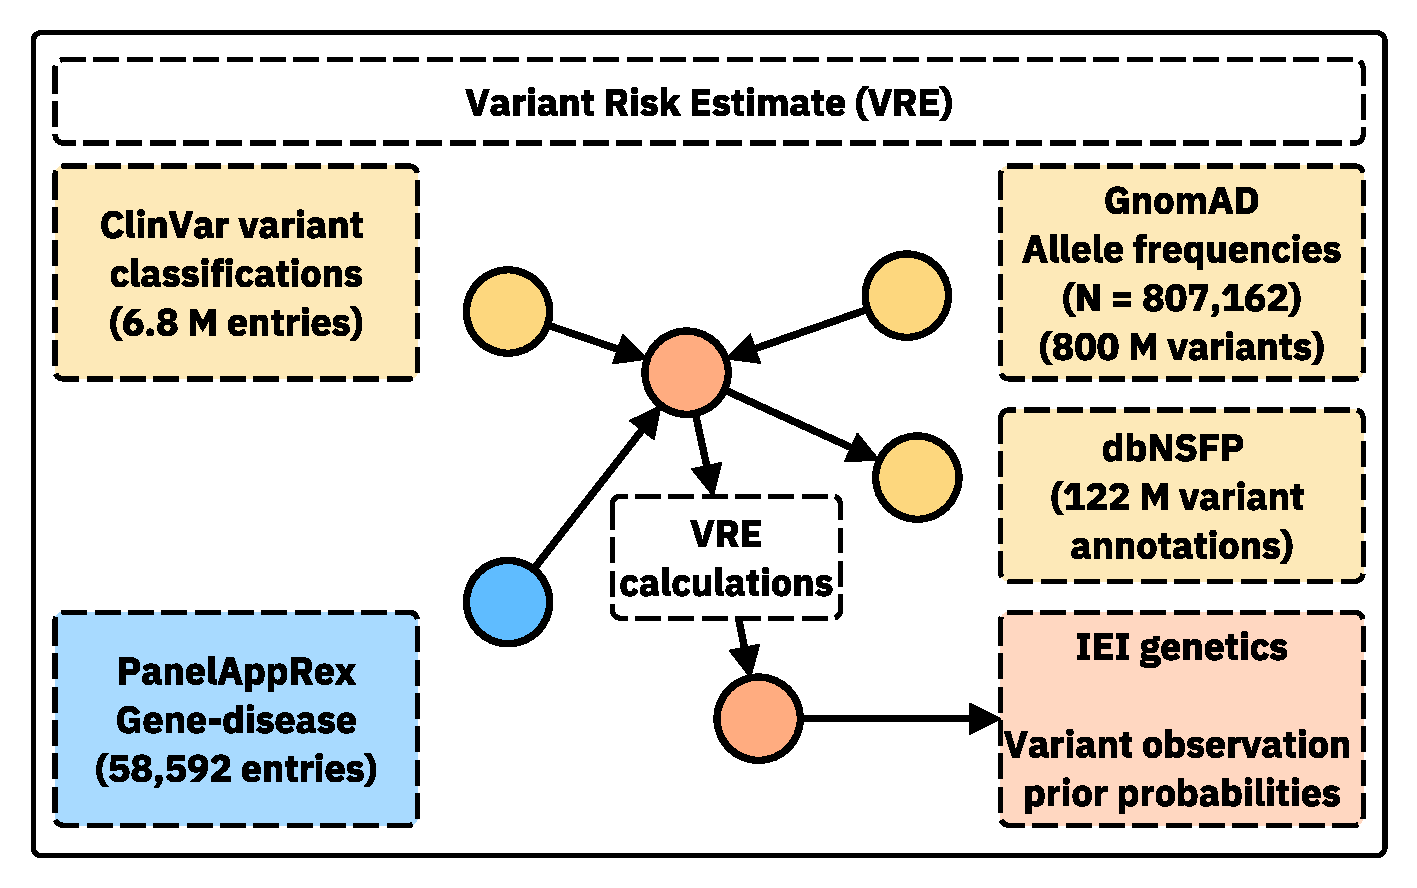
\includegraphics[width=0.99\textwidth]{../images/var_risk_est.pdf}

\clearpage

\section*{Acronyms}
\renewenvironment{description}%
  {\list{}{\labelwidth0pt\itemindent-\leftmargin
    \parsep-1em\itemsep0pt\let\makelabel\descriptionlabel}}
  {\endlist}
\begin{acronym}
 \acro{acmg}[ACMG]{American College of Medical Genetics and Genomics}
 \acro{acat}[ACAT]{Aggregated Cauchy Association Test}
 \acro{ad}[AD]{Autosomal Dominant}
 \acro{aid}[AID]{Autoinflammatory Disorders}
 \acro{anova}[ANOVA]{Analysis of Variance}
 \acro{ar}[AR]{Autosomal Recessive}
 \acro{bmf}[BMF]{Bone Marrow Failure}
 \acro{cd}[CD]{Complement Deficiencies}
 \acro{ci}[CI]{Confidence Interval}
 \acro{cid}[CID]{Immunodeficiencies affecting Cellular and Humoral Immunity}
 \acro{cid+}[CID+]{Combined Immunodeficiencies with Associated or Syndromic Features}
 \acro{cf}[CF]{Cystic Fibrosis}
 \acro{cftr}[\textit{CFTR}]{Cystic Fibrosis Transmembrane Conductance Regulator}
 \acro{cvid}[CVID]{Common Variable Immunodeficiency}
 \acro{dbnsfp}[dbNSFP]{database for Non-Synonymous Functional Predictions}
 \acro{ge}[GE]{Genomics England} 
 \acro{gnomad}[gnomAD]{Genome Aggregation Database}
 \acro{grch38}[GRCh38]{Genome Reference Consortium Human Build 38}
 \acro{hgvs}[HGVS]{Human Genome Variation Society}
 \acro{hpc}[HPC]{High-Performance Computing}
 \acro{hwe}[HWE]{Hardy-Weinberg Equilibrium}
 \acro{iei}[IEI]{Inborn Errors of Immunity}
  \acro{ig}[Ig]{Immunoglobulin}
 \acro{indel}[InDel]{Insertion/Deletion}
 \acro{iuis}[IUIS]{International Union of Immunological Societies}
 \acro{ld}[LD]{Linkage Disequilibrium}
 \acro{loeuf}[LOEUF]{Loss-Of-function Observed/Expected Upper bound Fraction}
  \acro{lof}[LOF]{Loss-of-Function}
 \acro{moi}[MOI]{Mode of Inheritance}
 \acro{nfkb1}[\textit{NFKB1}]{Nuclear Factor Kappa B Subunit 1}
 \acro{omim}[OMIM]{Online Mendelian Inheritance in Man}
 \acro{pad}[PAD]{Predominantly Antibody Deficiencies}
 \acro{pid}[PID]{Primary Immunodeficiency}
 \acro{pird}[PIRD]{Diseases of Immune Dysregulation}
 \acro{ppi}[PPI]{Protein-Protein Interaction}
 \acro{pli}[pLI]{Probability of being Loss-of-function Intolerant}
 \acro{snv}[SNV]{Single Nucleotide Variant}
 \acro{skat}[SKAT]{Sequence Kernel Association Test}
 \acro{stringdb}[STRINGdb]{Search Tool for the Retrieval of Interacting Genes/Proteins}
 \acro{hsd}[HSD]{Honestly Significant Difference}
 \acro{umap}[UMAP]{Uniform Manifold Approximation and Projection}
 \acro{uniprot}[UniProt]{Universal Protein Resource}
 \acro{vep}[VEP]{Variant Effect Predictor}
 \acro{xl}[XL]{X-Linked}
\end{acronym}



\section{Introduction}

In this study, we focused on reporting the probability of disease observation through genome-wide assessments of gene-disease combinations. Our central hypothesis was that by using highly curated annotation data including population allele frequencies, disease phenotypes, \ac{moi} patterns, and variant classifications and by applying rigorous calculations based on \ac{hwe}, we could accurately estimate the expected probabilities of observing disease-associated variants.
Among other benefits, this knowledge can be used to derive genetic diagnosis confidence by incorporating these new priors.

In this report, we focused on known \ac{iei} genes, also referred to as the \ac{pid} or Monogenic Inflammatory Bowel Disease genes \cite{tangye_human_2022, lawless_panelapprex_2025, martin_panelapp_2019} 
to validate our approach and demonstrate its clinical relevance. This application to a well-established genotype-phenotype set, comprising over 500 gene-disease associations, underscores its utility \cite{tangye_human_2022}.

Quantifying the risk that a newborn inherits a disease-causing variant is a fundamental challenge in genomics. Classical statistical approaches grounded in \ac{hwe} \cite{MayoCentury2008, AbramovsHardyWeinberg2020} have long been used to calculate genetic \ac{moi} probabilities for \ac{snv}s. However, applying these methods becomes more complex when accounting for different \ac{moi}, such as \ac{ar} versus \ac{ad} or \ac{xl} disorders. In AR conditions, for example, the occurrence probability must incorporate both the homozygous state and compound heterozygosity, whereas for \ac{ad} and \ac{xl} disorders, a single pathogenic allele is sufficient to cause disease. 
Advances in genetic research have revealed that \ac{moi} can be even more complex \cite{zschocke_mendelian_2023}. Mechanisms such as dominant negative effects, haploinsufficiency, mosaicism, and digenic or epistatic interactions can further modulate disease risk and clinical presentation, underscoring the need for nuanced approaches in risk estimation.
\citet{karczewski2020mutational} made significant advances; however, the remaining challenge lay in applying the necessary statistical genomics data across all MOI for any gene-disease combination 
Similar approaches have been reported for disease such Wilson disease, Mucopolysaccharidoses,  Primary ciliary dyskinesia, and treatable metabolic diseasse, 
\cite{bick_estimating_2025, evans_estimating_2021}, 
as reviewed by \citet{hannah_using_2024}.

To our knowledge all approaches to date have been limited to single \ac{moi}, specific to the given disease, or restricted to a small number of genes.
We argue that our integrated approach is highly powerful because the resulting probabilities can serve as informative priors in a Bayesian framework for variant and disease probability estimation; a perspective that is often overlooked in clinical and statistical genetics. Such a framework not only refines classical \ac{hwe}-based risk estimates but also has the potential to enrich clinicians’ understanding of what to expect in a patient and to enhance the analytical models employed by bioinformaticians.
The dataset also holds value for AI and reinforcement learning applications, providing an enriched version of the data underpinning frameworks such as AlphaFold \cite{jumper_highly_2021} and AlphaMissense \cite{cheng_accurate_2023}.

We introduced PanelAppRex to aggregate gene panel data from multiple sources, including \ac{ge} PanelApp, ClinVar, and \ac{uniprot}, thereby enabling advanced natural searches for clinical and research applications \cite{lawless_panelapprex_2025, martin_panelapp_2019, landrum_clinvar_2018, the_uniprot_consortium_uniprot_2025}. It automatically retrieves expert-curated panels, such as those from the NHS National Genomic Test Directory and the 100,000 Genomes Project, and converts them into machine-readable formats for rapid variant discovery and interpretation. We used PanelAppRex to label disease-associated variants.
We also integrate key statistical genomic resources. The gnomAD v4 dataset compiles data from 807,162 individuals, encompassing over 786 million \ac{snv}s and 122 million \ac{indel}s with detailed population-specific allele frequencies \cite{karczewski2020mutational}. \ac{dbnsfp} provides functional predictions for over 120 million potential non-synonymous and splicing-site SNVs, aggregating scores from 33 sources alongside allele frequencies from major populations \cite{liu_dbnsfp_2020}. ClinVar offers curated variant classifications such as ``Pathogenic'', ''Likely pathogenic'' and ``Benign'' mapped to HGVS standards and incorporating expert reviews \cite{landrum_clinvar_2018}.

%To cite: \url{https://doi.org/10.1016/j.gimo.2024.101881} \url{https://doi.org/10.1016/j.gim.2024.101284} and some from Eric's \url{https://www.cureffi.org/2019/06/05/using-genetic-data-to-estimate-disease-prevalence/}.

\section{Methods}
\subsection{Dataset}

Data from \ac{gnomad} v4 comprised 807,162 individuals, including 730,947 exomes and 76,215 genomes \cite{karczewski2020mutational}. This dataset provided 786,500,648 \ac{snv}s and 122,583,462 \ac{indel}s, with variant type counts of 9,643,254 synonymous, 16,412,219 missense, 726,924 nonsense, 1,186,588 frameshift and 542,514 canonical splice site variants. ClinVar data were obtained from the variant summary dataset (as of: 16 March 2025) available from the NCBI FTP site, and included 6,845,091 entries, which were processed into 91,319 gene classification groups and a total of 38,983 gene classifications; for example, the gene \textit{A1BG} contained four variants classified as likely benign and 102 total entries \cite{landrum_clinvar_2018}. For our analysis phase we also used \ac{dbnsfp} which consisted of a number of annotations for 121,832,908 \ac{snv}s 
\cite{liu_dbnsfp_2020}. 
The PanelAppRex core model contained 58,592 entries consisting of 52 sets of annotations, including the gene name, disease-gene panel ID, diseases-related features, confidence measurements.
\cite{lawless_panelapprex_2025}
A \ac{ppi} network data was provided by \ac{stringdb}, consisting of 19,566 proteins and 505,968 interactions \cite{szklarczyk2025string}.
The \ac{hgvs} nomenclature is used with \ac{vep}-based codes for variant IDs.
We carried out validations for disease cohorts with \ac{nfkb1} 
\cite{tuijnenburgNFKB12018,
who1997primary,
cunningham1999common,
oksenhendler2008infections}
and \ac{cftr} 
\cite{naito2023uk, castellani2013cftr2, Grasemann2023cftr}
to demonstrate applications in \ac{ad} and \ac{ar} disease genes, respectively.
AlphaMissense includes pathogenicity prediction classifications for 71 million variants in 19 thousand human genes \cite{cheng_accurate_2023, jun_cheng_2023_8208688}. We used these scores to compared against the probability of observing the same given variants.
\textbf{Box \ref{box:definitions}} list the definitions from the \ac{iuis} \ac{iei} for the major disease categories used throughout this study \cite{tangye_human_2022}.

\begin{tcolorbox}[colback=black!01, colframe=black!70, title=Box \ref{box:definitions} Definitions for IEI Major Disease Categories, label=box:definitions]
\textbf{Major Category} \hspace{4em} \textbf{Description}\\[5pt]
1. CID  Immunodeficiencies affecting cellular and humoral immunity\\[2pt]
2. CID+  Combined immunodeficiencies with associated or syndromic features\\[2pt]
3. PAD - Predominantly Antibody Deficiencies\\[2pt]
4. PIRD - Diseases of Immune Dysregulation\\[2pt]
5. PD - Congenital defects of phagocyte number or function\\[2pt]
6. IID - Defects in intrinsic and innate immunity\\[2pt]
7. AID - Autoinflammatory Disorders\\[2pt]
8. CD - Complement Deficiencies\\[2pt]
9. BMF - Bone marrow failure
\end{tcolorbox}

\subsection{Variant Class Observation Probability}
As a starting point, we considered the classical \ac{hwe} for a biallelic locus:
\[
p^2 + 2pq + q^2 = 1,
\]
where \(p\) is the allele frequency, \(q = 1 - p\), \(p^2\) represents the homozygous dominant, \(2pq\) the heterozygous, and \(q^2\) the homozygous recessive genotype frequencies. For disease phenotypes, particularly under \ac{ar} \ac{moi}, the risk is traditionally linked to the homozygous state (\(p^2\)); however, to account for compound heterozygosity across multiple variants, %we extend this by incorporating the contribution from other pathogenic alleles.
we allocated the overall gene‐level risk proportionally among variants.

Our computational pipeline estimated the probability of observing a disease-associated genotype for each variant and aggregated these probabilities by gene and ClinVar classification. This approach included all variant classifications, not limited solely to those deemed ``pathogenic'', and explicitly conditioned the classification on the given phenotype, recognising that a variant could only be considered pathogenic relative to a defined clinical context. The core calculations proceeded as follows:

\paragraph{1. Allele Frequency and Total Variant Frequency.} 
\label{sec:min_risk}
For each variant \(i\) in a gene, the allele frequency was denoted as \(p_i\). For each gene, we defined the total variant frequency (summing across all reported variants in that gene) as:

\[P_{\text{tot}} = \sum_{i \in \text{gene}} p_i.\]

If any of the possible \ac{snv}  had no observed allele (\(p_i = 0\)), we assigned a minimal risk:

\[p_i = \frac{1}{\max(AN) + 1}\]

where \(\max(AN)\) was the maximum allele number observed for that gene. This adjustment ensured that a nonzero risk was incorporated even in the absence of observed variants.

\paragraph{2. Occurrence Probability Based on \ac{moi}.}
The probability that an individual was affected by a variant depended on the \ac{moi} relative to a specific phenotype. Specifically, we calculated the occurrence probability \(p_{\text{disease},i}\) for each variant as follows:
\begin{itemize}
    \item For \textbf{\ac{ad}} and \textbf{\ac{xl}} variants, a single copy was sufficient, so
    \[
    p_{\text{disease},i} = p_i.
    \]
    \item For \textbf{\ac{ar}} variants, disease is expected to manifest when two pathogenic alleles were present. In this case, we accounted for both the homozygous state and the possibility of compound heterozygosity.
     We allocated the overall gene‐level risk ($P_{\text{tot}}^2$) proportionally by variant allele frequency:
% version 1 is wrong because it counted het variants twice: \[ p_{\text{disease},i} = p_i^2 + 2\,p_i\bigl(P_{\text{tot}} - p_i\bigr). \]
    \[p_{\text{disease},i} = p_i \; P_{\text{tot}}.\] % version 2
\end{itemize}

\paragraph{3. Expected Case Numbers and Case Detection Probability.}
Given a population with \(N\) births (e.g. as seen in our validation studies, \(N = 69\,433\,632\)), the expected number of cases attributable to variant \(i\) was calculated as:

\[
E_i = N \cdot p_{\text{disease},i}.
\]

The probability of detecting at least one affected individual for that variant was computed as:

\[
P(\geq 1)_i = 1 - \bigl(1 - p_{\text{disease},i}\bigr)^N.
\]

\paragraph{4. Aggregation by Gene and ClinVar Classification.}
For each gene and for each ClinVar classification (e.g. ``Pathogenic'', ``Likely pathogenic'', ``Uncertain significance'', etc.), we aggregated the results across all variants. The total expected cases for a given group was:

\[
E_{\text{group}} = \sum_{i \in \text{group}} E_i,
\]

and the overall probability of observing at least one case within the group was calculated as:

\[
P_{\text{group}} = 1 - \prod_{i \in \text{group}} \left(1 - p_{\text{disease},i}\right).
\]

\paragraph{5. Data Processing and Implementation.}
We implemented the calculations within a \ac{hpc} pipeline and provided an example for a single dominant disease gene, \textit{TNFAIP3}, in the source code to enhance reproducibility. Variant data were imported in chunks from the annotation database for all chromosomes (1-22, X, Y, M). 

For each data chunk, the relevant fields were gene name, position, allele number, allele frequency, ClinVar classification, and HGVS annotations. Missing classifications (denoted by ``.'') were replaced with zeros and allele frequencies were converted to numeric values. We then retained only the first transcript allele annotation for simplicity, as the analysis was based on genomic coordinates. Subsequently, the variant data were merged with gene panel data from PanelAppRex to obtain the disease-related \ac{moi} mode for each gene. For each gene, if no variant was observed for a given ClinVar classification (i.e. \(p_i = 0\)), a minimal risk was assigned as described above. Finally, we computed the occurrence probability, expected cases, and the probability of observing at least one case using the equations presented.

The final results were aggregated by gene and ClinVar classification and used to generate summary statistics that reviewed the predicted disease observation probabilities.


\subsection{Validation of Autosomal Dominant Estimates Using \textit{NFKB1}}

To validate our genome-wide probability estimates in an \ac{ad} gene, we focused on \ac{nfkb1}. Our goal was to compare the expected number of \ac{nfkb1}-related \ac{cvid} cases, as predicted by our framework, with the reported case count in a well-characterised national-scale \ac{pid} cohort.

\paragraph{1. Reference Dataset.}
We used a reference dataset reported by \citet{tuijnenburgNFKB12018} to build a validation model in an \ac{ad} disease gene. This study performed whole‐genome sequencing of 846 predominantly sporadic, unrelated \ac{pid} cases from the NIHR BioResource-Rare Diseases cohort. There were 390 \ac{cvid} cases in the cohort. The study identified \ac{nfkb1} as one of the genes most strongly associated with \ac{pid}. Sixteen novel heterozygous variants including truncating, missense, and gene deletion variants, were found in \ac{nfkb1} among the \ac{cvid} cases.

\paragraph{2. Cohort Prevalence Calculation.}
Within the cohort, 16 out of 390 \ac{cvid} cases were attributable to \ac{nfkb1}. Thus, the observed cohort prevalence was
\[
\text{Prevalence}_{\text{cohort}} = \frac{16}{390} \approx 0.041,
\]
with a 95\% confidence interval (using Wilson's method) of approximately \((0.0254,\,0.0656)\).

\paragraph{3. National Estimate Based on Literature.}
Based on literature, the prevalence of \ac{cvid} in the general population was estimated as
\[
\text{Prevalence}_{\text{CVID}} = \frac{1}{25\,000}.
\]
For a UK population of 
\[
N_{\text{UK}} \approx 69\,433\,632,
\]
the expected total number of \ac{cvid} cases was
\[
E_{\text{CVID}} \approx \frac{69\,433\,632}{25\,000} \approx 2777.
\]
Assuming that the proportion of \ac{cvid} cases attributable to \ac{nfkb1} is equivalent to the cohort estimate, the literature extrapolated estimate is
\[
\text{Estimated NFKB1 cases} \approx 2777 \times 0.041 \approx 114,
\]
with a median value of approximately 118 and a 95\% confidence interval of 70 to 181 cases (derived from posterior sampling).

\paragraph{4. Bayesian Adjustment.}
Recognising that the clinical cohort likely represents nearly all \ac{cvid} cases (besides first-second degree relatives), two Bayesian adjustments were performed:
\begin{enumerate}
  \item \textbf{Weighted Adjustment (emphasising the cohort, \(w=0.9\)):}
  \[
  \text{Adjusted Estimate} = 0.9 \times 16 + 0.1 \times 114 \approx 26,
  \]
  with a corresponding 95\% confidence interval of approximately 21 to 33 cases.
  
  \item \textbf{Mixture Adjustment (equal weighting, \(w=0.5\)):}  
  Posterior sampling of the cohort prevalence was performed assuming
  \[
  p \sim \mathrm{Beta}(16+1,\,390-16+1),
  \]
  which yielded a Bayesian mixture adjusted median estimate of 67 cases with a 95\% credible interval of approximately 43 to 99 cases.
\end{enumerate}

\paragraph{5. Predicted Total Genotype Counts.}
The predicted total synthetic genotype count (before adjustment) was 456, whereas the predicted total genotypes adjusted for \texttt{synth\_flag} was 0. This higher synthetic count was set based on a minimal risk threshold, ensuring that at least one genotype is assumed to exist (e.g. accounting for a potential unknown de novo variant) even when no variant is observed in gnomAD (as per \textbf{section
\ref{sec:min_risk}}).

\paragraph{6. Validation Test.}
Thus, the expected number of \ac{nfkb1}-related \ac{cvid} cases derived from our genome-wide probability estimates was compared with the observed counts from the UK-based \ac{pid} cohort. This comparison validates our framework for estimating disease incidence in \ac{ad} disorders.

% Annotated key values from R:
% Predicted total genotypes (adjusted for synth_flag): 0 
% Predicted total synthetic genotype count: 456 
% Reported NFKB1-related CVID cases (n_NFKB1): 16 
% Literature extrapolated estimate median: 118 
% 95% CI for literature extrapolated estimate: [70, 181] 
% Bayesian mixture adjusted estimate (w = 0.5) median: 67 
% 95% CI for Bayesian mixture adjusted estimate: [43, 99] 
% Bayesian adjusted estimated number of NFKB1-related CVID cases (w = 0.9): 26 
% 95% Bayesian adjusted CI (w = 0.9): [21, 33]

\subsection{Validation Study for Autosomal Recessive CF Using CFTR}

To validate our framework for \ac{ar} diseases, we focused on \ac{cf}.
For comparability sizes between the validation studies, we analysed the most common \ac{snv} in the \ac{cftr} gene, typically reported as ``p.Arg117His'' (GRCh38 Chr 7:117530975 G/A, MANE Select HGVSp ENST00000003084.11: p.Arg117His).
Our goal was to validate our genome-wide probability estimates by comparing the expected number of \ac{cf} cases attributable to the p.Arg117His variant in \ac{cftr} with the nationally reported case count in a well-characterised disease cohort
\cite{naito2023uk, castellani2013cftr2, Grasemann2023cftr}.

\paragraph{1. Expected Genotype Counts.}
Let \( p \) denote the allele frequency of the p.Arg117His variant and \( q \) denote the combined frequency of all other pathogenic \ac{cftr} variants, such that
\[
q = P_{\text{tot}} - p \quad \text{with} \quad P_{\text{tot}} = \sum_{i \in \text{CFTR}} p_i.
\]
Under Hardy–Weinberg equilibrium for an \ac{ar} trait, the expected frequencies were:
\[
f_{\text{hom}} = p^2 \quad \text{(homozygous for p.Arg117His)}
\]
and
\[
f_{\text{comphet}} = 2p\,q \quad \text{(compound heterozygotes carrying p.Arg117His and another pathogenic allele)}.
\]
For a population of size \( N \) (here, \( N \approx 69\,433\,632 \)), the expected number of cases were:
\[
E_{\text{hom}} = N \cdot p^2,\quad E_{\text{comphet}} = N \cdot 2p\,q,\quad E_{\text{total}} = E_{\text{hom}} + E_{\text{comphet}}.
\]

\paragraph{2. Mortality Adjustment.}
Since \ac{cf} patients experience increased mortality, we adjusted the expected genotype counts using an exponential survival model \cite{naito2023uk, castellani2013cftr2, Grasemann2023cftr}. With an annual mortality rate \(\lambda \approx 0.004\) and a median age of 22 years, the survival factor was computed as:
\[
S = \exp(-\lambda \cdot 22).
\]
Thus, the mortality-adjusted expected genotype count became:
\[
E_{\text{adj}} = E_{\text{total}} \times S.
\]

\paragraph{3. Bayesian Uncertainty Simulation.}
To incorporate uncertainty in the allele frequency \( p \), we modelled \( p \) as a beta-distributed random variable:
\[
p \sim \mathrm{Beta}(p \cdot \text{AN}_{\text{eff}} + 1,\; \text{AN}_{\text{eff}} - p \cdot \text{AN}_{\text{eff}} + 1),
\]
using a large effective allele count (\(\text{AN}_{\text{eff}}\)) for illustration. By generating 10,000 posterior samples of \( p \), we obtained a distribution of the literature-based adjusted expected counts, \(E_{\text{adj}}\).

\paragraph{4. Bayesian Mixture Adjustment.}
Since the national registry may not capture all nuances (e.g., reduced penetrance) of \ac{cftr}-related disease, we further combined the literature-based estimate with the observed national count (714 cases from the UK Cystic Fibrosis Registry 2023 Annual Data Report) using a 50:50 weighting:
\[
E_{\text{Bayes}} = 0.5 \times (\text{Observed Count}) + 0.5 \times E_{\text{adj}}.
\]

\paragraph{5. Validation test.}
Thus, the expected number of \ac{cftr}-related \ac{cf} cases derived from our genome-wide probability estimates was compared with the observed counts from the UK-based \ac{cf} registry. This comparison validated our framework for estimating disease incidence in \ac{ad} disorders.


\subsection{Validation of SCID-specific Estimates Using PID–SCID Genes}

To validate our genome-wide probability estimates for diagnosing a genetic variant in a patient with a PID phenotype, we focused on a subset of genes implicated in Severe Combined Immunodeficiency (SCID). Given that the overall panel corresponds to PID, but SCID represents a rarer subset, the probabilities were converted to values per million PID cases.

\paragraph{1. Incidence Conversion.}
Based on literature, PID occurs in approximately 1 in 1,000 births, whereas SCID occurs in approximately 1 in 100,000 births. Consequently, in a population of 1,000,000 births there are about 1,000 PID cases and 10 SCID cases. To express SCID-related variant counts on a per-million PID scale, the observed SCID counts were multiplied by 100. For example, if a gene is expected to cause SCID in 10 cases within the total PID population, then on a per-million PID basis the count is 10 × 100 = 1,000 cases (across all relevant genes).

\paragraph{2. Prevalence Calculation and Data Adjustment.}
For each SCID-associated gene (e.g. \textit{IL2RG}, \textit{RAG1}, \textit{DCLRE1C}), the observed variant counts in the dataset were adjusted by multiplying by 100 so that the probabilities reflect the expected number of cases per 1,000,000 PID. In this manner, our estimates are directly comparable to known counts from SCID cohorts, rather than to national population counts as in previous validation studies.

\paragraph{3. Integration with Prior Probability Estimates.}
The predicted genotype occurrence probabilities were derived from our framework across the PID gene panel. These probabilities were then converted to expected case counts per million PID cases by multiplying by 1,000,000. For instance, if the probability of observing a pathogenic variant in \textit{IL2RG} is \(p\), the expected SCID-related count becomes \(p \times 10^6\). Similar conversions are applied for all relevant SCID genes.

\paragraph{4. Bayesian Uncertainty and Comparison with Observed Data.}
To address uncertainty in the SCID-specific estimates, a Bayesian uncertainty simulation was performed for each gene to generate a distribution of predicted case counts on a per-million PID scale. The resulting median estimates and 95\% credible intervals were then compared against known national SCID counts compiled from independent registries. This comparison permited a direct evaluation of our framework’s accuracy in predicting the occurrence of SCID-associated variants within a PID cohort.

\paragraph{5. Validation Test.}
Thus, by converting the overall probability estimates to a per-million PID scale, our framework was directly validated against observed counts for SCID. %This procedure confirms that our probability estimation approach can be effectively adapted to specific subphenotypes within a broader disease spectrum, ensuring robust application for both global PID and SCID diagnostics.


\subsection{Protein Network and Genetic Constraint Interpretation}
A \ac{ppi} network was constructed using protein interaction data from \ac{stringdb} \cite{szklarczyk2025string}. We previously prepared and reported 
on this dataset consisting of 19,566 proteins and 505,968 interactions 
(\url{https://github.com/DylanLawless/ProteoMCLustR}).
Node attributes were derived from log-transformed score-positive-total values, which informed both node size and colour. Top-scoring nodes (top 15 based on score) were labelled to highlight prominent interactions. To evaluate group differences in score-positive-total across major disease categories, one-way \ac{anova} was performed followed by Tukey \ac{hsd} post hoc tests (and non-parametric Dunn’s test for confirmation). 
GnomAD v4.1 constraint metrics data was used for the \ac{ppi} analysis and was sourced from \citet{karczewski2020mutational}.
This provided transcript-level metrics, such as observed/expected ratios, \ac{loeuf}, pLI, and Z-scores, quantifying loss-of-function and missense intolerance, along with confidence intervals and related annotations for 211,523 observations.

\subsection{Gene Set Enrichment Test}

To test for overrepresentation of biological functions, the prioritised genes were compared against gene sets from MsigDB (including hallmark, positional, curated, motif, computational, GO, oncogenic, and immunologic signatures) and WikiPathways using hypergeometric tests with FUMA \cite{watanabe_functional_2017, liberzon_molecular_2011}. The background set consisted of 24,304 genes. Multiple testing correction was applied per data source using the Benjamini-Hochberg method, and gene sets with an adjusted P-value $\le$ 0.05 and more than one overlapping gene are reported.

\subsection{Deriving novel PID classifications by genetic PPI and clinical features}
We recategorised 315 immunophenotypic features from the original \ac{iuis} \ac{iei} annotations, reducing the original multi‐level descriptors (e.g. ``decreased cd8, normal or decreased cd4'') first to 
minimal labels (e.g.``low'') and second to binary outcomes (normal vs. not-normal) for T cells, B cells, neutrophils, and immunoglobulins %(\textbf{Figure \ref{fig:immunophenotype_before_after}}). 
Each gene was mapped to its \ac{ppi} cluster derived from STRINGdb and UMAP embeddings from previous steps. 
We first tested for non‐random associations between these four binary immunophenotypes and PPI clusters using $\chi^2$ tests. %(see Figure \ref{fig:multicat_patch_3_clust_chi}). 
To generate a data‐driven PID classification, we trained a decision tree (rpart) to predict PPI cluster membership from the four immunophenotypic features plus the traditional IUIS Major and Subcategory labels. Hyperparameters (complexity parameter = 0.001, minimum split = 10, minimum bucket = 5, maximum depth = 30) were optimised via five‐fold cross validation using the \texttt{caret} framework. Terminal node assignments were then relabelled according to each group’s predominant abnormal feature profile.

\subsection{Probability of observing AlphaMissense pathogenicity}
We obtained the subset pathogenicity predictions from AlphaMissense via the AlphaFold database and whole genome data from the studies data repository\cite{cheng_accurate_2023, jun_cheng_2023_8208688}. 
The AlphaMissense data (genome‐aligned and amino acid substitutions) were merged with the panel variants based on genomic coordinate and HGVSc annotation. 
Occurrence probabilities were log-transformed and adjusted (y-axis displaying log10(occurrence prob + 1e-5) + 5)), to visualise the distribution of pathogenicity scores across the residue sequence. 
A Kruskal-Wallis test was used to compare the observed disease probability across clinical classification groups.

\section{Results}

\subsection{Observation Probability Across Disease Genes}

Our study integrated large-scale annotation databases with gene panels from PanelAppRex to systematically assess disease genes by MOI. By combining population allele frequencies with ClinVar clinical classifications, we computed an expected observation probability for each SNV, representing the likelihood of encountering a variant of a specific pathogenicity for a given phenotype. We report these probabilities for 54,814 ClinVar variant classifications across 557 genes (linked dataset \cite{lawless_2025_15111584}).

In practice, our approach computed a simple observation probability for every SNV across the genome and was applicable to any disease-gene panel. Here, we focused on panels related to Primary Immunodeficiency or Monogenic Inflammatory Bowel Disease, using PanelAppRex panel ID 398 as a case study.
\textbf{Figure \ref{fig:p_varRisEst_summary_scores}} displays all reported ClinVar  variant classifications for this panel. The resulting natural scaling system (-5 to +5) accounts for the frequently encountered combinations of classification labels (e.g. benign to pathogenic).
The resulting data set \cite{lawless_2025_15111584} is briefly shown in \textbf{Table \ref{tab:head_result_table}} to illustrate that our method yielded estimations of the probability of observing a variant with a particular ClinVar classification. 

%This framework, of pre-calculated disease-related variant occurrence probabilities, enabled comprehensive analyses across the entire genome, paving the way for rapid assessment of variant significance in diverse disease contexts.

\begin{table}[ht]
\centering
\caption{Example of the first several rows from our main results for 557 genes of PanelAppRex's panel: (ID 398) Primary immunodeficiency or monogenic inflammatory bowel disease. ``ClinVar Significance'' indicates the pathogenicity classification assigned by ClinVar, while inVar Significance'' indicates the pathogenicity classification assigned by ClinVar, while ``Occurrence Prob'' represents our calculated probability of observing the corresponding variant class for a given phenotype. Additional columns, such as population allele frequency, are not shown. \cite{lawless_2025_15111584}}
\label{tab:head_result_table} 
\centering
\resizebox{\ifdim\width>\linewidth\linewidth\else\width\fi}{!}{
\begin{tabular}[t]{lrlrllll}
\toprule
Gene & Panel ID & ClinVar Clinical Significance & GRCh38 Pos & HGVSc (VEP) & HGVSp (VEP) & Inheritance & Occurrence Probability\\
\midrule
ABI3 & 398 & Uncertain significance & 49210771 & c.47G>A & p.Arg16Gln & AR & 0.000000007\\
ABI3 & 398 & Uncertain significance & 49216678 & c.265C>T & p.Arg89Cys & AR & 0.000000005\\
ABI3 & 398 & Uncertain significance & 49217742 & c.289G>A & p.Val97Met & AR & 0.000000002\\
ABI3 & 398 & Uncertain significance & 49217781 & c.328G>A & p.Gly110Ser & AR & 0.000000002\\
ABI3 & 398 & Uncertain significance & 49217844 & c.391C>T & p.Pro131Ser & AR & 0.000000015\\
\addlinespace
ABI3 & 398 & Uncertain significance & 49220257 & c.733C>G & p.Pro245Ala & AR & 0.000000022\\
\bottomrule
\end{tabular}}
\end{table}


\begin{figure}[ht]
  \centering
  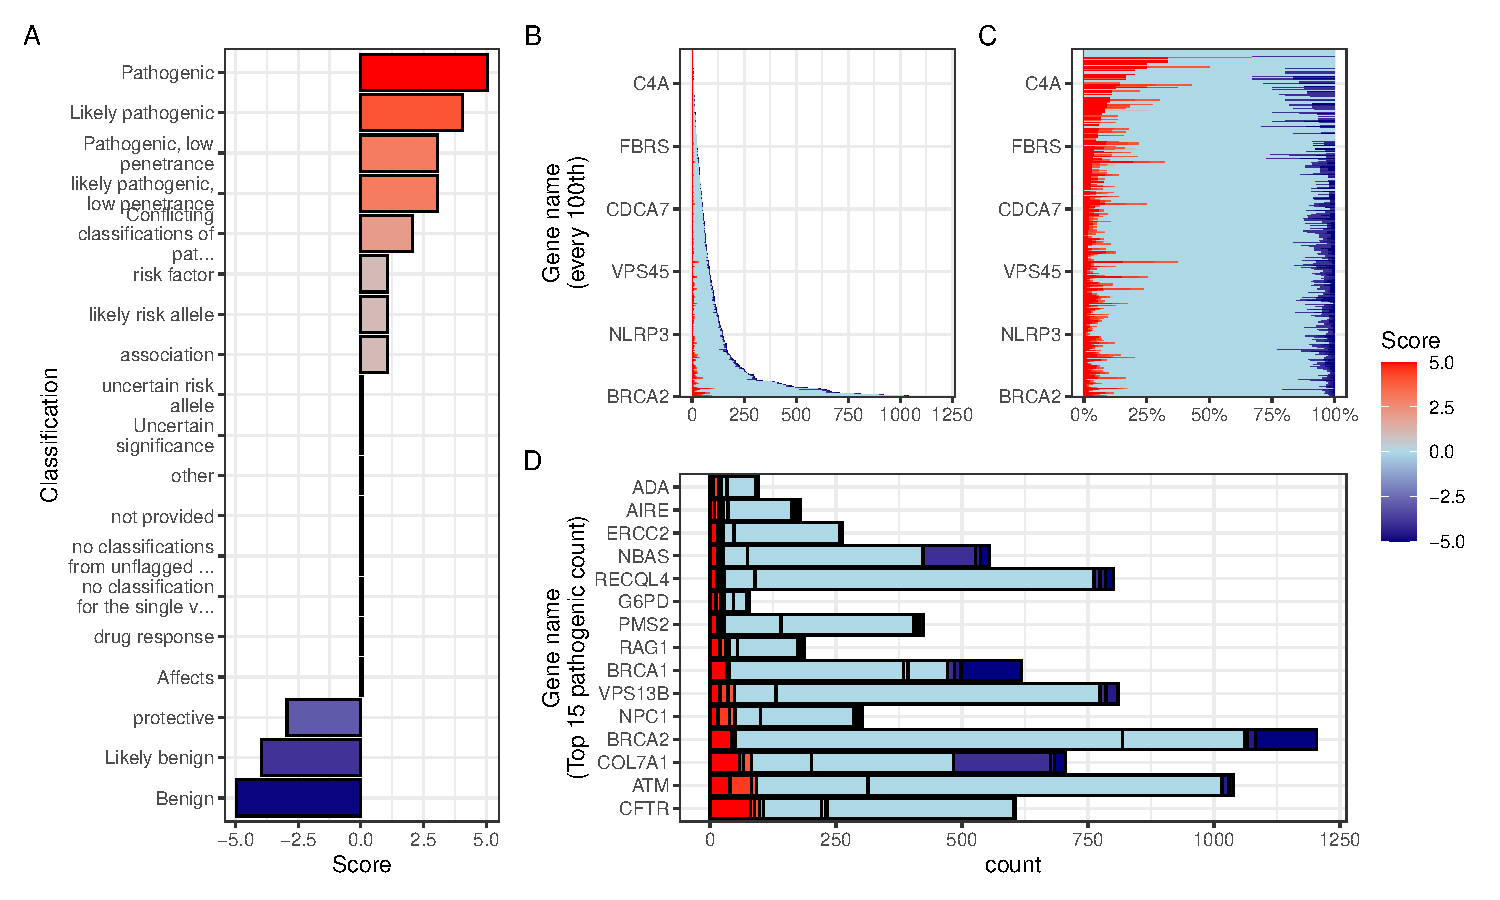
\includegraphics[width=0.99\textwidth]{../images/p_varRisEst_summary_scores.pdf}
  \caption{\textbf{Summary of ClinVar clinical significance classifications in the \ac{pid} gene panel.} (A) Shows the numeric score coding for each classification. Panels (B) and (C) display the tally of classifications per gene as absolute counts and as percentages, respectively. (D) Highlights the top 15 genes with the highest number of reported pathogenic classifications (score 5).}
  \label{fig:p_varRisEst_summary_scores}
\end{figure}

%\subsection{Validation studies}
%\subsubsection{Validation of Dominant Disease Occurrence with \textit{NFKB1}}
%
%THESE VALUES ARE WRONG BECAUSE I USE THE n-cvid INSTEAD OF n-nfkb1 VARIABLE. FIX VALUES TO MATCH THE CORRECTED PLOT. we have 3 total synth de novo and 2 count as P score for the locus zoom plot: (P, P/LP, LP).
%
%To validate our genome-wide probability estimates for \ac{ad} disorders, we focused on \ac{nfkb1}. We used a reference dataset from \citet{tuijnenburgNFKB12018}, in which whole‐genome sequencing of 846 \ac{pid} patients identified \ac{nfkb1} as one of the genes most strongly associated with the disease, with 390 \ac{cvid} cases attributed to heterozygous variants. Our goal was to compare the predicted number of \ac{nfkb1}-related \ac{cvid} cases with the reported count in this well-characterised national-scale cohort.
%
%Our model calculated 456 \ac{nfkb1}-related \ac{cvid} cases in the UK. In the reference cohort,  390  \ac{nfkb1} \ac{cvid} cases were reported. 
%We additionally wanted to account for potential under-reporting in the reference study.
%We used an extrapolated national \ac{cvid} prevalence to yield an upper bound maximum of 1280 cases (95\% \ac{ci}: 1188–1374), while a Bayesian-adjusted mixture estimate produced a median of 835 cases (95\% \ac{ci}: 789–882). 
%\textbf{Figure \ref{fig:validation_studies_bayesian_adjusted_estimates} (A)}
%illustrates that our predicted value of 456 lies within these ranges and is closer to the observed count, thereby supporting the validity of our integrated probability estimation framework for \ac{ad} disorders.

\subsection{Validation studies}
\subsubsection{Validation of Dominant Disease Occurrence with \textit{NFKB1}}

To validate our genome-wide probability estimates for \ac{ad} disorders, we focused on \ac{nfkb1}. We used a reference dataset from \citet{tuijnenburgNFKB12018}, in which whole‐genome sequencing of 846 \ac{pid} patients identified \ac{nfkb1} as one of the genes most strongly associated with the disease, with 16 \ac{nfkb1}-related \ac{cvid} cases attributed to \ac{ad} heterozygous variants. Our goal was to compare the predicted number of \ac{nfkb1}-related \ac{cvid} cases with the reported count in this well-characterised national-scale cohort.

Our model calculated 0 known pathogenic variant \ac{nfkb1}-related \ac{cvid} cases in the UK with a minimal risk of 456 unknown de novo variants. In the reference cohort, 16 \ac{nfkb1} \ac{cvid} cases were reported. We additionally wanted to account for potential under-reporting in the reference study. We used an extrapolated national \ac{cvid} prevalence which yielded a median estimate of 118 cases (95\% CI: 70–181), while a Bayesian-adjusted mixture estimate produced a median of 67 cases (95\% CI: 43–99). \textbf{Figure \ref{fig:validation_studies_bayesian_adjusted_estimates} (A)} illustrates that our predicted values reflect these ranges and are closer to the observed count. This case supports the validity of our integrated probability estimation framework for \ac{ad} disorders, and represents a challenging example where pathogenic \ac{snv} are not reported in the reference population of gnomAD. Our min-max values successfully contained the true reported values.


\subsubsection{Validation of Recessive Disease Occurrence with \textit{CFTR}}

Our analysis predicted the number of \ac{cf} cases attributable to carriage of the p.Arg117His variant (either as homozygous or as compound heterozygous with another pathogenic allele) in the UK. Based on \ac{hwe} calculations and mortality adjustments, we predicted approximately 648 cases arising from biallelic variants and 160 cases from homozygous variants, resulting in a total of 808 expected cases.

In contrast, the nationally reported number of \ac{cf} cases was 714, as recorded in the UK Cystic Fibrosis Registry 2023 Annual Data Report
\cite{naito2023uk}. To account for factors such as reduced penetrance and the mortality-adjusted expected genotype, we derived a Bayesian-adjusted estimate via posterior simulation. Our Bayesian approach yielded a median estimate of 740 cases (95\% \ac{ci}: 696, 786) and a mixture-based estimate of 727 cases (95\% \ac{ci}: 705, 750).
\textbf{Figure \ref{fig:validation_studies_bayesian_adjusted_estimates} (B)} illustrates the close concordance between the predicted values, the Bayesian-adjusted estimates, and the national report supports the validity of our approach for estimating disease.


\textbf{Figure \ref{fig:validation_scatter_dense}} shows the final values for these genes of interest in a given population size and phenotype. It reveals that an allele frequency threshold of approximately 0.000007 is required to observe a single heterozygous disease-causing variant carrier in the UK population for both genes. However, owing to the \ac{ar} \ac{moi} pattern of \ac{cftr}, this threshold translates into more than 100,000 heterozygous carriers, compared to only 456 carriers for the \ac{ad} gene \ac{nfkb1}. Note that this allele frequency threshold, being derived from the current reference population, represents a lower bound that can become more precise as public datasets continue to grow. This marked difference underscores the significant impact of \ac{moi} patterns on population carrier frequencies and the observed disease prevalence.




\FloatBarrier
\subsubsection{Interpretation of ClinVar Variant Observations}

\textbf{Figure~\ref{fig:all_genes_combined_bar_charts_mini}} shows  the two validation study \ac{pid} genes, representing \ac{ar} and dominant \ac{moi}. \textbf{Figure~\ref{fig:all_genes_combined_bar_charts_mini} (A)}   illustrates the overall probability of an affected birth by ClinVar variant classification, whereas \textbf{Figure~\ref{fig:all_genes_combined_bar_charts_mini}  (B)}  depicts the total expected number of cases per classification for an example population, here the UK, of approximately 69.4 million. 

\subsubsection{Validation of SCID-specific Disease Occurrence}

Given that SCID is a subset of PID, our probability estimates reflect the likelihood of observing a genetic variant as a diagnosis when the phenotype is PID. However, we additionally tested our results against SCID cohorts in 
 \textbf{Figure \ref{fig:scid_combined}}.
 The summarised raw cohort data for SCID-specific gene counts are summarised and compared across countries in \textbf{Figure \ref{fig:scid_gene_comparison}}.
True counts for \textit{IL2RG} and \textit{DCLRE1C} from ten distinct locations yielded 95\% confidence intervals surrounding our predicted values. For \textit{IL2RG}, the prediction was low (approximately 1 case per 1,000,000 PID), as expected since loss-of-function variants in this X-linked gene are highly deleterious and rarely observed in gnomAD. In contrast, the predicted value for \textit{RAG1} was substantially higher (553 cases per 1,000,000 PID) than the observed counts (ranging from 0 to 200). We attributed this discrepancy to the lower penetrance and higher background frequency of \textit{RAG1} variants in recessive inheritance, whereby reference studies may underreport the true national incidence. Overall, we argued that agreement within an order of magnitude was tolerable given the inherent uncertainties from reference studies arising from variable penetrance and allele frequencies.

\FloatBarrier
\subsection{Genetic constraint in high-impact protein networks}

We next examined genetic constraint in high-impact protein networks across the whole \ac{iei} gene set of over 500 known disease-gene phenotypes \cite{tangye_human_2022}. By integrating ClinVar variant classification scores with \ac{ppi} data, we quantified the pathogenic burden per gene and assessed its relationship with network connectivity and genetic constraint
\cite{szklarczyk2025string, karczewski2020mutational}.

\subsubsection{Score-Positive-Total within IEI PPI network}

The ClinVar classifications reported in 
\textbf{Figure \ref{fig:p_varRisEst_summary_scores}} were scaled -5 to +5 based on their pathogenicity. 
We were interested in positive (potentially damaging) but not negative (benign) scoring variants, which are statistically incidental in this analysis. 
We tallied gene-level positive scores to give the score positive total metric. 
\textbf{Figure \ref{fig:ppi_network_assoc} (A)} shows the \ac{ppi} network of disease-associated genes, where node size and colour encode the score positive total (log-transformed). 
The top 15 genes with the highest total prior probabilities of being observed with disease are labelled (as per \textbf{Figure \ref{fig:p_varRisEst_summary_scores}}).

\begin{figure}[ht]
  \centering
  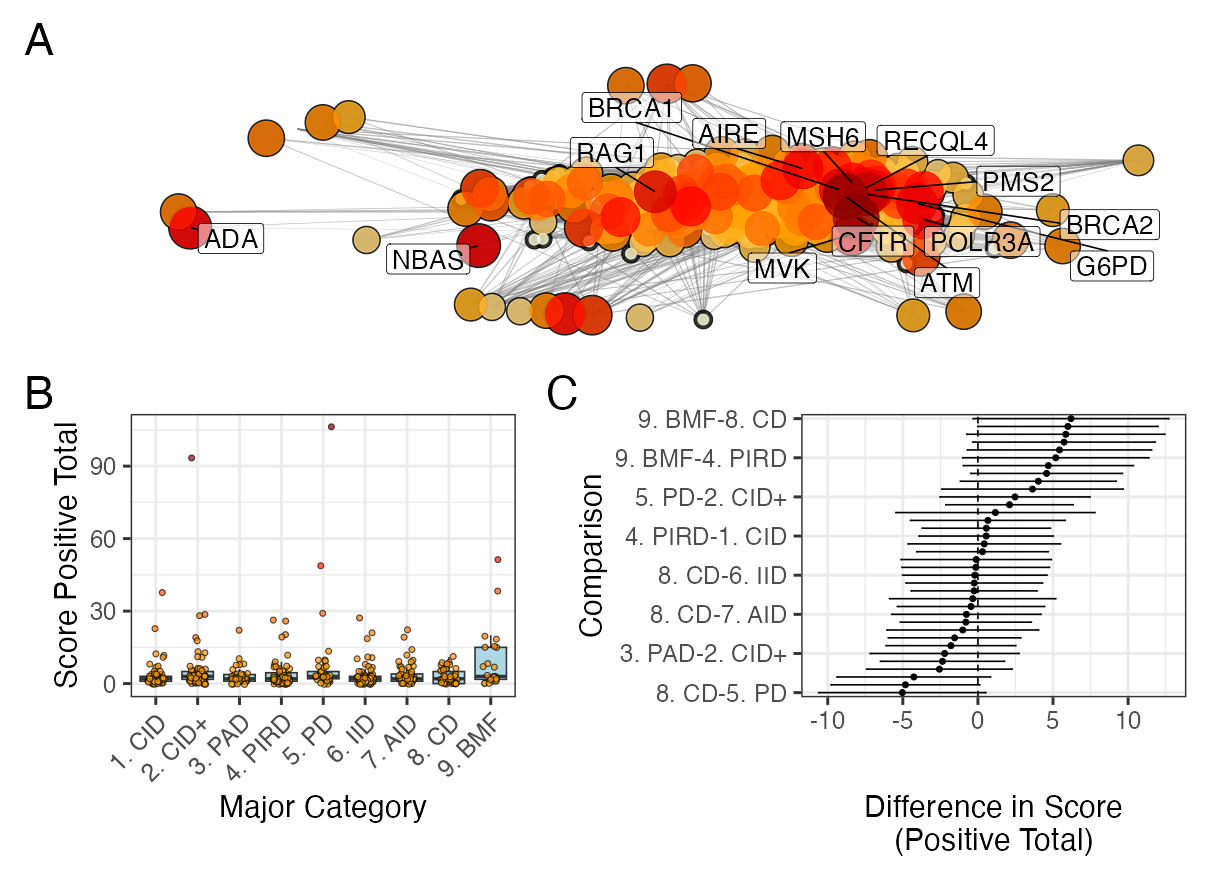
\includegraphics[width=\textwidth]{../images/untangleR_ppi_network_assoc_patch1.jpg}
  \caption{\textbf{\ac{ppi} network and score positive total ClinVar significance variants}.
    (A) \ac{ppi} network of disease-associated genes. Node size and colour represent the log-transformed score positive total, the top 15 genes/proteins with the highest probability of being observed in disease are labelled.
    (B) Distribution of score positive total across the major \ac{iei} disease categories.
    (C) Tukey \ac{hsd} comparisons of mean differences in score positive total among all pairwise disease categories. Every 5th label is shown on y-axis.
  }
  \label{fig:ppi_network_assoc}
\end{figure}





\FloatBarrier
\subsubsection{Association Analysis of Score-Positive-Total across IEI Categories} 

We checked for any statistical enrichment in score positive totals, which represents the expected observation of pathogenicity, between the \ac{iei} categories.
The one‐way \ac{anova} revealed an effect of major disease category on score positive total (\(F(8,500)=2.82,\,p=0.0046\)), indicating that group means were not identical, which we observed in
\textbf{Figure \ref{fig:ppi_network_assoc} (B)}.
However, despite some apparent differences in median scores across categories (i.e. 9. \ac{bmf}), the Tukey \ac{hsd} post hoc comparisons 
\textbf{Figure \ref{fig:ppi_network_assoc} (C)}
showed that all pairwise differences had 95\% confidence intervals overlapping zero, suggesting that individual group differences were not significant.

\FloatBarrier
\subsubsection{UMAP Embedding of the PPI  Network}
To address the density of the \ac{ppi} network for the \ac{iei} gene panel, we applied \ac{umap} (\textbf{Figure \ref{fig:p_umap}}). 
Node sizes reflect interaction degree, a measure of evidence-supported connectivity \cite{szklarczyk2025string}. We tested for a correlation between interaction degree and score positive total. In \textbf{Figure \ref{fig:p_umap}}, gene names with degrees above the 95th percentile are labelled in blue, while the top 15 genes by score positive total are labelled in yellow (as per \textbf{Figure \ref{fig:p_varRisEst_summary_scores}}). Notably, genes with high pathogenic variant loads segregated from highly connected nodes, suggesting that \ac{lof} in hub genes is selectively constrained, whereas damaging variants in lower-degree genes yield more specific effects. This observation was subsequently tested empirically.

\begin{figure}[ht]
  \centering
  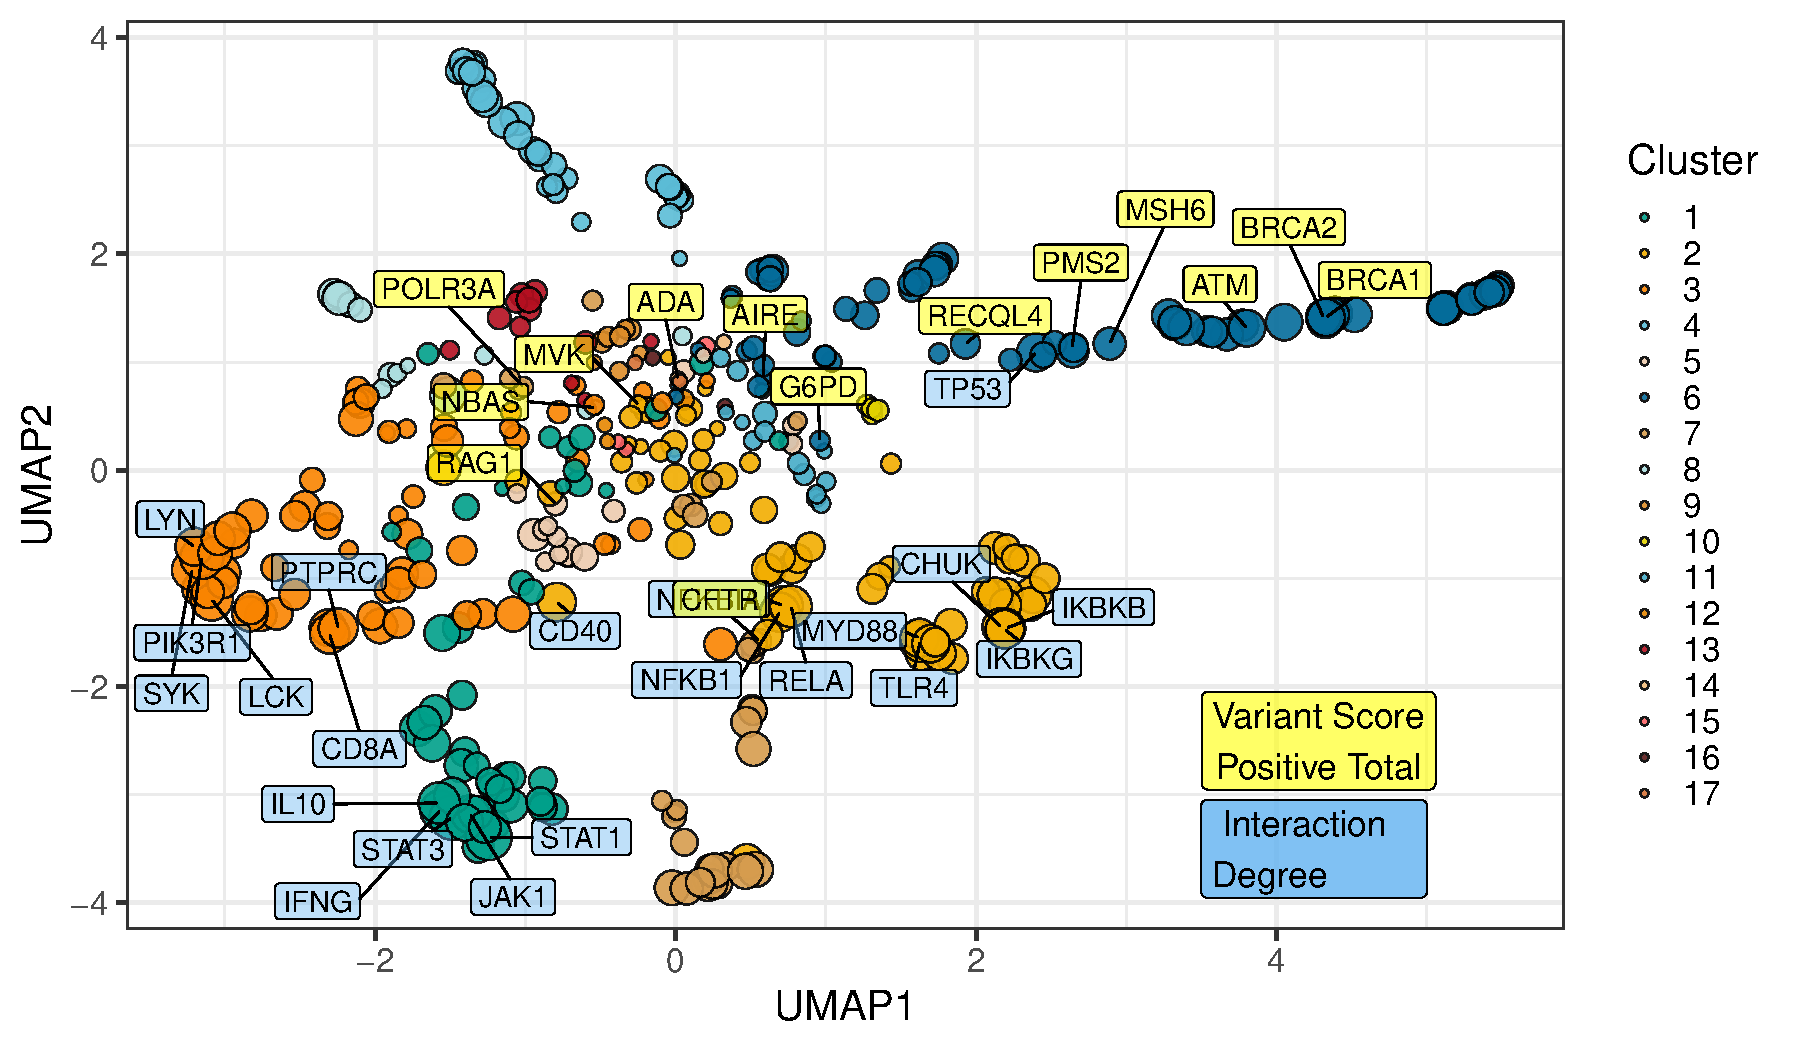
\includegraphics[width=0.99\textwidth]{../images/untangleR_ppi_network_umap.pdf}
  \caption{
    \textbf{\ac{umap} embedding of the \ac{ppi} network (p\_umap).} 
    The plot projects the high-dimensional protein-protein interaction network into two dimensions, with nodes coloured by cluster and sized by interaction degree. Blue labels indicate hub genes (degree above the 95th percentile) and yellow labels mark the top 15 genes by score positive total (damaging ClinVar classifications). The spatial segregation suggests that genes with high pathogenic variant loads are distinct from highly connected nodes.
  }
  \label{fig:p_umap}
\end{figure}

\FloatBarrier
\subsubsection{Hierarchical Clustering of Enrichment Scores for Major Disease Categories}
\textbf{Figure \ref{fig:patch2}} presents a heatmap of standardised residuals for major disease categories across network clusters, as per \textbf{Figure \ref{fig:p_umap}}. 
A dendrogram clusters similar disease categories, while the accompanying bar plot displays the maximum absolute standardised residual for each category.
Notably, (8) \ac{cd} shows the highest maximum enrichment, followed by 
(9) \ac{bmf}. 
While all maximum values exceed 2, the threshold for significance, this likely reflects the presence of protein clusters with strong damaging variant scores rather than uniform significance across all categories (i.e. genes from cluster 4 in 8 \ac{cd}).


\subsubsection{PPI Connectivity, LOEUF Constraint and Enriched Network Cluster Analysis}

Based on the preliminary insight from \textbf{Figure \ref{fig:patch2}} ,
we evaluated the relationship between network connectivity (\ac{ppi} degree) and \ac{lof} constraint (\ac{loeuf} upper rank) \citet{karczewski2020mutational} using Spearman’s rank correlation.
Overall, there was a weak but significant negative correlation ($\rho = -0.181$, $p = 0.00024$) at the global scale, indicating that highly connected genes tend to be more constrained. 
A supplementary analysis (\textbf{Figure \ref{fig:p_umap_const}})
did not reveal distinct visual associations between network clusters and constraint metrics, likely due to the high network density. 
However once stratified by gene clusters, the natural biological scenario based on quantitative \ac{ppi} evidence \cite{szklarczyk2025string},
some groups showed strong correlations; for instance, cluster 2 ($\rho = -0.375$, $p = 0.000994$) and cluster 4 ($\rho = -0.800$, $p < 0.000001$), while others did not.
This indicated that shared mechanisms within pathway clusters may underpin genetic constraints, particularity for \ac{lof} intolerance. We observe that the score positive total metric effectively summarises the aggregate pathogenic burden across \ac{iei} genes, serving as a robust indicator of genetic constraint and highlighting those with elevated disease relevance.

\begin{figure}[ht]
  \centering
  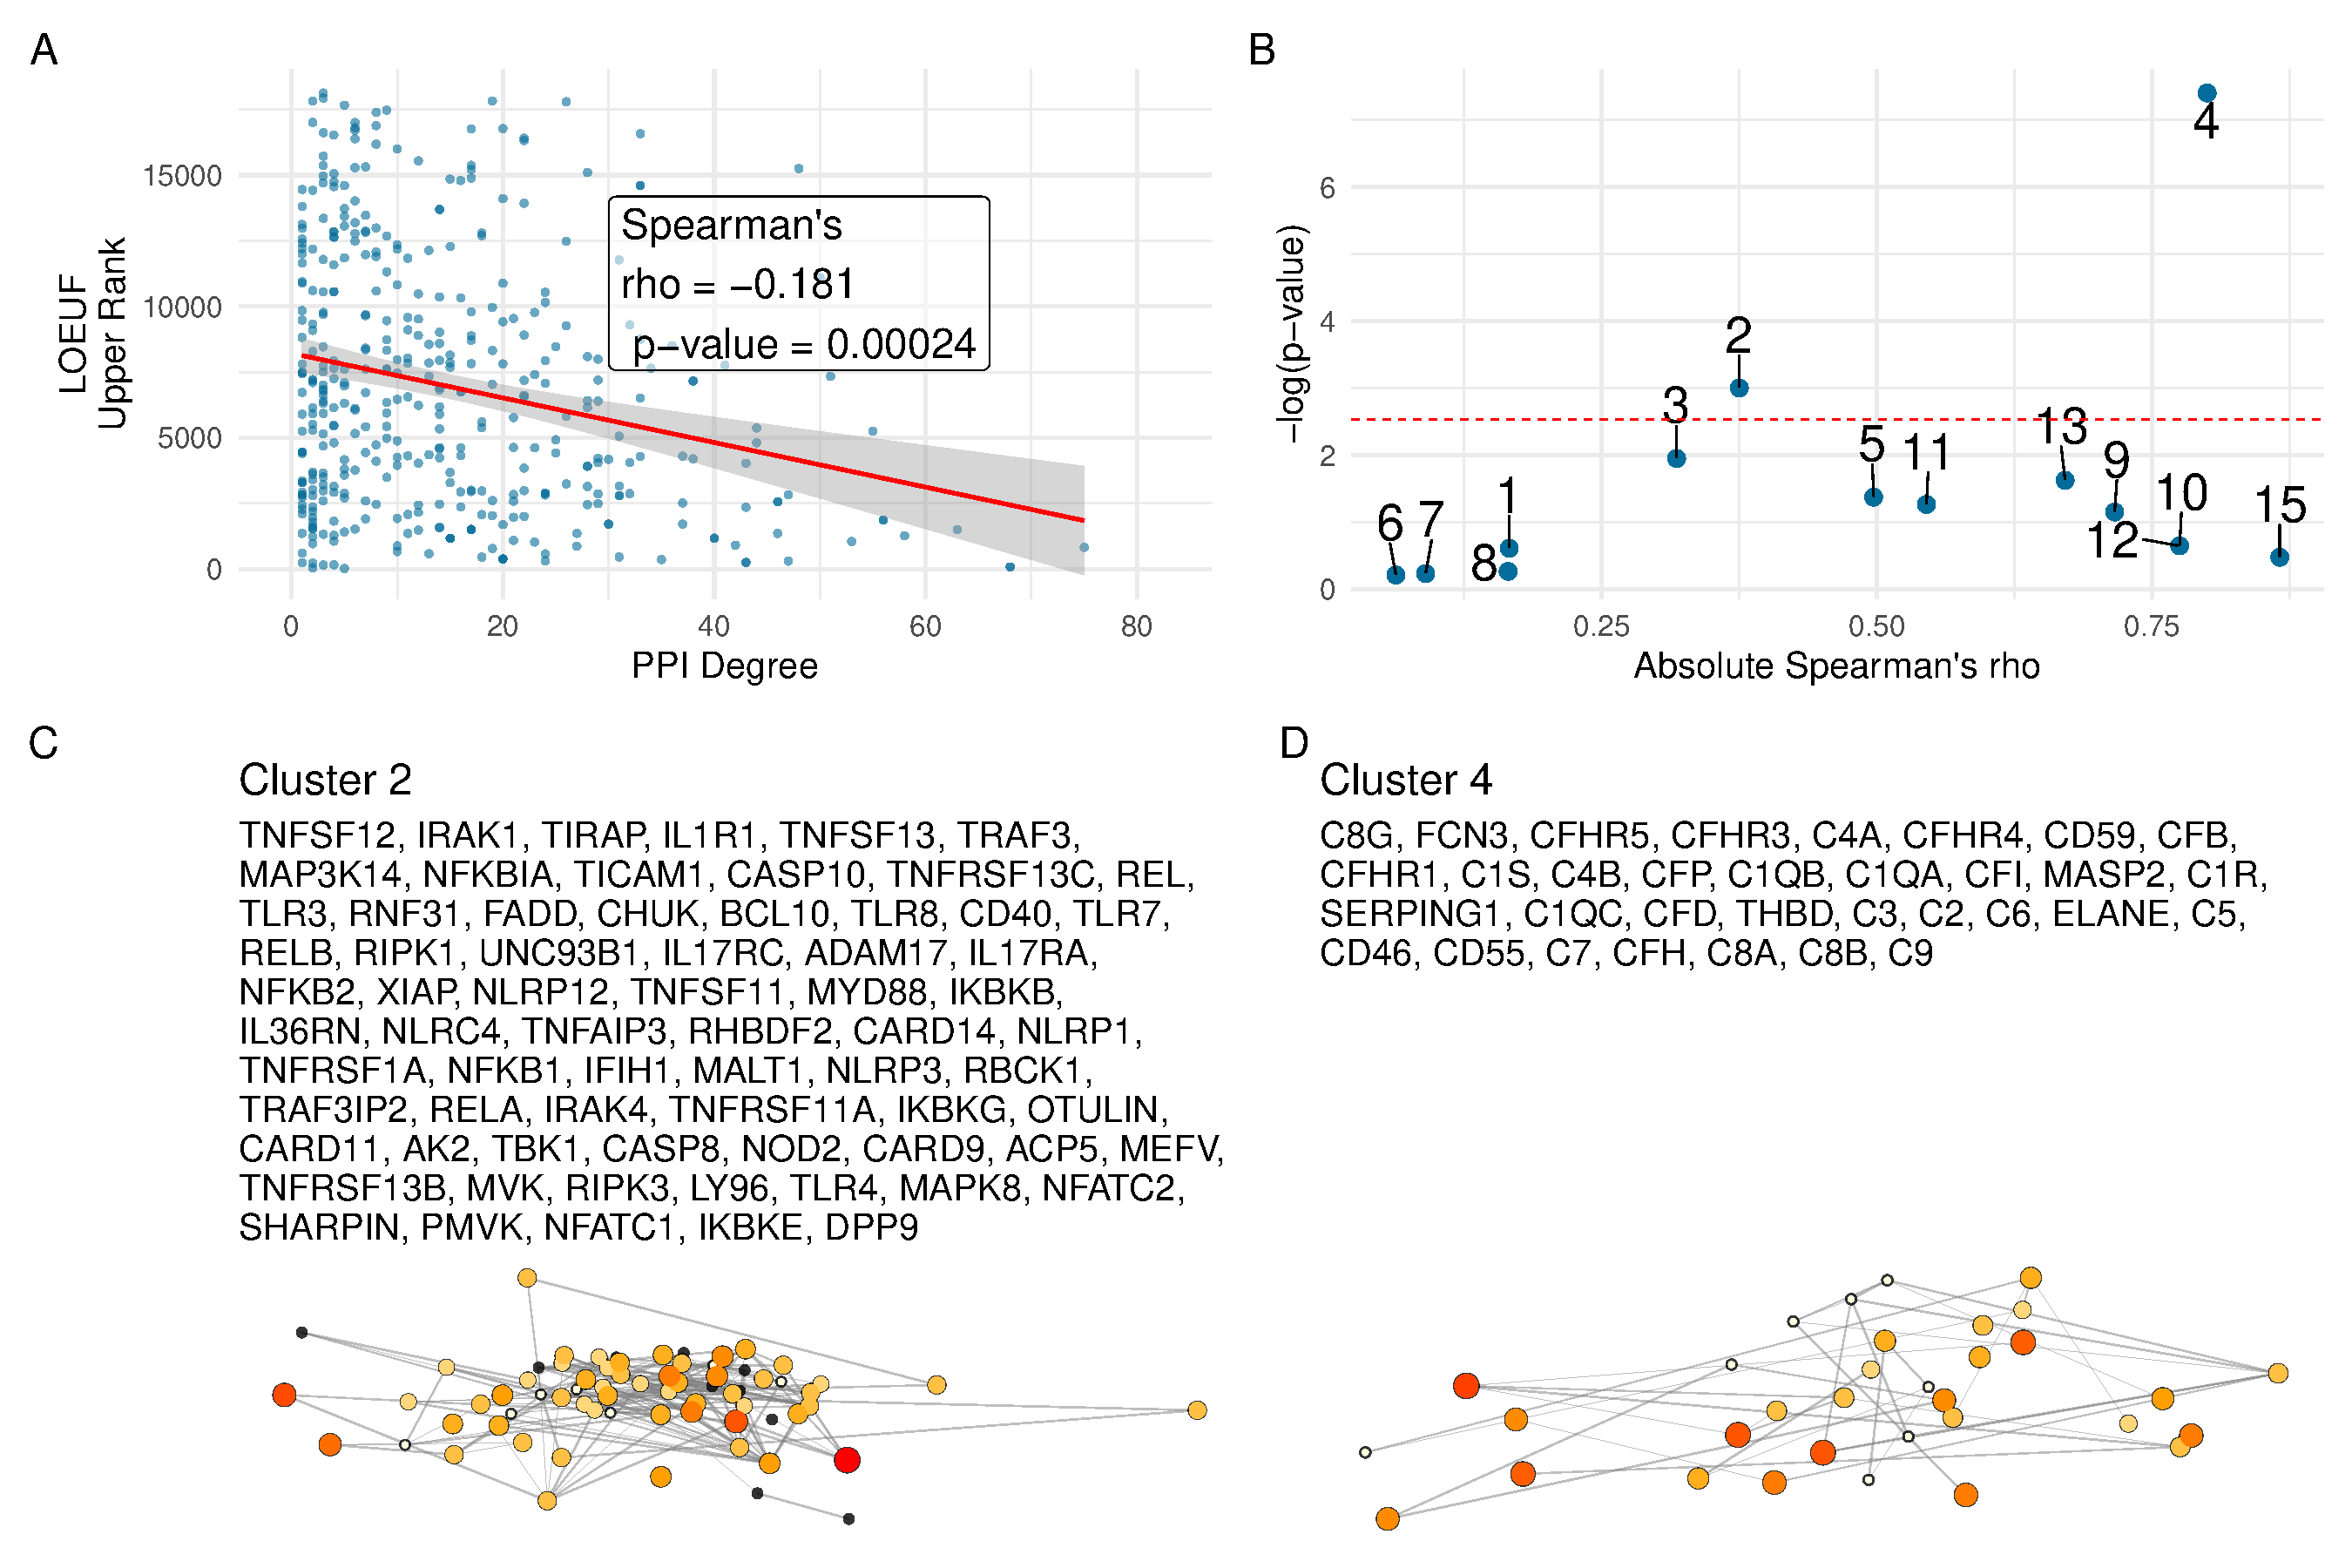
\includegraphics[width=0.99\textwidth]{../images/untangleR_ppi_network_p_cor_spear_rho_sig_clust_patch3.pdf}
  \caption{
    \textbf{Correlation between \ac{ppi} degree and \ac{loeuf} upper rank.} 
    \textbf{(A)} Ananlysis across all genes revealed a weak, significant negative correlation between \ac{ppi} degree and \ac{loeuf} upper rank. \textbf{(B)} The cluster-wise analysis showed that clusters 2 and 4 exhibited moderate to strong correlations, while other clusters display weak or non-significant relationships. \textbf{(C) and (D)} Shows the new network plots for the significantly enriched clusters based on \ac{gnomad} constraint metrics.
  }
  \label{fig:p_cor_spear_rho_sig_clust_patch3}
\end{figure}

% \subsubsection{Network Analysis of Enriched Significant Clusters Based on \ac{gnomad} Constraint}
\textbf{Figure \ref{fig:p_cor_spear_rho_sig_clust_patch3} (C, D)} shows the re-plotted \ac{ppi} networks for clusters with significant correlations between \ac{ppi} degree and \ac{loeuf} upper rank. In these networks, node size is scaled by a normalised variant score, while node colour reflects the variant score according to a predefined palette.

\subsection{New Insight from Functional Enrichment}
To interpret the functional relevance of our prioritised \ac{iei} gene sets with the highest load of damaging variants (i.e. clusters 2 and 4 in \textbf{Figure \ref{fig:p_cor_spear_rho_sig_clust_patch3}}), we performed functional enrichment analysis for known disease associations using MsigDB with FUMA (i.e. GWAScatalog and Immunologic Signatures) \cite{watanabe_functional_2017}. Composite enrichment profiles (\textbf{Figure \ref{fig:fuma_merge}}) reveal that our enriched \ac{ppi} clusters were associated with distinct disease-related phenotypes, providing functional insights beyond traditional \ac{iuis} \ac{iei} groupings \cite{tangye_human_2022}. The gene expression profiles shown in \textbf{Figure \ref{fig:expHeatmaps}} (GTEx v8 54 tissue types) offer the tissue-specific context for these associations. Together, these results enable the annotation of \ac{iei} gene sets with established disease phenotypes, supporting a data-driven classification of \ac{iei}.

Based on these independent sources of interpretation, we observed that genes from cluster 2 were independently associated with specific inflammatory phenotypes, including ankylosing spondylitis, psoriasis, inflammatory bowel disease, and rheumatoid arthritis, as well as quantitative immune traits such as lymphocyte and neutrophil percentages and serum protein levels.
In contrast, genes from Cluster 4 were linked to ocular and complement-related phenotypes, notably various forms of age-related macular degeneration (e.g. geographic atrophy and choroidal neovascularisation) and biomarkers of the complement system (e.g. C3, C4, and factor H-related proteins), with additional associations to nephropathy and pulmonary function metrics.

\subsection{Genome-wide Gene Distribution and Locus-specific Variant Occurrence}

\textbf{Figure \ref{fig:karyo_locusplot_merged} (A)} shows a genome-wide karyoplot of all \ac{iei} panel genes across GRCh38, with colour-coding based on \ac{moi}. Figures \textbf{(B)} and \textbf{(C)} display zoomed-in locus plots for \textit{NFKB1} and \textit{CFTR}, respectively. 
In \textbf{Figure \ref{fig:karyo_locusplot_merged} (B)}, the probability of observing variants with known classifications is high only for variants such as p.Ala475Gly, which are considered benign in the \ac{ad} \textit{NFKB1} gene that is intolerant to \ac{lof}. 
In \textbf{Figure \ref{fig:karyo_locusplot_merged} (C)}, high probabilities of observing patients with pathogenic variants in \textit{CFTR} are evident, reproducing this well-established phenomenon. Furthermore, the analysis of \ac{ld} using $\text{R}^2$ shows that high LD regions can be modelled effectively, allowing independent variant signals to be distinguished.

\begin{figure}[ht]
  \centering
  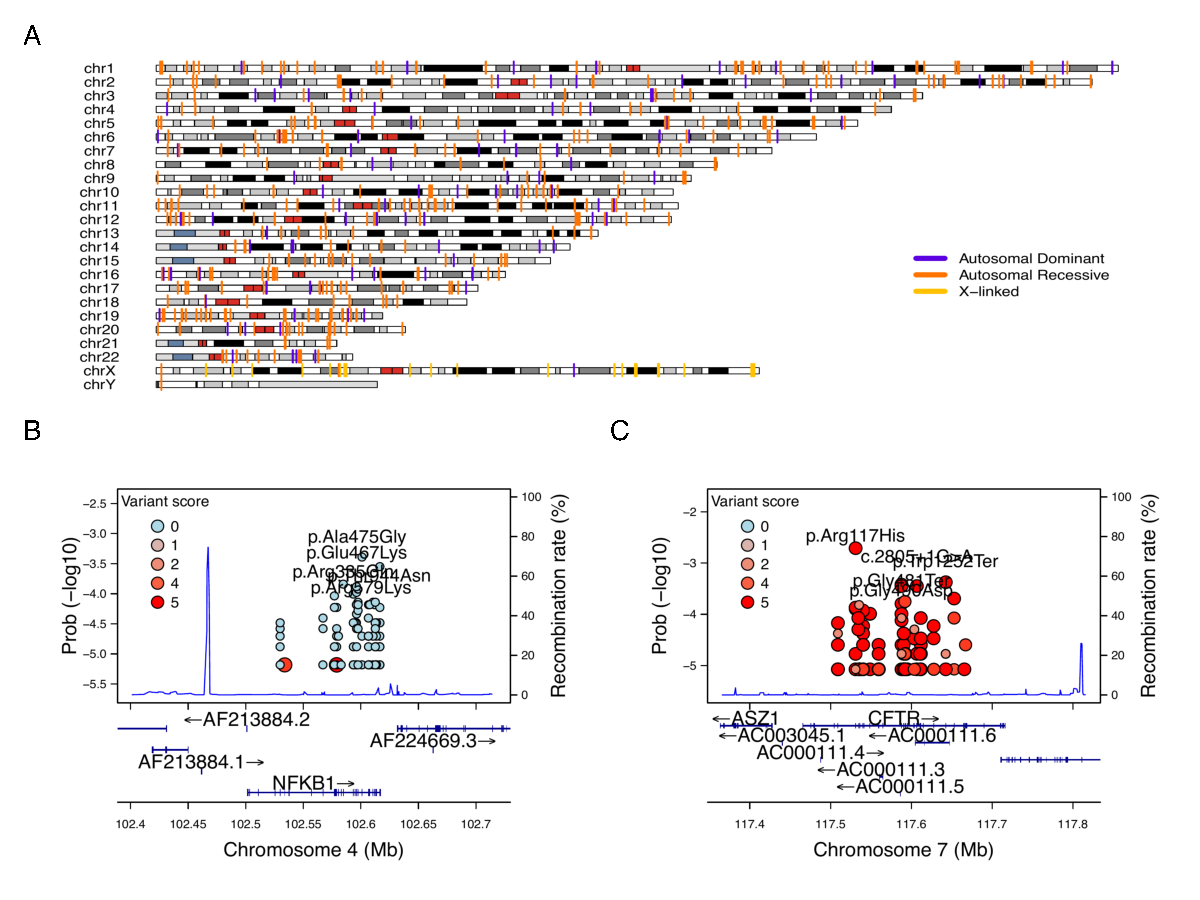
\includegraphics[width=0.99\textwidth]{../images/karyo_locusplot_merged.pdf}
  \caption{\textbf{Genome-wide \ac{iei}, variant occurance probability and \ac{ld} by $\text{R}^2$.} (A) Genome-wide karyoplot of all \ac{iei} panel genes mapped to GRCh38, with colours indicating \ac{moi}. (B) Zoomed-in locus plot for \textit{NFKB1} showing variant observation probabilities; only benign variants such exhibit high probabilities in this \ac{ad} gene intolerant to \ac{lof}. (C) Locus plot for \textit{CFTR} displaying high probabilities for pathogenic variants; due to the dense clustering of pathogenic variants, score filter >0 was applied. Top five variant are labelled per gene.}
  \label{fig:karyo_locusplot_merged}
\end{figure}

\subsection{Novel PID classifications derived from genetic PPI and clinical features}
%This section looks at the current 9 major IEI classes, and ~45 subclasses.
%These were designed over last few decades based on phenotype observation and subjective decisions.
%We can use the new information be potentially define better, new data-based classifications: clustering by PPI, severity/probability, and markers (T, B, NK, Ig), phenotype CVID, etc. 
We recategorised 315 immunophenotypic features from the original \ac{iuis} \ac{iei} annotations, reducing detailed descriptions (e.g. ``decreased cd8, normal or decreased cd4''), first to 
minimal labels (e.g.``low''), and second to binary outcomes (normal vs. not-normal) for T cells, B cells, neutrophils, and immunoglobulins (\textbf{Figure \ref{fig:immunophenotype_before_after}}). 
These simplified profiles were integrated with \ac{ppi} network clustering from STRINGdb to refine \ac{pid} gene groupings. 
Chi-square analyses confirmed significant associations between specific clinical abnormalities and \ac{ppi} clusters (\textbf{Figure \ref{fig:chi_heatmaps}}). 
A decision tree classifier, with hyperparameters optimised via 5-fold cross validation, demonstrated high sensitivity and specificity, as shown in the confusion matrices and variable importance metrics (\textbf{Figure \ref{fig:confusion_matrix}}). 
The resulting novel \ac{pid} classifications, illustrated by the decision tree and gene group distributions (\textbf{Figure \ref{fig:pid_class_tree_distribution}}), provide a more coherent and data-driven framework for categorising \ac{pid} genes.


\subsection{Novel PID classifications derived from genetic PPI and clinical features}
We recategorised 315 immunophenotypic features from the original \ac{iuis} \ac{iei} annotations, reducing detailed descriptions (e.g.\ “decreased CD8, normal or decreased CD4”) to minimal labels (e.g.\ “low”) and then binarising them (normal vs.\ not-normal) for T cells, B cells, \ac{ig} and neutrophils 
(\textbf{Figure \ref{fig:immunophenotype_before_after}}). 
These simplified profiles were mapped onto STRINGdb PPI clusters, revealing non‑random distributions ($\chi^2 < 1e‑13$; 
\textbf{Figure \ref{fig:plot_multicat_patch_3_clust_chi}}), indicating that network context captures key immunophenotypic variation.

We next compared four classifiers under 5‑fold cross‑validation to determine which features predicted PPI clustering.
As shown in \textbf{Figure \ref{fig:multicat_performance_combined}}, the fully combined model achieved the highest accuracy among the four:
(i) phenotypes only (33 \%) (i.e. T cell, B cell, \ac{ig}, Neutrophil);
(ii) phenotypes + IUIS major category (50 \%) (e.g. CID. See \textbf{Box \ref{box:definitions}} for more);
(iii) IUIS major + subcategory only (59 \%) (e.g. CID, T-B+ SCID); and
(iv) phenotypes + IUIS major + subcategory  (61 \%).
This demonstrated that incorporating both traditional IUIS classifications and core immunophenotypic markers into the PPI‑based framework yielded the most robust discrimination of PID gene clusters.
Variable importance analysis highlighted abnormality status for \ac{ig} and T cells
were among the top ten features in addition to the other IUIS major and sub categories. 
Per‑class specificity remained uniform across the classes while sensitivity dropped.

The PPI  and  immunophenotype model yielded 17 data‑driven PID groups, whereas incorporating the full complement of IUIS categories expanded this to 33 groups. 
For clarity, we only demonstrate the decision tree from the smaller 17‑group model in 
\textbf{Figure \ref{fig:pid_class_tree_distribution}}.
% full model: plot_multicat_combined_classification_tree.pdf
Each terminal node is annotated by its predominant immunophenotypic signature (for example, ``group 65 with abnormal T cell and B cell features''), and the full resulting gene counts per 33 class are plotted in 
% \textbf{Figure \ref{fig:multicat_new_pid_classes_combined}}. 
\textbf{Figure \ref{fig:pid_class_tree_distribution}}.
Although, less user-friendly, this data‑driven taxonomy 
both aligns with and refines traditional \ac{iuis} \ac{iei} classifications
%Although, less user-friendly, 
to provide a scaffold for large‑scale computational analyses.
Because this framework is fully reproducible, alternative PPI embeddings or incorporate additional molecular annotations can readily swapped to continue building on these PID classification schemes.

\begin{figure}[ht]
  \centering
  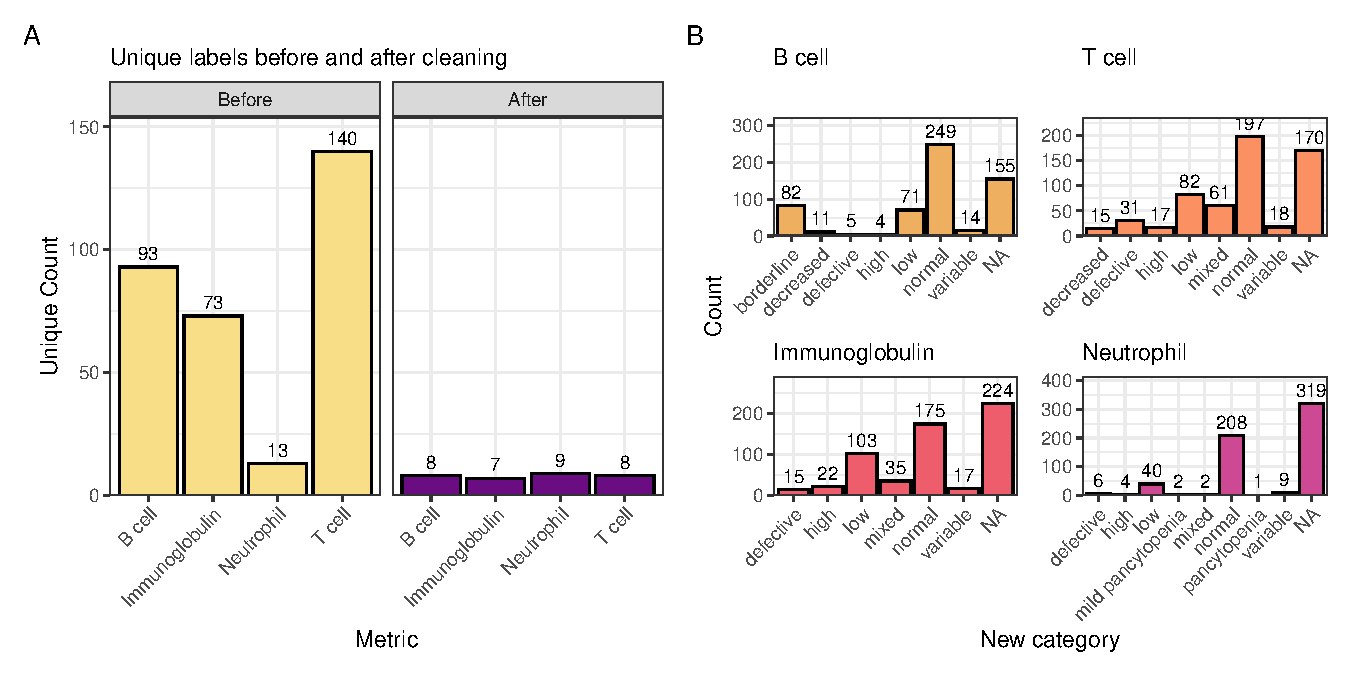
\includegraphics[width=0.99\textwidth]{../images/plot_patch1.pdf}
 %   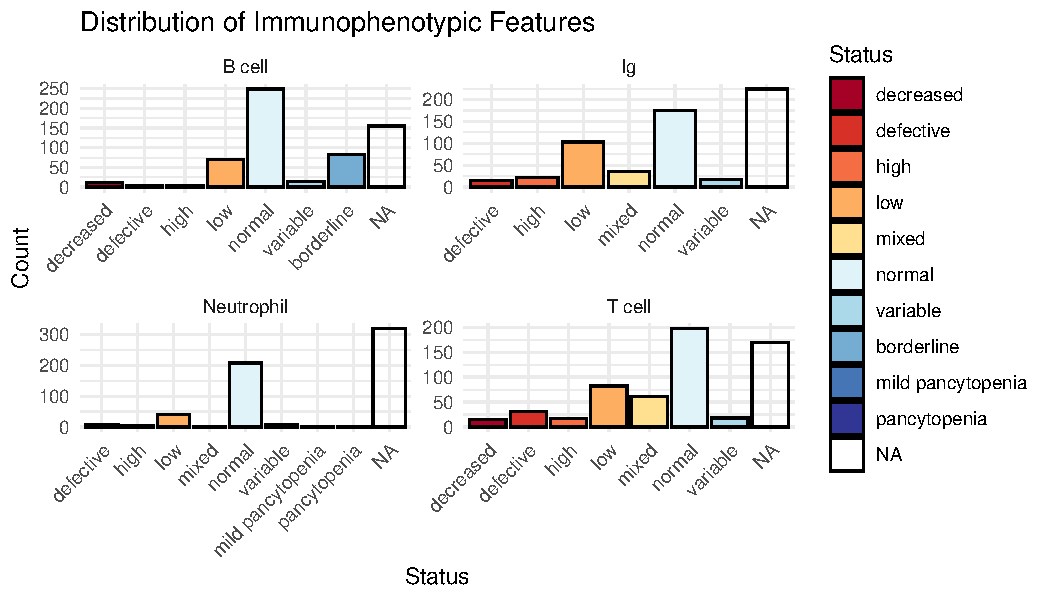
\includegraphics[width=0.7\textwidth]{../images/plot_patch_1_v2.pdf}
  \caption{ \textbf{Distribution of immunophenotypic features before and after recategorisation.}
  The original \ac{iuis} \ac{iei} descriptions contain information such as T cell-related
  ``decreased cd8, normal or decreased cd4 cells'' which we recategorise as ``low''.
  The bar plot shows the count of unique labels for each status (normal, not\_normal) across the T cell, B cell, \ac{ig}, and Neutrophil features.}
  \label{fig:immunophenotype_before_after}
\end{figure}

\begin{figure}[ht]
  \centering
  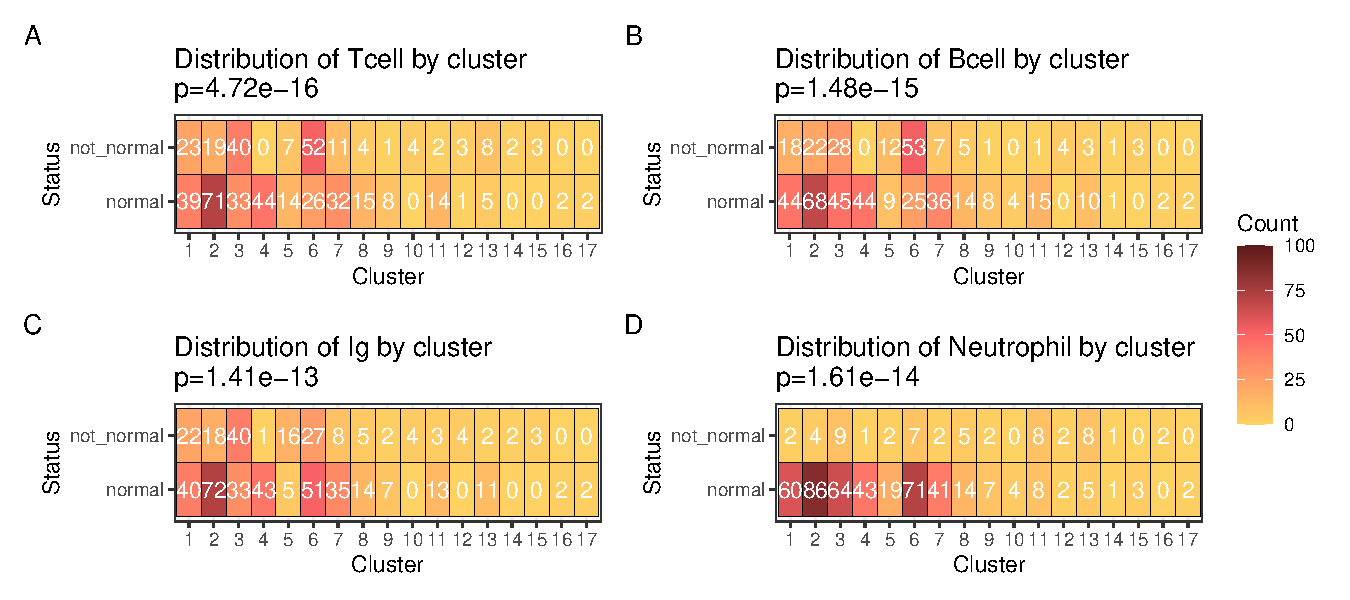
\includegraphics[width=0.99\textwidth]{../images/plot_multicat_patch_3_clust_chi.pdf}
  \caption{\textbf{Heatmaps of clinical feature distributions by PPI cluster.} The heatmaps display the count of observations for abnormality of each clinical feature (A) T cell, (B) B cell, (C) Immunoglobulin, (D) Neutrophil, in relation to the PPI clusters, with p-values from chi-square tests annotated in the titles.}
  \label{fig:plot_multicat_patch_3_clust_chi}
\end{figure}

\begin{figure}[ht]
  \centering
  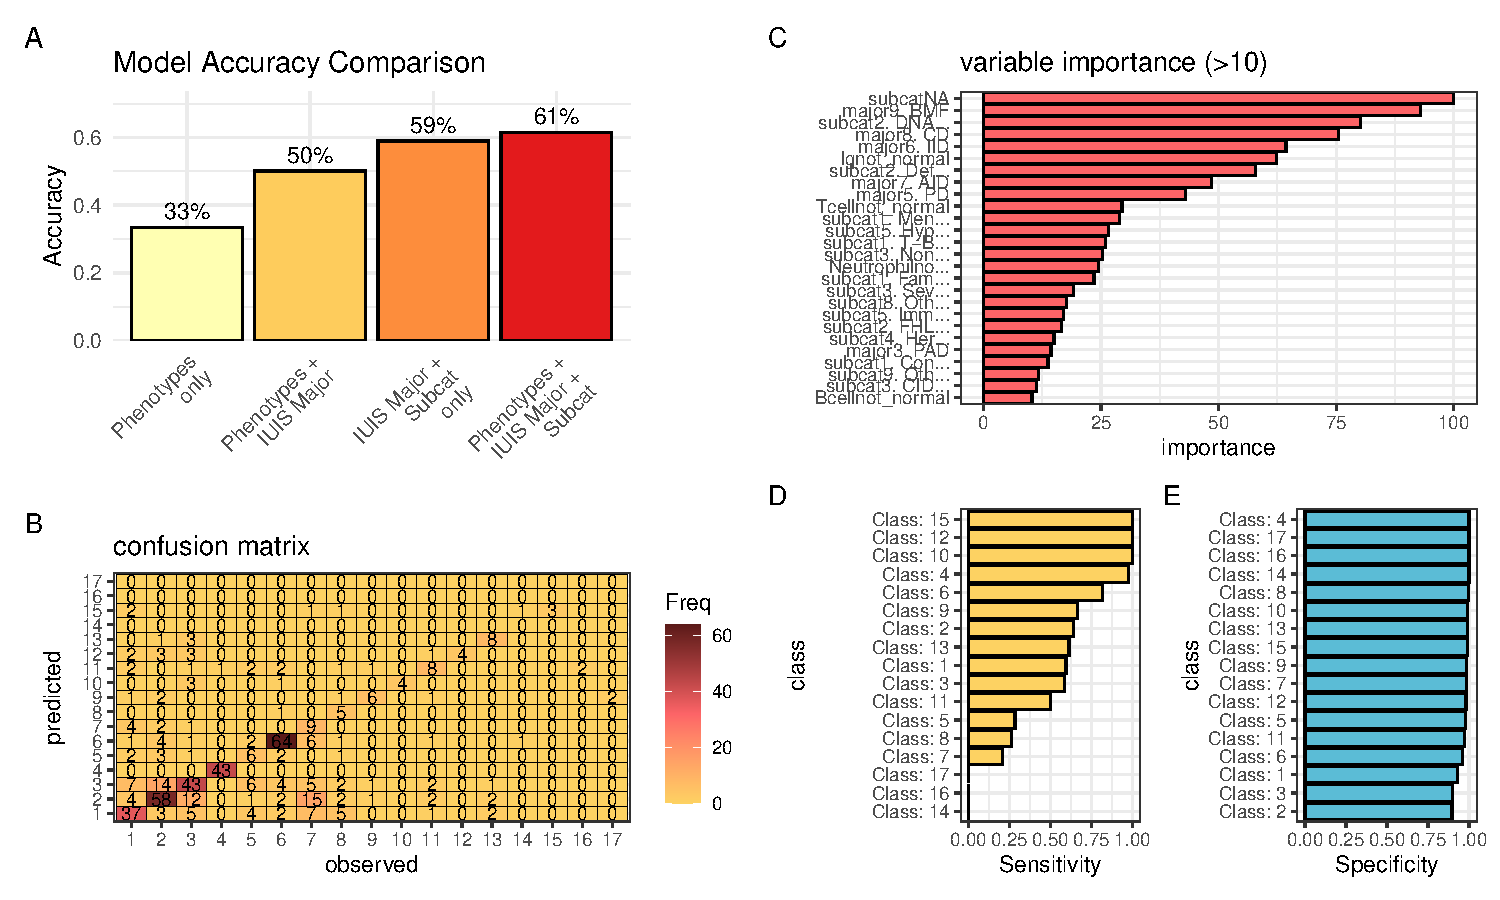
\includegraphics[width=0.99\textwidth]{../images/plot_multicat_performance_combined.pdf}
  \caption{\textbf{Performance comparison of PID classifiers.} Classification predicting PPI cluster membership from IUIS major category, subcategory, and immunological features. (A) Overall accuracy for four rpart models
used to predict \ac{ppi} clustering. The combined model achieves 61.4 \% accuracy, exceeding all simpler approaches. 
Nodes were split to minimize Gini impurity, pruned by cost-complexity (cp = 0.001), and validated via 5‑fold cross‑validation. %Terminal leaves display the assigned cluster and the proportion of genes falling into each group. 
(B-E) The summary statistics from the top model are detailed.  
}
  \label{fig:multicat_performance_combined}
\end{figure}

\begin{figure}[ht]
  \centering
  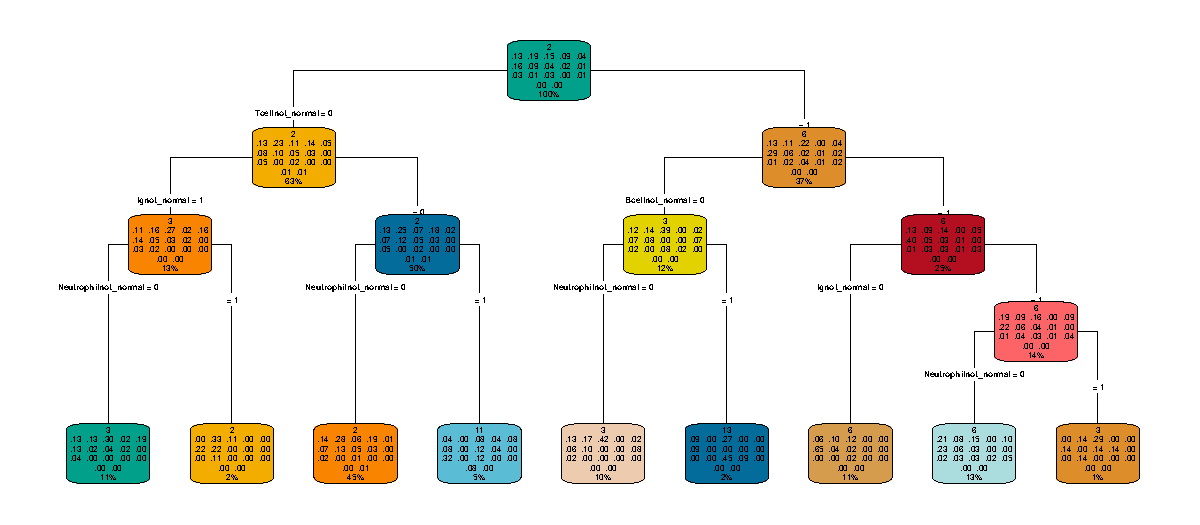
\includegraphics[width=0.99\textwidth]{../images/p_new_classification_finetune_tree.pdf}       
  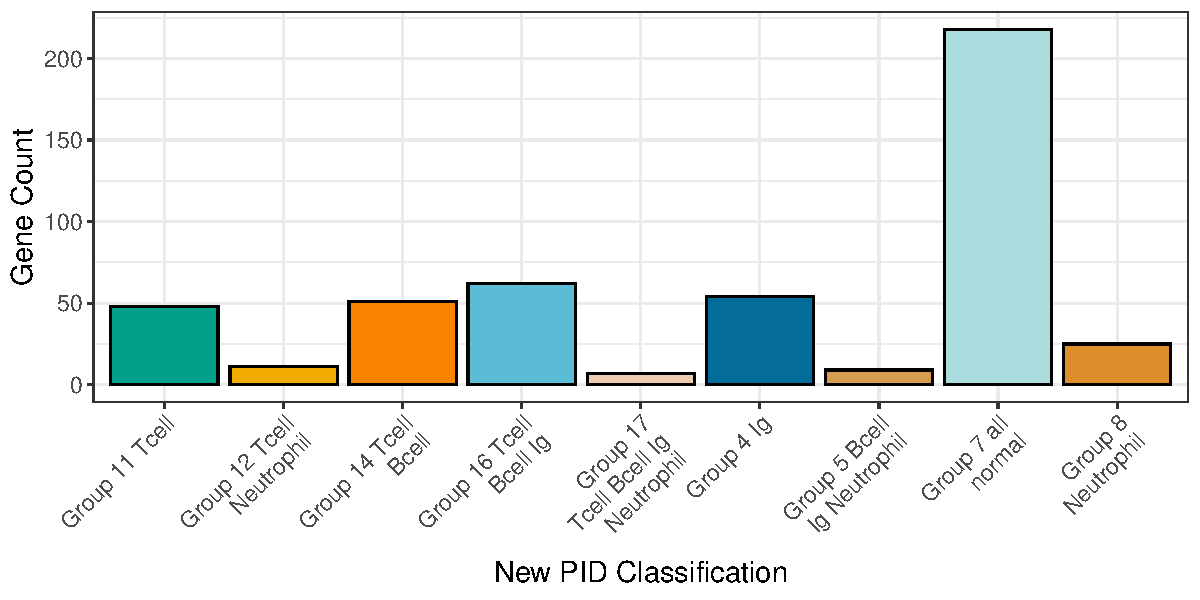
\includegraphics[width=0.99\textwidth]{../images/plot_new_pid_classifications_genetic.pdf}
  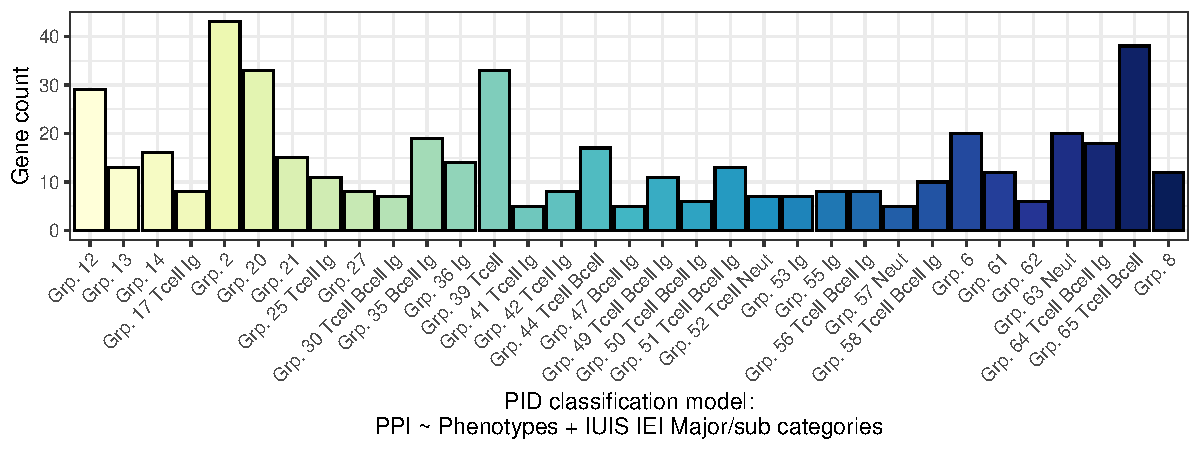
\includegraphics[width=0.99\textwidth]{../images/plot_multicat_new_pid_classes_combined.pdf}
  \caption{\textbf{ Fine-tuned model for PID classification.} 
  (Top) In each terminal node, the top block indicates the number of genes in the node; the middle block shows the fitted class probabilities (which sum to 1); and the bottom block displays the percentage of the total sample in that node. These metrics summarise the model's assignment based on immunophenotypic and PPI features. (Middle) Bar plot presenting the distribution of novel PID classifications, where group labels denote the predominant abnormal clinical feature(s) (e.g. T cell, B cell, Ig, Neutrophil) characterising each group. (Bottom) The complete model including the traditional \ac{iuis} \ac{iei} categories.}  
  \label{fig:pid_class_tree_distribution}
\end{figure}

\FloatBarrier
\subsubsection{Integration of Variant Probabilities into IEI Genetics Data}
We integrated the computed prior probabilities for observing variants in all known genes associated with a given phenotype \cite{tangye_human_2022}, across \ac{ad}, \ac{ar}, and \ac{xl} \ac{moi}, into our \ac{iei} genetics framework. These calculations, derived from gene panels in PanelAppRex, have yielded novel insights for the \ac{iei} disease panel. The final result comprised of machine- and human-readable datasets, including the table of variant classifications and priors available via a the linked repository \cite{lawless_2025_15111584}, and a user-friendly web interface that incorporates these new metrics.

\textbf{Figure \ref{fig:var_risk_est_iei_genetics}} shows the interface summarising integrated variant data. Server-side pre-calculation of summary statistics minimises browser load, while clinical significance is converted to numerical metrics. Key quantiles (min, Q1, median, Q3, max) for each gene are rendered as sparkline box plots, and dynamic URLs link table entries to external databases (e.g. ClinVar, \ac{omim}, AlphaFold).

\begin{figure}[ht]
  \centering
  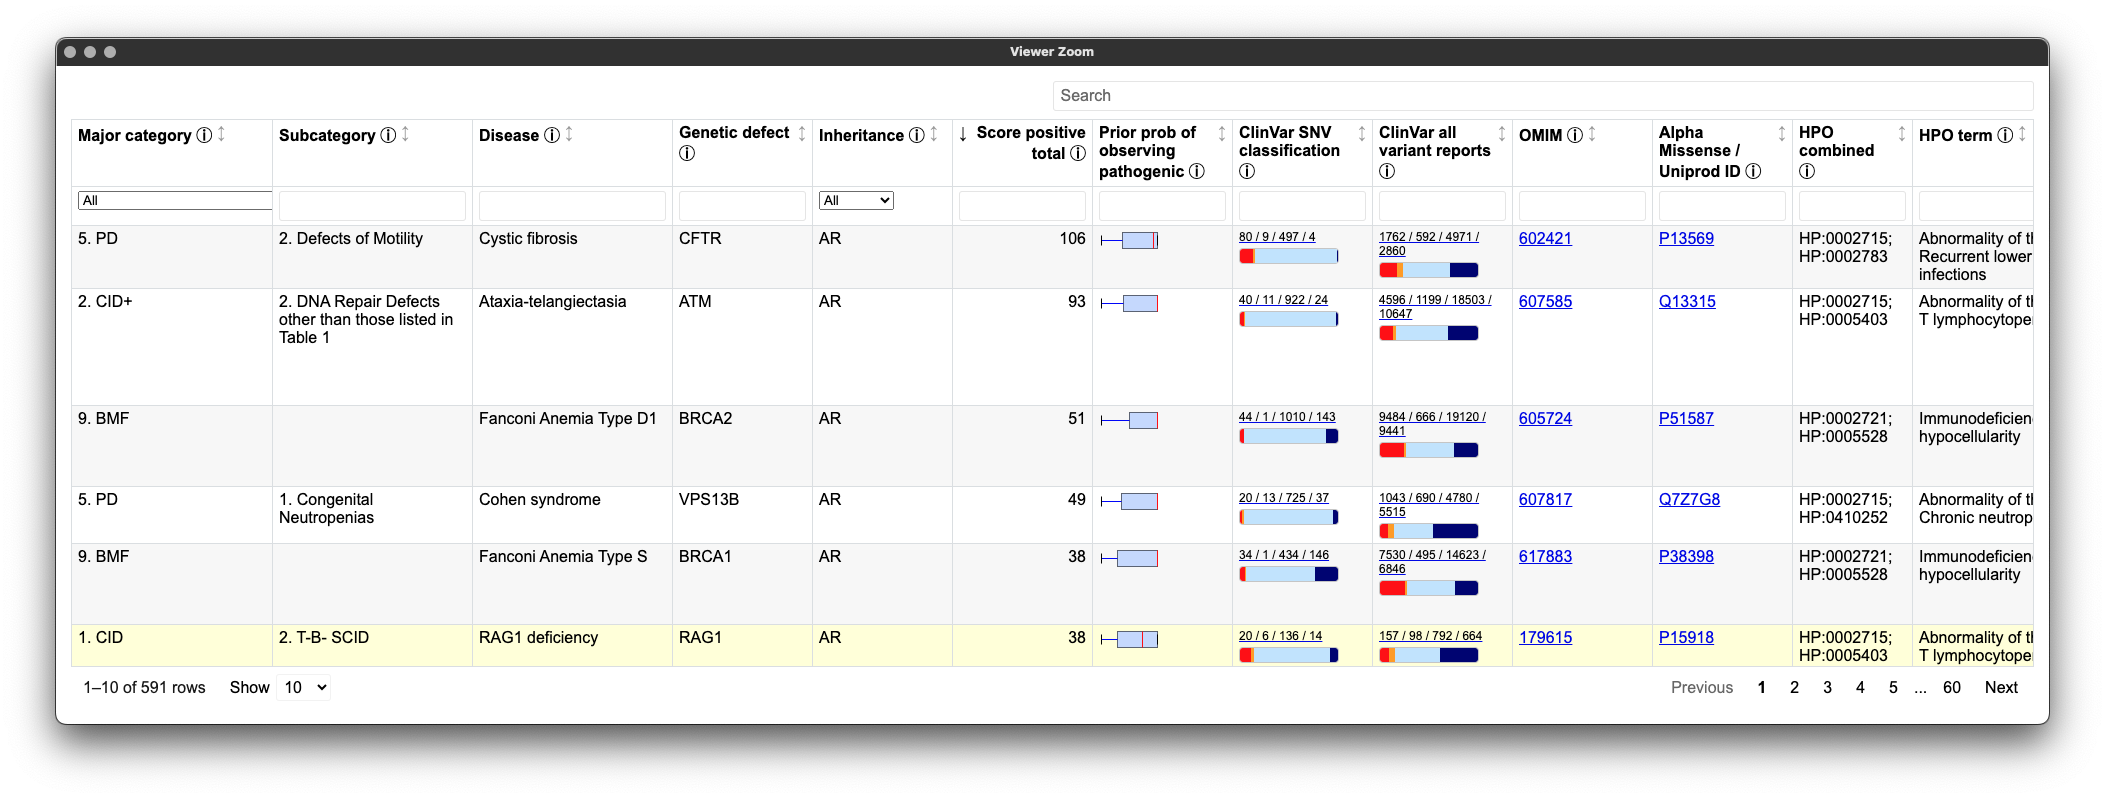
\includegraphics[width=1\textwidth]{../images/var_risk_est_iei_genetics.png}
  \caption{
    \textbf{Integration of variant probabilities into the \ac{iei} genetics framework.}
    The interface summarises the condensed variant data, with pre-calculated summary statistics and dynamic links to external databases. This integration enables immediate access to detailed variant classifications and prior probabilities for each gene.
  }
  \label{fig:var_risk_est_iei_genetics}
\end{figure}

\subsection{Probability of observing AlphaMissense pathogenicity}
AlphaMissense provides pathogenicity scores for all possible amino acid substitutions; however, our results in \textbf{Figure \ref{fig:alphamissense}} show that the most probable observations in patients occur predominantly for benign or unknown variants. This finding places the likelihood of disease-associated substitutions into perspective and offers a data-driven foundation for future improvements in variant prediction. The values in 
\textbf{Figure \ref{fig:alphamissense} (A)} can be directly compared to 
\textbf{Figure \ref{fig:p_varRisEst_summary_scores} (D)} to view the distribution of classifications.
A Kruskal-Wallis test was used to compare the observed disease probability across clinical classification groups and no significant differences were detected. In general, most variants in patients are classified as benign or unknown, indicating limited discriminative power in the current classification, such that pathogenicity prediction does not infer observation prediction (\textbf{Figure \ref{fig:alphamissense_kw}}).
  
\begin{figure}[ht]
\begin{center}
%    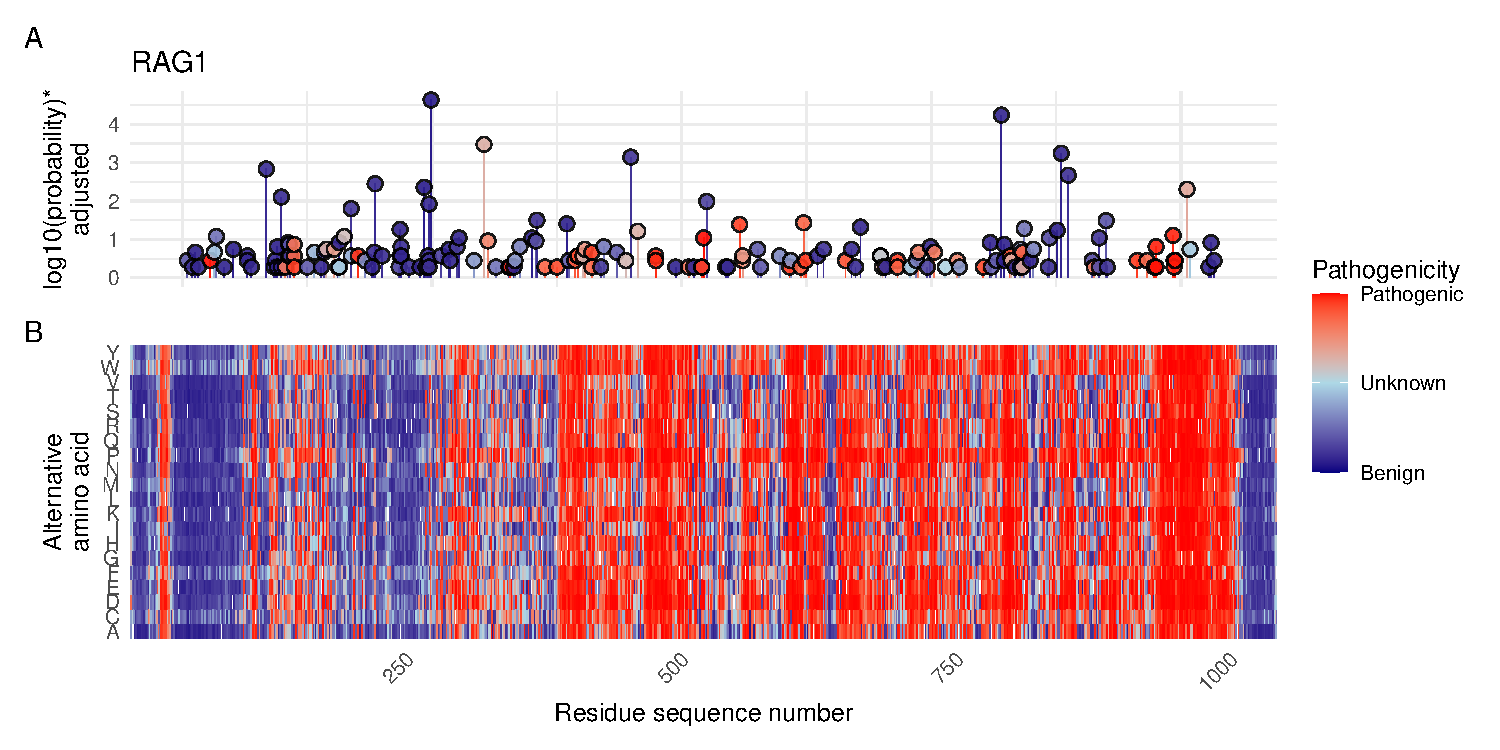
\includegraphics[width=0.99\textwidth]{../images/p_alphamissense_RAG1.pdf}
    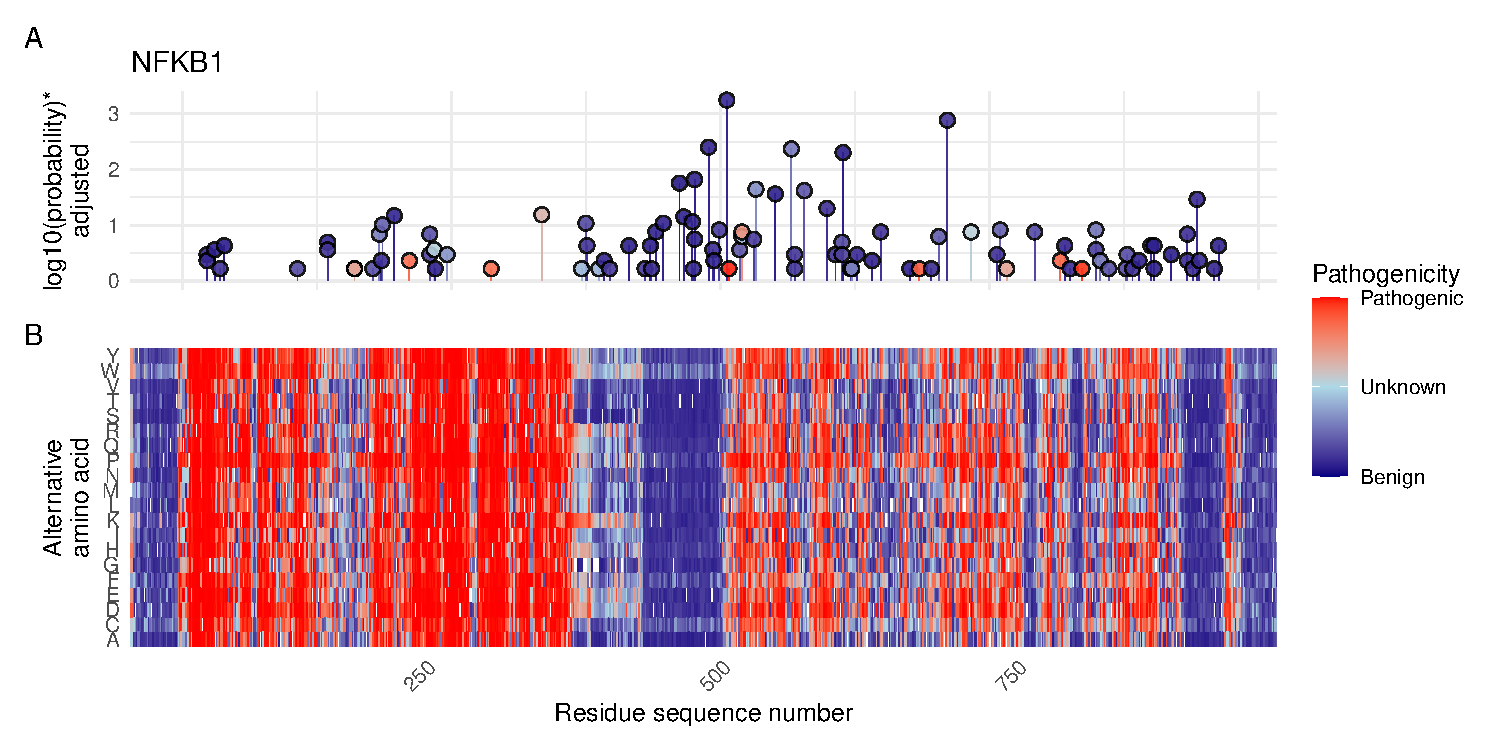
\includegraphics[width=0.85\textwidth]{../images/p_alphamissense_NFKB1.pdf}
    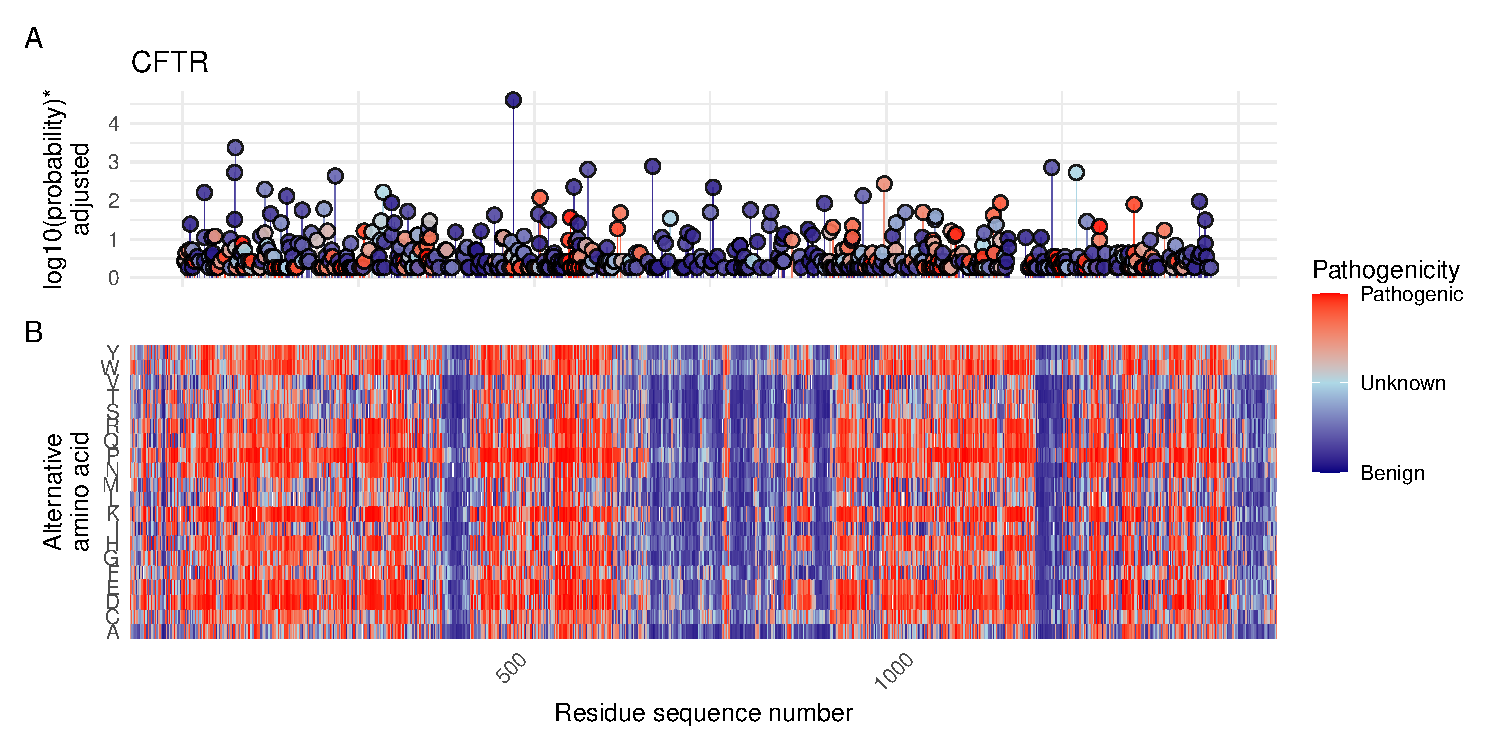
\includegraphics[width=0.85\textwidth]{../images/p_alphamissense_CFTR.pdf}
\end{center}
\caption{\textbf{(A) Probabilities of observing a patient with (B) AlphaMissense-derived pathogenicity scores.} Although AlphaMissense provides scores for every possible amino acid substitution, the most frequently observed variants in patients tend to be classified as benign or of unknown significance. This juxtaposition contextualises the likelihood of disease-associated substitutions and underlines prospects for refining predictive models. *Axis scaled for visibility near zero. Higher point indicates higher probability.}
 \label{fig:alphamissense}
\end{figure}

\FloatBarrier
\section{Discussion}

Our study presents, to our knowledge, the first comprehensive framework for calculating prior probabilities of observing disease-associated variants. By integrating large-scale genomic annotations, including population allele frequencies from \ac{gnomad} \cite{karczewski2020mutational}, variant classifications from ClinVar \cite{landrum_clinvar_2018}, and functional annotations from resources such as \ac{dbnsfp}, with classical Hardy-Weinberg-based calculations, we derived robust estimates for 54,814 ClinVar variant classifications across 557 \ac{iei} genes implicated in \ac{pid} and monogenic inflammatory bowel disease \cite{lawless_panelapprex_2025, tangye_human_2022}.

Our approach yielded two key results. First, our detailed, per-variant pre-calculated results provide prior probabilities of observing disease-associated variants across all \ac{moi} for any gene-disease combination. Second, the score positive total metric effectively summarises the aggregate pathogenic burden across genes, serving as a robust indicator of genetic constraint and highlighting those with elevated disease relevance.

Estimating disease risk in genetic studies is complicated by uncertainties in key parameters such as variant penetrance and the fraction of cases attributable to specific variants \cite{zschocke_mendelian_2023}. 
In the simplest model, where a single, fully penetrant variant causes disease, the lifetime risk \(P(D)\) is equivalent to the genotype frequency \(P(G)\). 
For an allele with frequency \(p\), this translates to:
\[
\begin{aligned}
\text{Recessive:} \quad P(D) &= p^2, \\
\text{Dominant:} \quad P(D) &= 2p(1-p) \approx 2p.
\end{aligned}
\]
When penetrance is incomplete, defined as \(P(D\mid G)\), the risk becomes:
\[
P(D) = P(G)\,P(D\mid G).
\]
In more realistic scenarios where multiple variants contribute to disease, \(P(G\mid D)\) denotes the fraction of cases attributable to a given variant. This leads to:
\[
P(D) = \frac{P(G)\,P(D\mid G)}{P(G\mid D)}.
\]
Because both penetrance and \(P(G\mid D)\) are often uncertain, solving this equation systematically poses a major challenge.

Our framework addresses this challenge by combining variant classifications, population allele frequencies, and curated gene-disease associations. 
%Although variant classifications are not perfect on an individual level, rigorous filtering based on empirical evidence ensures that only variants with confirmed pathogenicity—and thus more predictable penetrance—are included. 
While imperfect on an individual level, these sources exhibit predictable aggregate behaviour, supported by James-Stein estimation principles \cite{efron_steins_1973}.
% Keep this thought here: Stein's Estimation Rule and its competitors, as discussed by Efron and Morris (1973), demonstrate that shrinkage estimators—such as the James–Stein estimator—can outperform traditional maximum likelihood methods by “borrowing strength” across multiple parameters. In essence, even if individual estimates are noisy or imprecise, shrinking them towards a common value (or mean) improves the overall risk (mean squared error) of the estimates. This empirical Bayes approach shows that aggregate estimates tend to be well-calibrated, a principle we leverage in our work: although individual ClinVar variant classifications may be uncertain, their collective behaviour yields robust and reliable prior probabilities when combined with population allele frequencies and curated gene–disease associations.
Curated gene-disease associations help identify genes that explainable for most disease cases, allowing us to approximate \(P(G\mid D)\) close to one. In this way, we obtain robust estimates of \(P(G)\) (the frequency of disease-associated genotypes), even when exact values of penetrance and case attribution remain uncertain.

This approach allows us to pre-calculate priors and summarise the overall pathogenic burden using our \emph{score positive total} metric. By focusing on a subset \(\mathcal{V}\) of variants that pass stringent filtering, where each \(P(G_i \mid D)\) is the probability that a case of disease \(D\) is attributable to variant \(i\), we assume that, in aggregate,
\[
\sum_{i\in\mathcal{V}} P(G_i\mid D) \approx 1.
\]
% Definitions:
% \(\mathcal{V}\): the set of variants that pass our stringent filtering criteria based on empirical evidence.
% \(P(G_i \mid D)\): the probability that a disease case harbours the disease‐causing genotype corresponding to variant \(i\), given that the disease \(D\) is observed.
% \(D\): the disease state or condition.
% The expression \(\sum_{i\in\mathcal{V}} P(G_i\mid D) \approx 1\) implies that, in aggregate, the selected variants in \(\mathcal{V}\) account for nearly all cases of the disease.
Even if the cumulative contribution is slightly less than one, the resultant risk estimates remain robust within the broad confidence intervals typical of epidemiological studies. By incorporating these pre-calculated priors into a Bayesian framework, our method refines risk estimates and enhances clinical decision-making despite inherent uncertainties.

Our results focused on \ac{iei}, but the genome-wide approach accommodates the distinct \ac{moi} patterns of \ac{ad}, \ac{ar}, and \ac{xl} disorders. Whereas \ac{ad} and \ac{xl} conditions require only a single pathogenic allele, \ac{ar} disorders necessitate the consideration of both homozygous and compound heterozygous states. These classical \ac{hwe}-based estimates provide an informative baseline for predicting variant occurrence and serve as robust priors for Bayesian models of variant and disease risk estimation. This is an approach that has been underutilised in clinical and statistical genetics. As such, our framework refines risk calculations by incorporating \ac{moi} complexities and enhances clinicians’ understanding of expected variant occurrences, thereby improving diagnostic precision.

Moreover, our method complements existing statistical approaches for aggregating variant effects with methods like \ac{skat} and \ac{acat} \cite{liu2019acat,li2020dynamic,wu2011rare,lee2012optimal}) and multi-omics integration techniques \cite{kong2018nature,howe2021within}, while remaining consistent with established variant interpretation guidelines from the \ac{acmg} \cite{richards2015standards} and complementary frameworks \cite{tavtigian2020fitting,li2017intervar}, as well as quality control protocols \cite{pedersen2021effective,anderson2010data}. Standardised reporting for qualifying variant sets, such as \ac{acmg} Secondary Findings v3.2 \cite{miller2023acmg}, further contextualises the integration of these probabilities into clinical decision-making.

We acknowledge that our current framework is restricted to \ac{snv}s and does not incorporate numerous other complexities of genetic disease, such as structural variants, de novo variants, hypomorphic alleles, overdominance, variable penetrance, tissue-specific expression, the Wahlund effect, pleiotropy, and others \cite{zschocke_mendelian_2023}. In certain applications, more refined estimates would benefit from including factors such as embryonic lethality, condition-specific penetrance, and age of onset \cite{hannah_using_2024}. Our analysis also relies on simplifying assumptions of random mating, an effectively infinite population, and the absence of migration, novel mutations, or natural selection.

Future work will incorporate additional variant types and models to further refine these probability estimates. By continuously updating classical estimates with emerging data and prior knowledge, we aim to enhance the precision of genetic diagnostics and ultimately improve patient care.

\section{Conclusion}
Our work generates prior probabilities for observing any variant classification in \ac{iei} genetic disease, providing a quantitative resource to enhance Bayesian variant interpretation and clinical decision-making.

\section*{Acknowledgements}
\noindent
We acknowledge Genomics England for providing public access to the PanelApp data.
The use of data from Genomics England panelapp was licensed under the Apache License 2.0.
The use of data from \ac{uniprot} was licensed under Creative Commons Attribution 4.0 International (CC BY 4.0).
ClinVar asks its users who distribute or copy data to provide attribution to them as a data source in publications and websites \cite{landrum_clinvar_2018}.
\ac{dbnsfp} version 4.4a is licensed under the Creative Commons Attribution-NonCommercial-NoDerivatives 4.0 International (CC BY-NC-ND 4.0); while we cite this dataset as used our research publication, it is not used for the final version which instead used ClinVar and \ac{gnomad} directly.
GnomAD is licensed under  Creative Commons  Zero Public Domain Dedication (CC0 1.0 Universal).
GnomAD request that usages cites the \ac{gnomad} flagship paper \cite{karczewski2020mutational}
and any online resources that include the data set provide a link to the browser, and note that tool includes data from the \ac{gnomad} v4.1 release.
AlphaMissense asks to cite \citet{cheng_accurate_2023} for usage in research, with data available from \citet{jun_cheng_2023_8208688}.

\section*{Competing interest}
\noindent
We declare no competing interest. 

% \newpage
\bibliographystyle{unsrtnat}
\bibliography{references}

\clearpage
%\\\\\\\\\\\\\\\\\\\\\\\\\\\\
\beginsupplement
\section{Supplemental} \label{Supplemental_text}

\subsection{Validation studies}

\begin{figure}[ht]
  \centering
  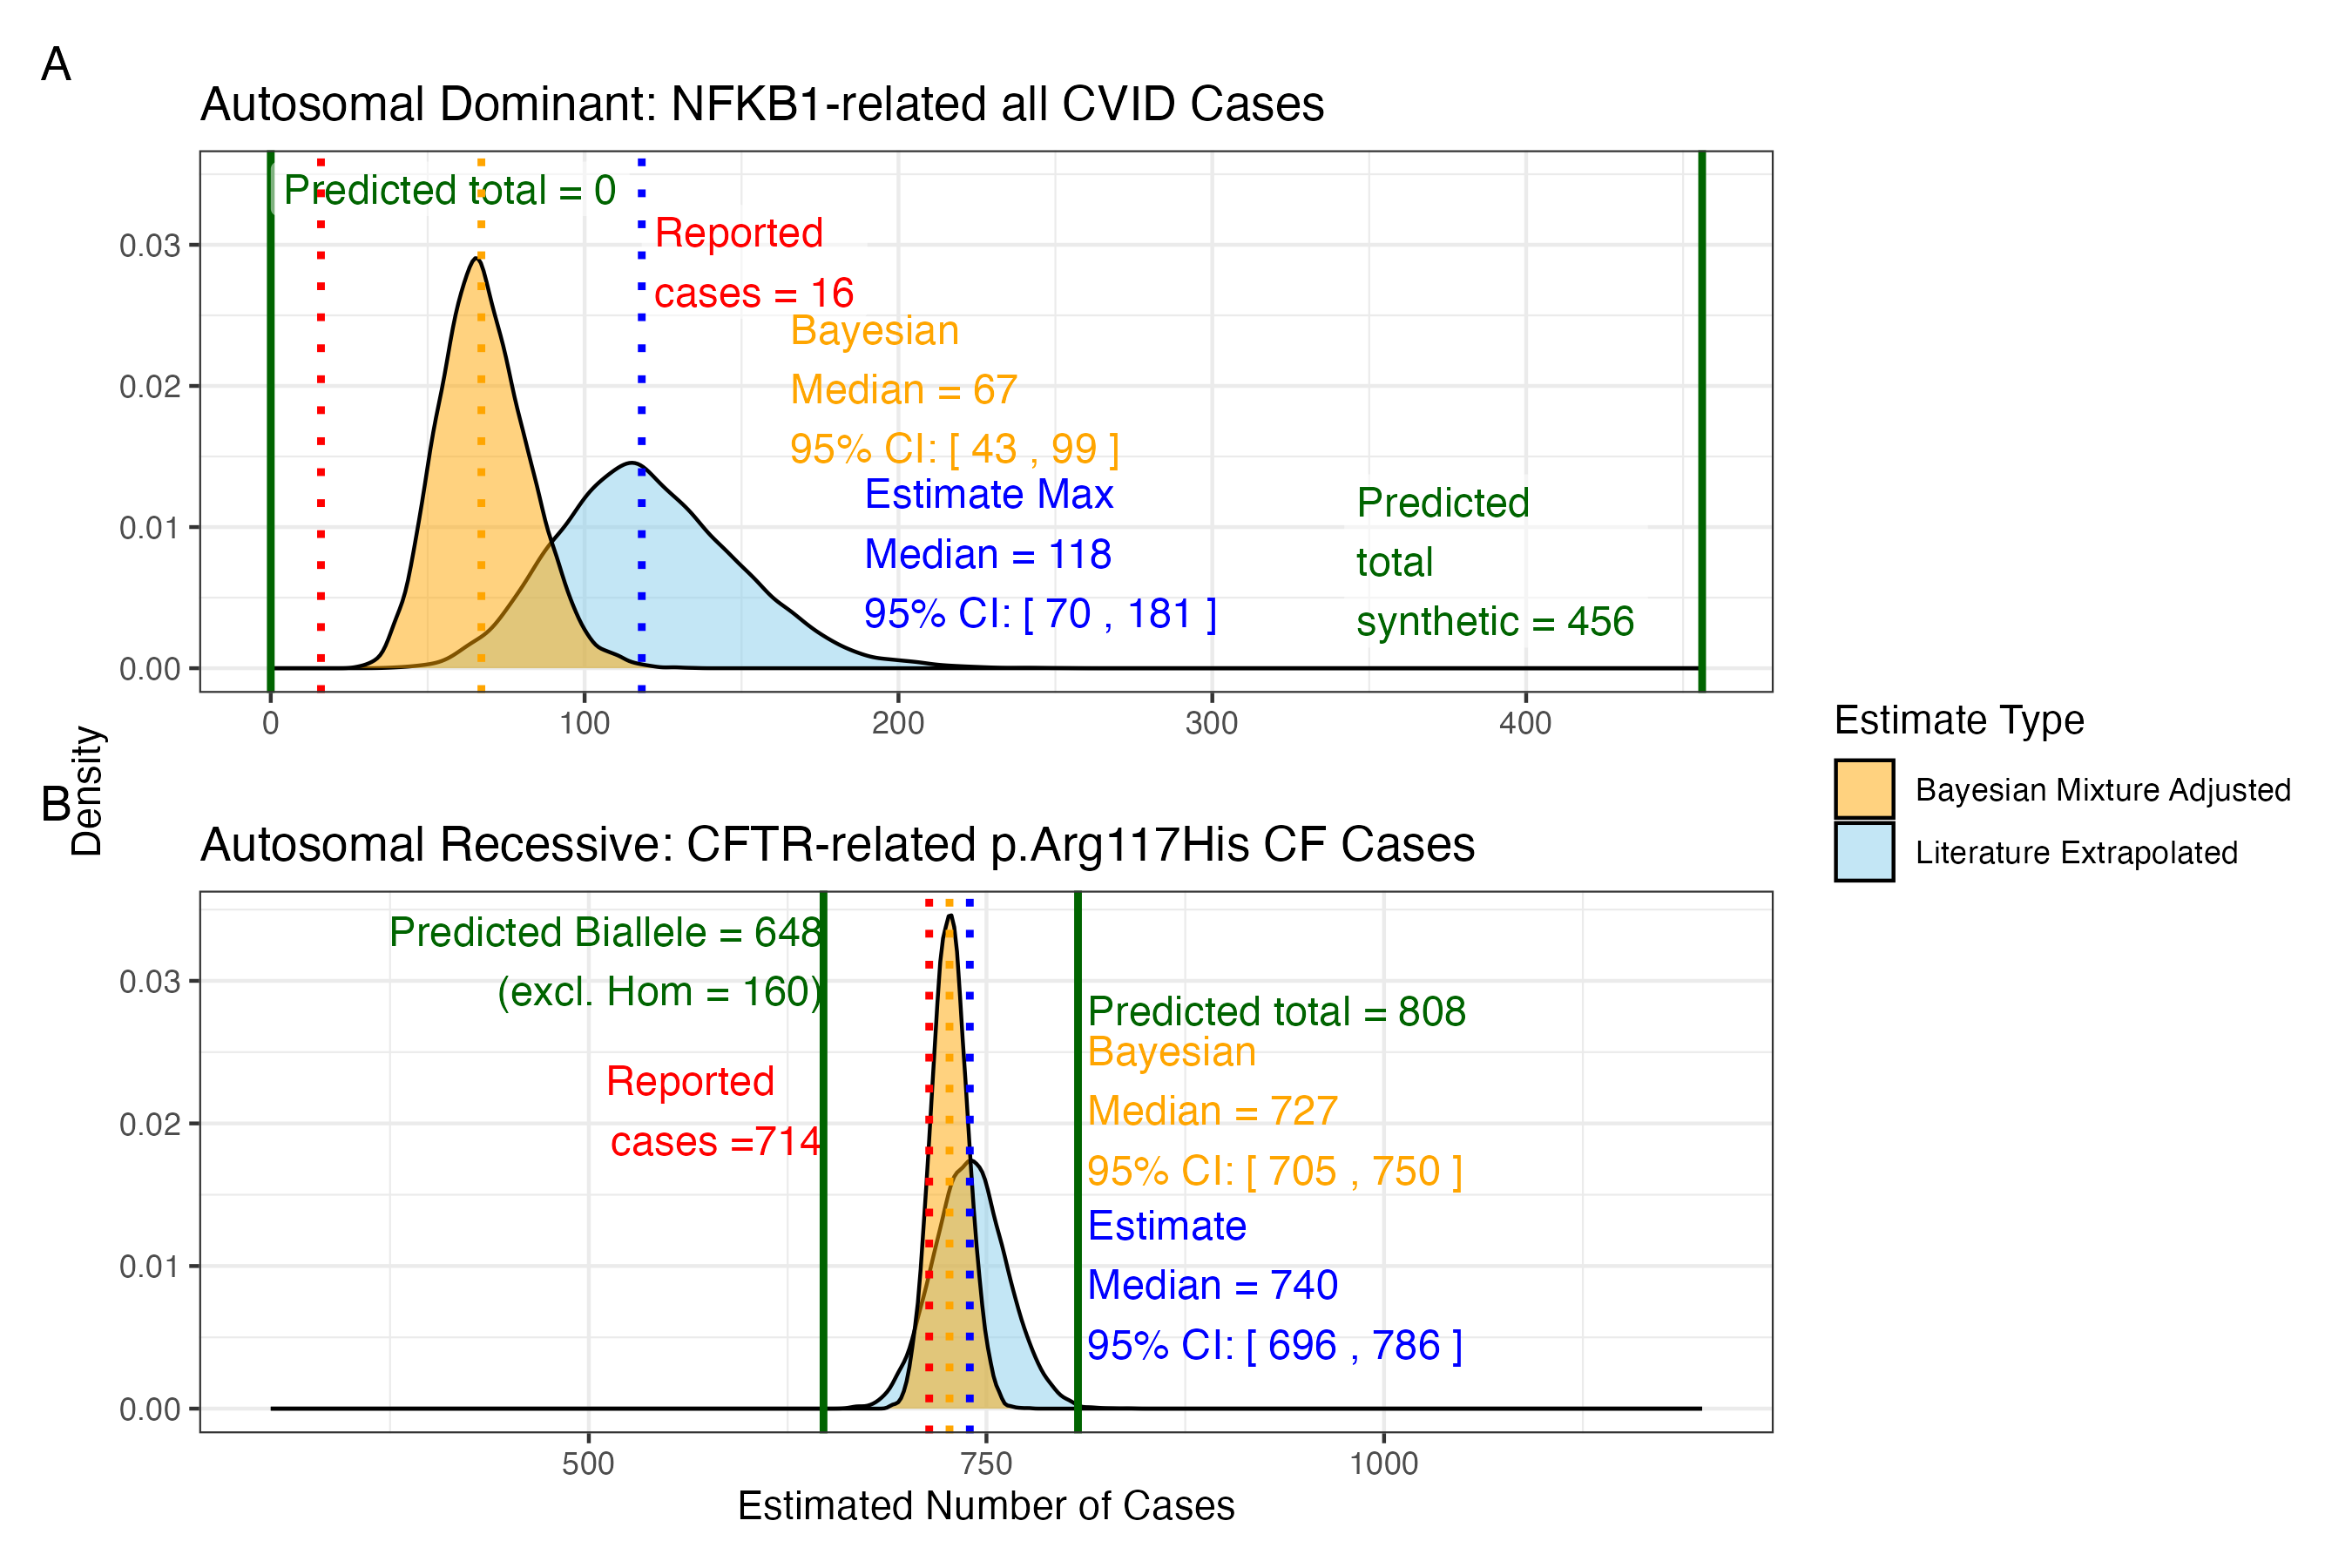
\includegraphics[width=0.99\textwidth]{../images/validation_studies_bayesian_adjusted_estimates.png}
  \caption{\textbf{Prior probabilities compared to validation disease cohort metrics.}
  (A) Density distributions for the number of \ac{nfkb1}-related \ac{cvid} cases in the UK. 
  Our model (green) predicted 456 cases, which falls between the observed cohort count (red) of 390 and the upper extrapolated values.
  The blue curve represents maximum count of 1280, and the orange curve shows the Bayesian-adjusted mixture estimate of 835. 
(B) Density distributions for \ac{cftr}-related p.Arg117His \ac{cf} cases. 
Our model (green) predicted 648 biallelic cases and 808 total cases.
The nationally reported case count (red) was 714.
The blue curve represents maximum extrapolated count of 740, and the orange curve shows the Bayesian-adjusted mixture estimate of 727. We observed close agreement among the reported disease cases and our integrated probability estimation framework.}
  \label{fig:validation_studies_bayesian_adjusted_estimates}
\end{figure}

\begin{figure}[ht]
  \centering
  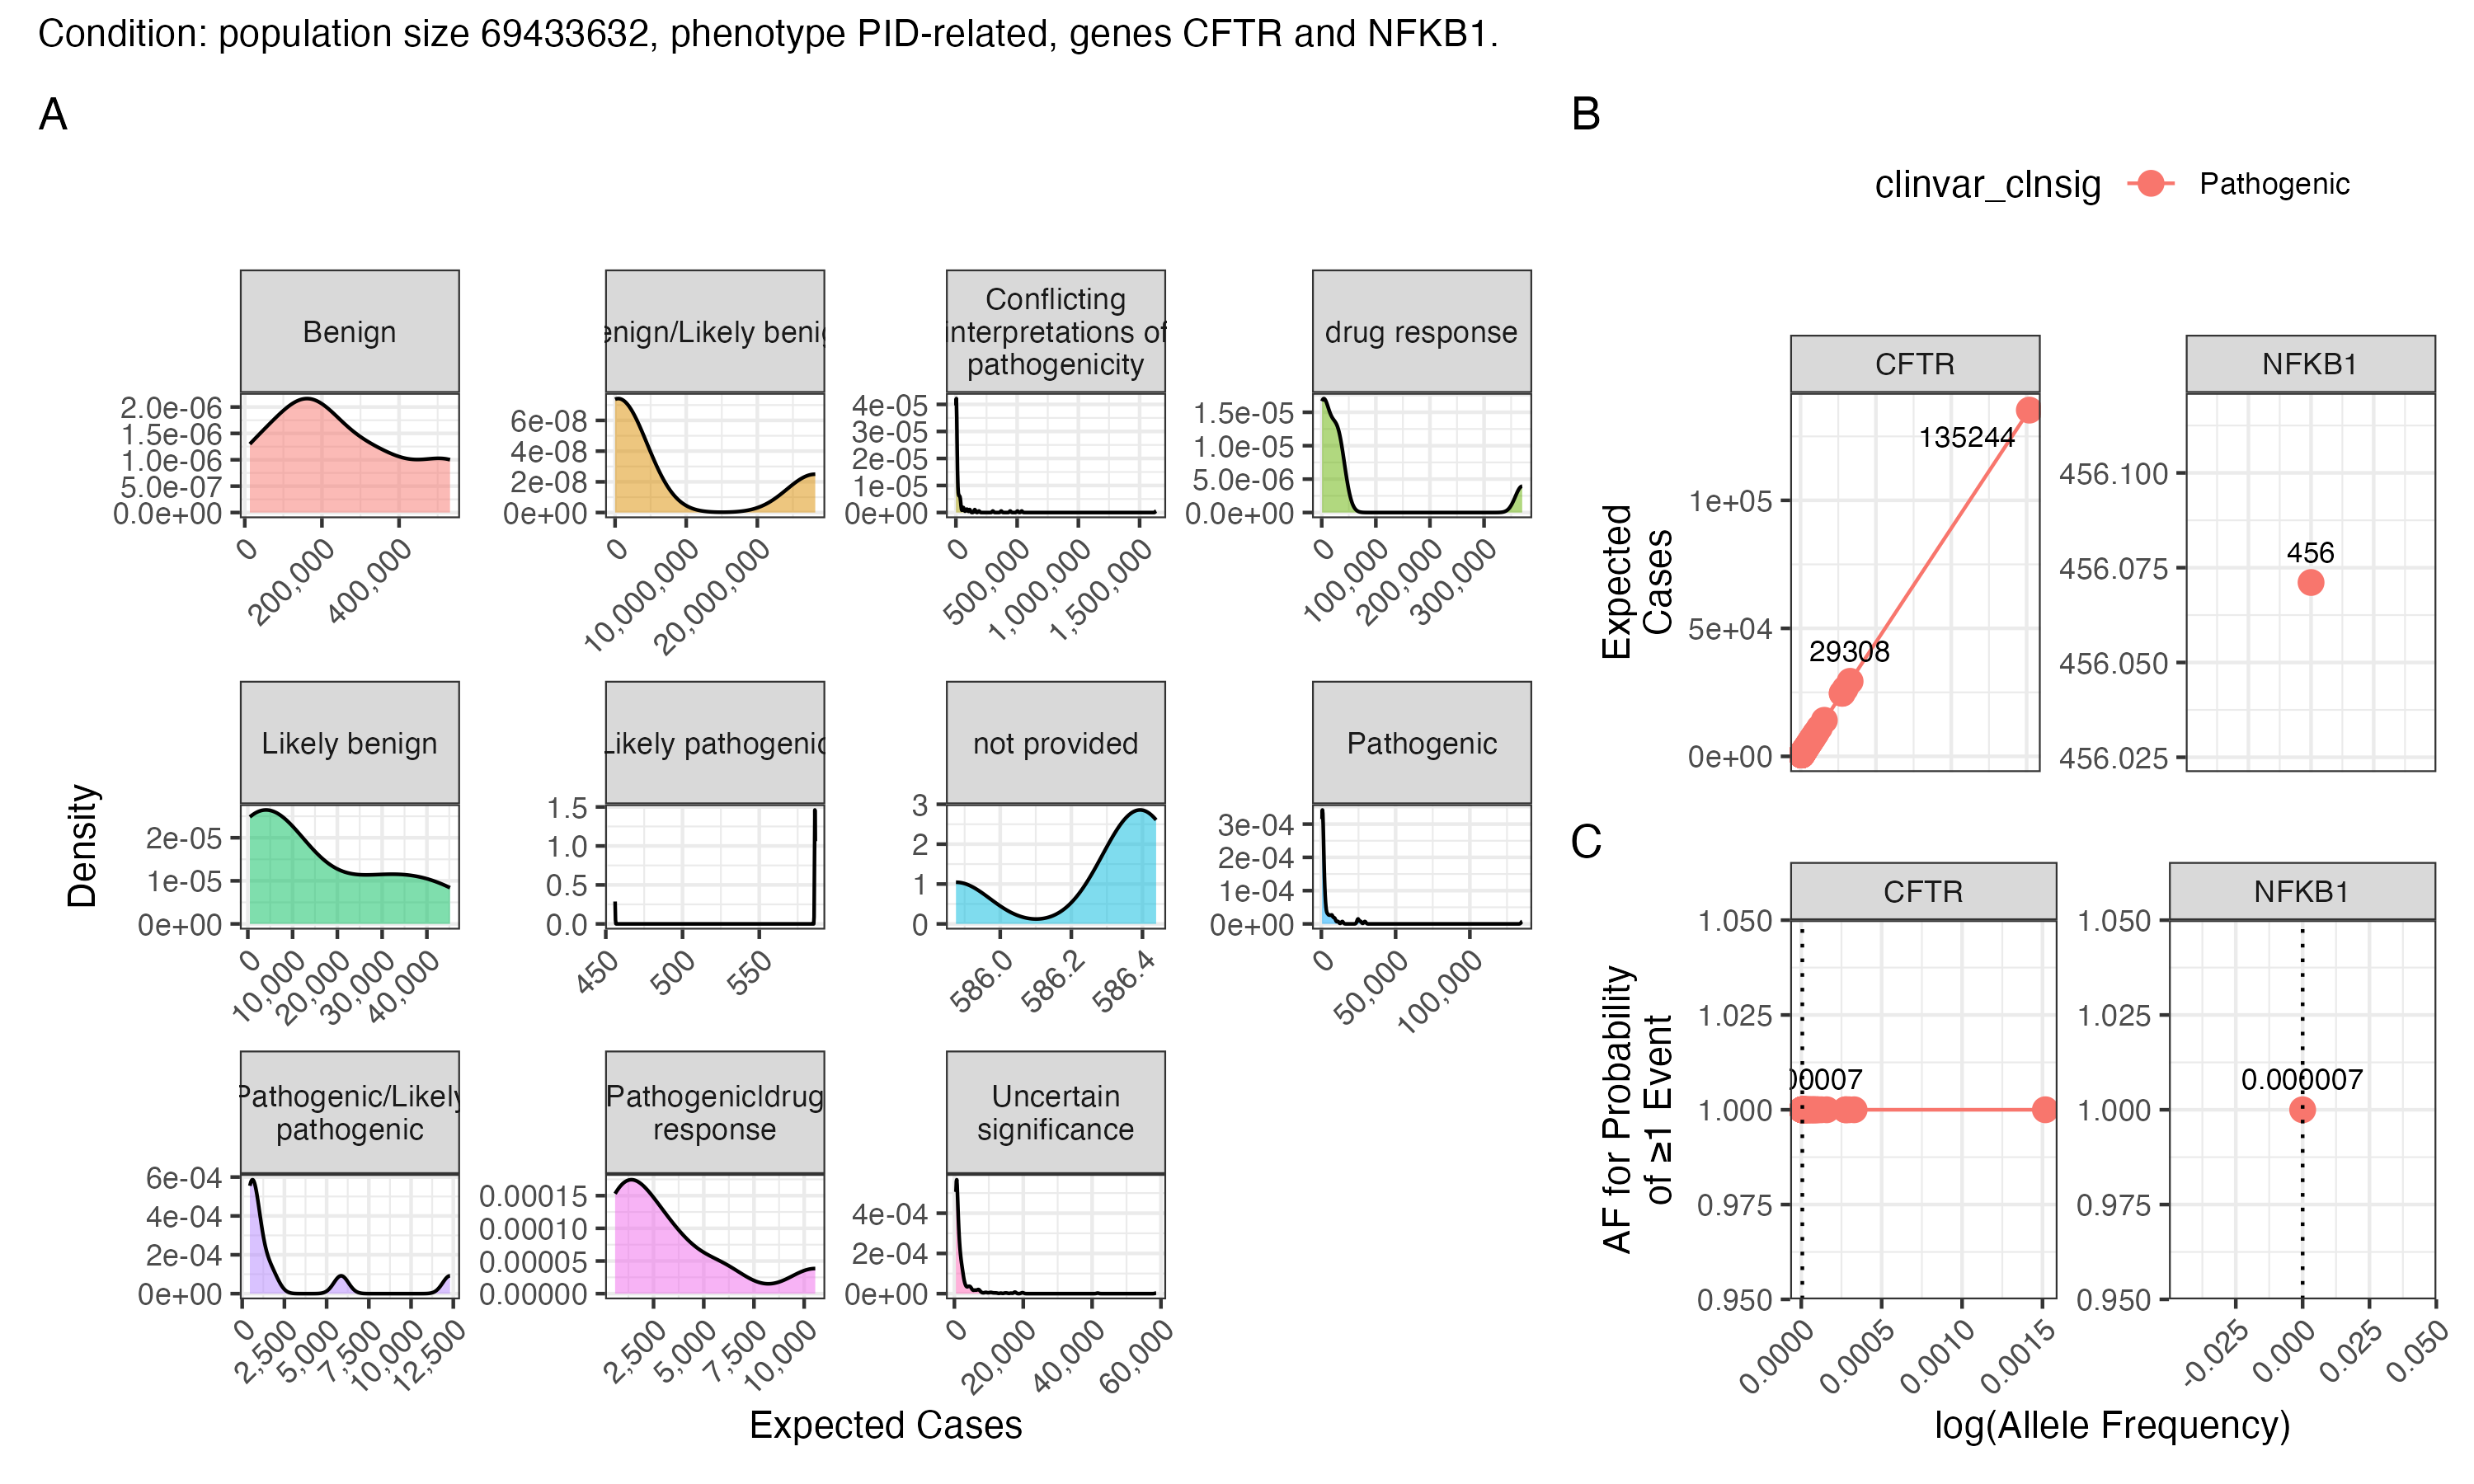
\includegraphics[width=\textwidth]{../images/validation_studies_scatterdense_expected_prob.png}
  \caption{\textbf{Interpretation of probability of observing a variant classification.} 
 The result from the chosen validation genes \ac{cftr} and \ac{nfkb1} are shown. 
 Case counts are dependant on the population size and phenotype.
(A) The density plots of expected observations by ClinVar clinical significance. 
We then highlight the values for pathogenic variants specifically showing;
(B) the allele frequency versus expected cases in this population size and
(C) the probability of observing at least one event in this population size.}
  \label{fig:validation_scatter_dense}
\end{figure}

\begin{figure}[ht]
  \centering
  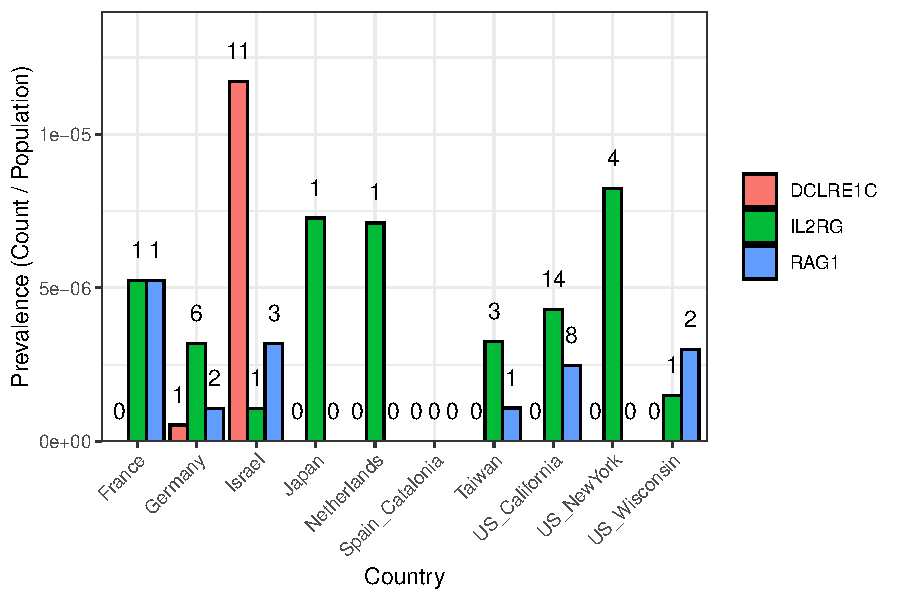
\includegraphics[width=.75\textwidth]{../images/validation_studies_scid_gene_comparison.pdf}
  \caption{\textbf{SCID-specific gene comparison across regions.} The bar plot shows the prevalence of SCID-related cases (count divided by population) for each gene and country (or region), with numbers printed above the bars representing the actual counts in the original cohort (ranging from 0 to 11 per region and gene).}
  \label{fig:scid_gene_comparison}
\end{figure}

\begin{figure}[ht]
  \centering
  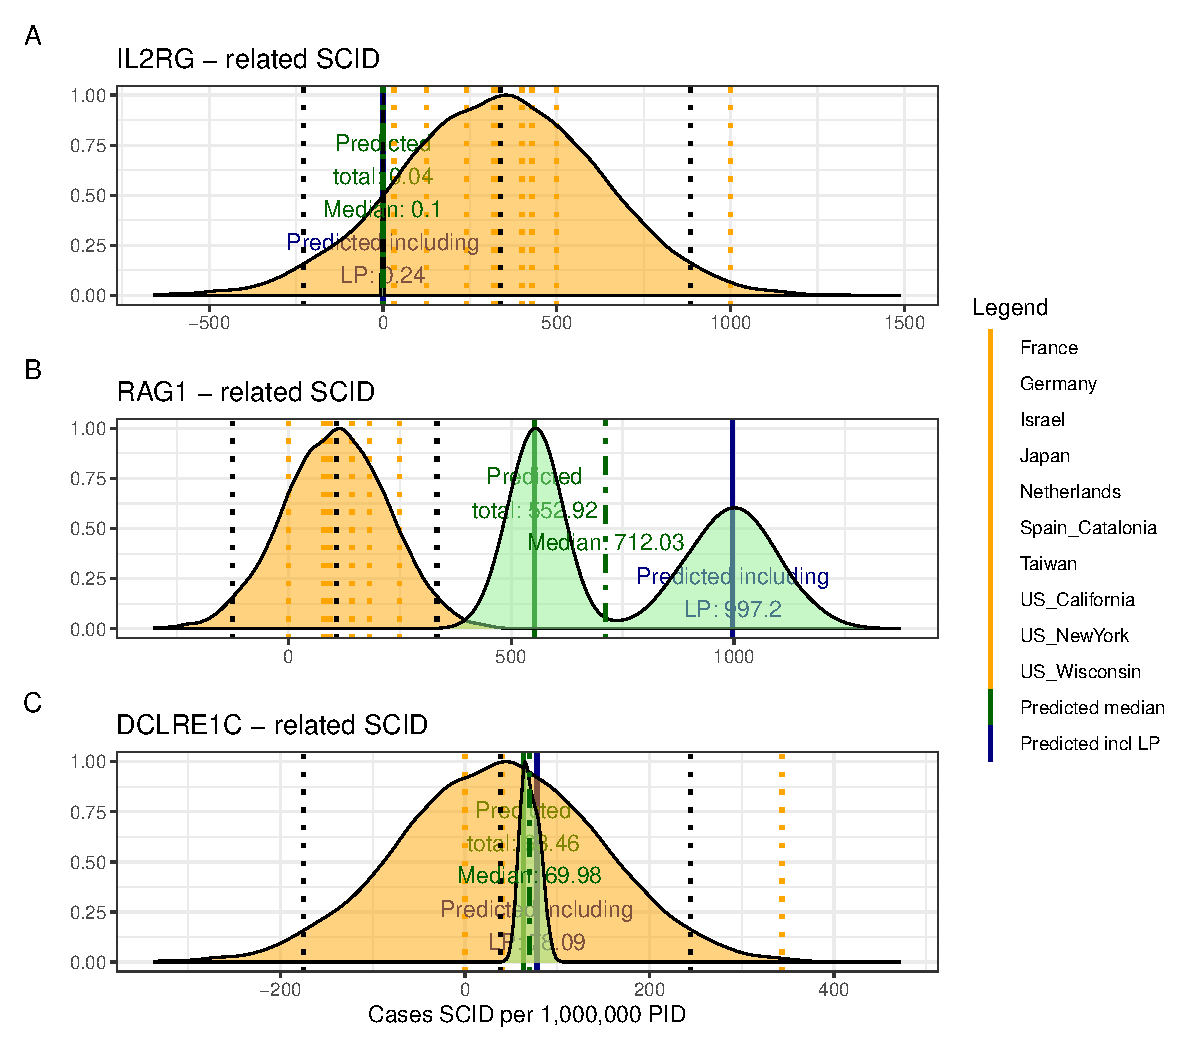
\includegraphics[width=.75\textwidth]{../images/validation_studies_scid_combined_plot.pdf}
  \caption{\textbf{Combined SCID-specific Predictions and Observed Rates per 1,000,000 PID.}
    The figure presents density distributions for the predicted SCID case counts (per 1,000,000 PID) for three genes: \textit{IL2RG}, \textit{RAG1}, and \textit{DCLRE1C}. Country-specific rates (displayed as dotted vertical lines) are overlaid with the overall predicted distributions for pathogenic and likely pathogenic variants (solid lines with annotated medians). For \textit{IL2RG}, the low predicted value is consistent with the high deleteriousness of loss-of-function variants in this X-linked gene, while \textit{RAG1} exhibits considerably higher predicted counts, reflecting its lower penetrance in an autosomal recessive context.}
  \label{fig:scid_combined}
\end{figure}



\FloatBarrier
\subsection{Hierarchical Clustering of Enrichment Scores for Major Disease Categories}
\begin{figure}[ht]
  \centering
  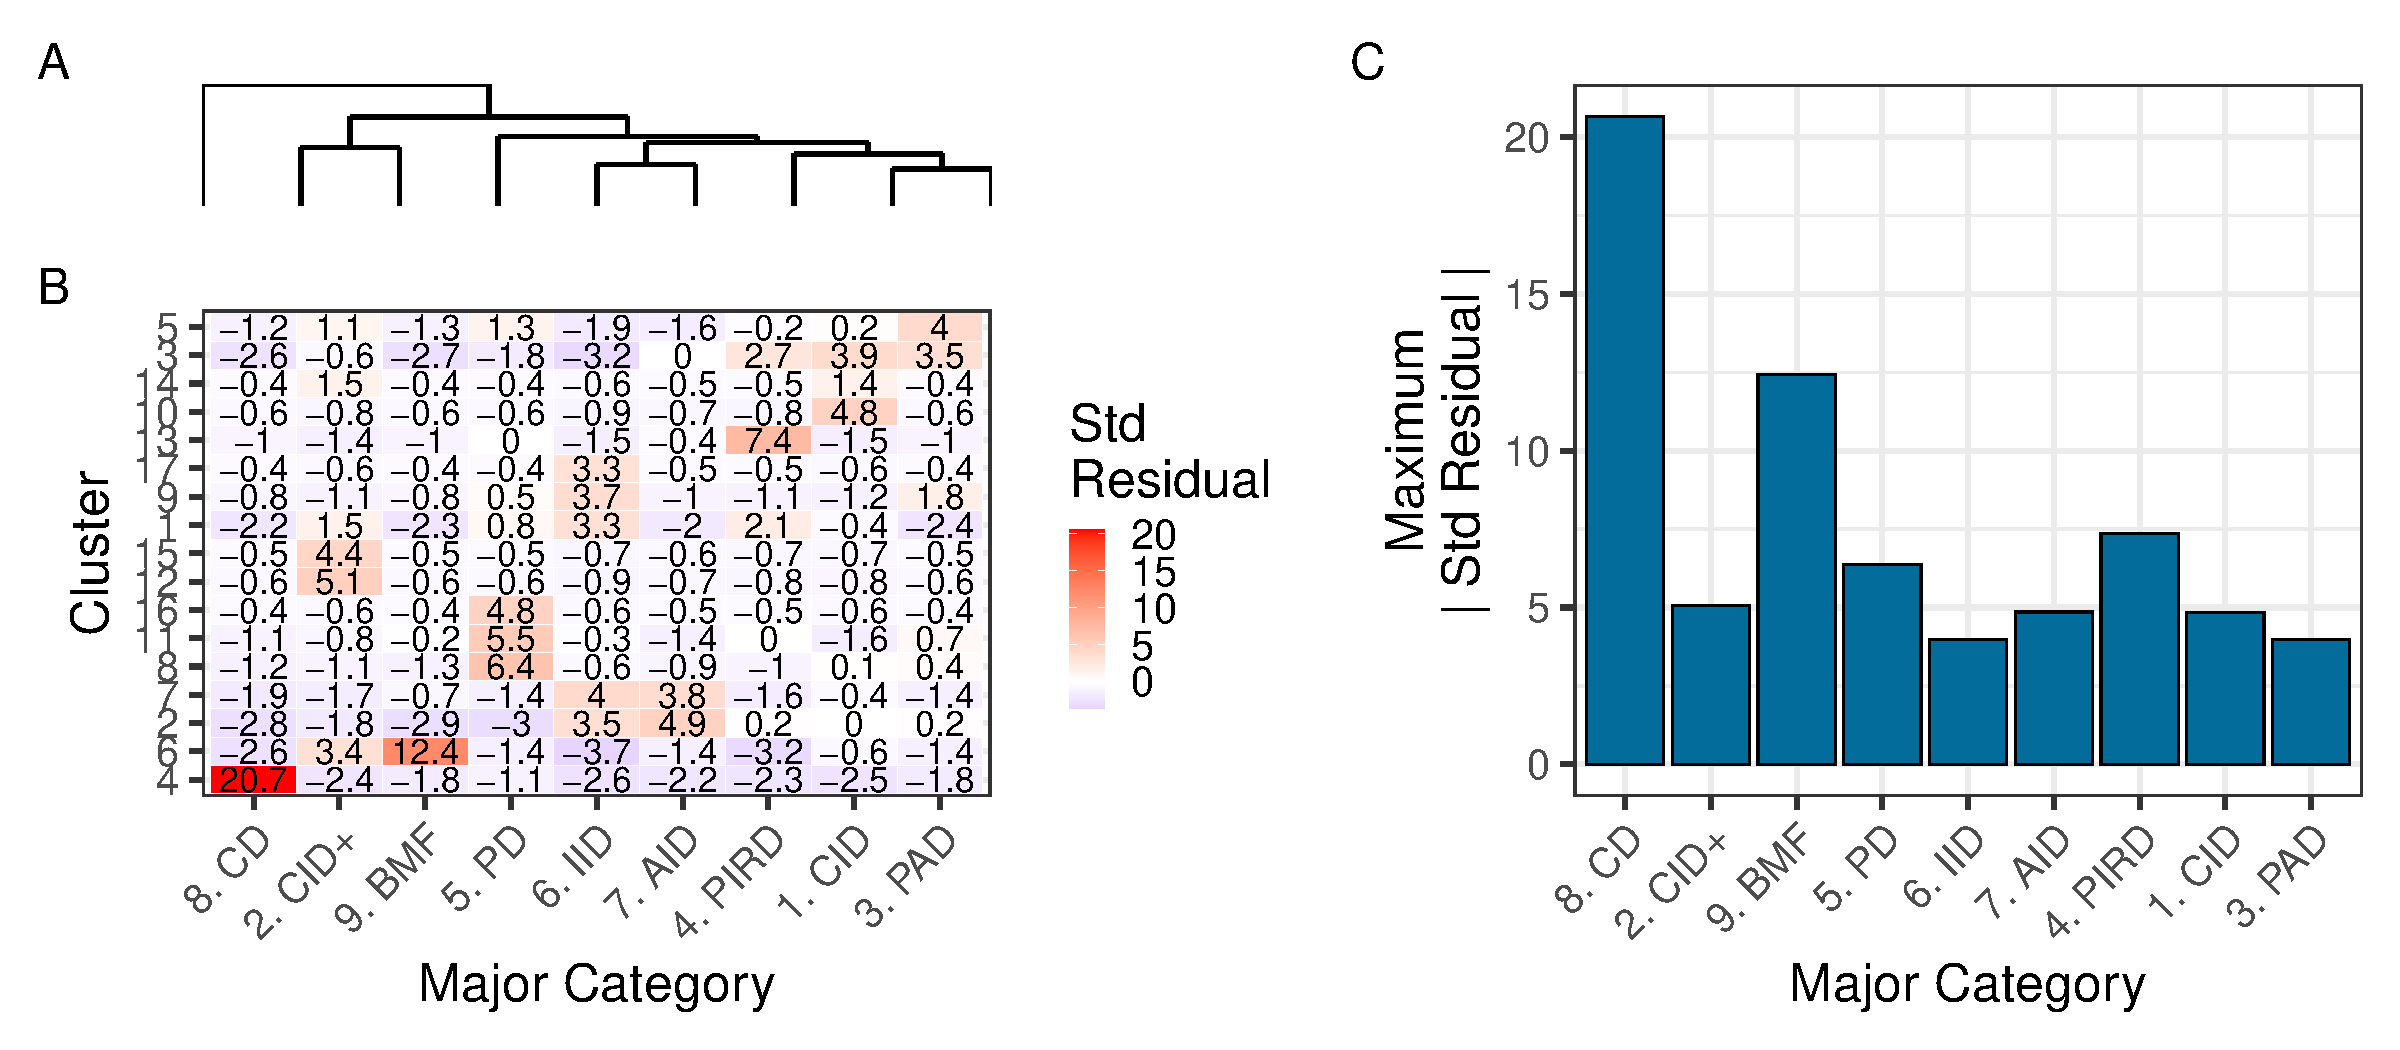
\includegraphics[width=0.99\textwidth]{../images/untangleR_ppi_network_patch2_cator.pdf}
  \caption{
   \textbf{Hierarchical clustering of enrichment scores.}
    The heatmap displays standardised residuals for major disease categories (x-axis) across network clusters (y-axis). A dendrogram groups similar disease categories, and the bar plot shows the maximum absolute residual per category.  (8) \ac{cd} and (9)\ac{bmf} show the highest vales, indicating significant enrichment or depletion (residuals > |2|). Definitions in \textbf{Box \ref{box:definitions}}.
  }
  \label{fig:patch2}
\end{figure}

\begin{figure}[ht]
  \centering
  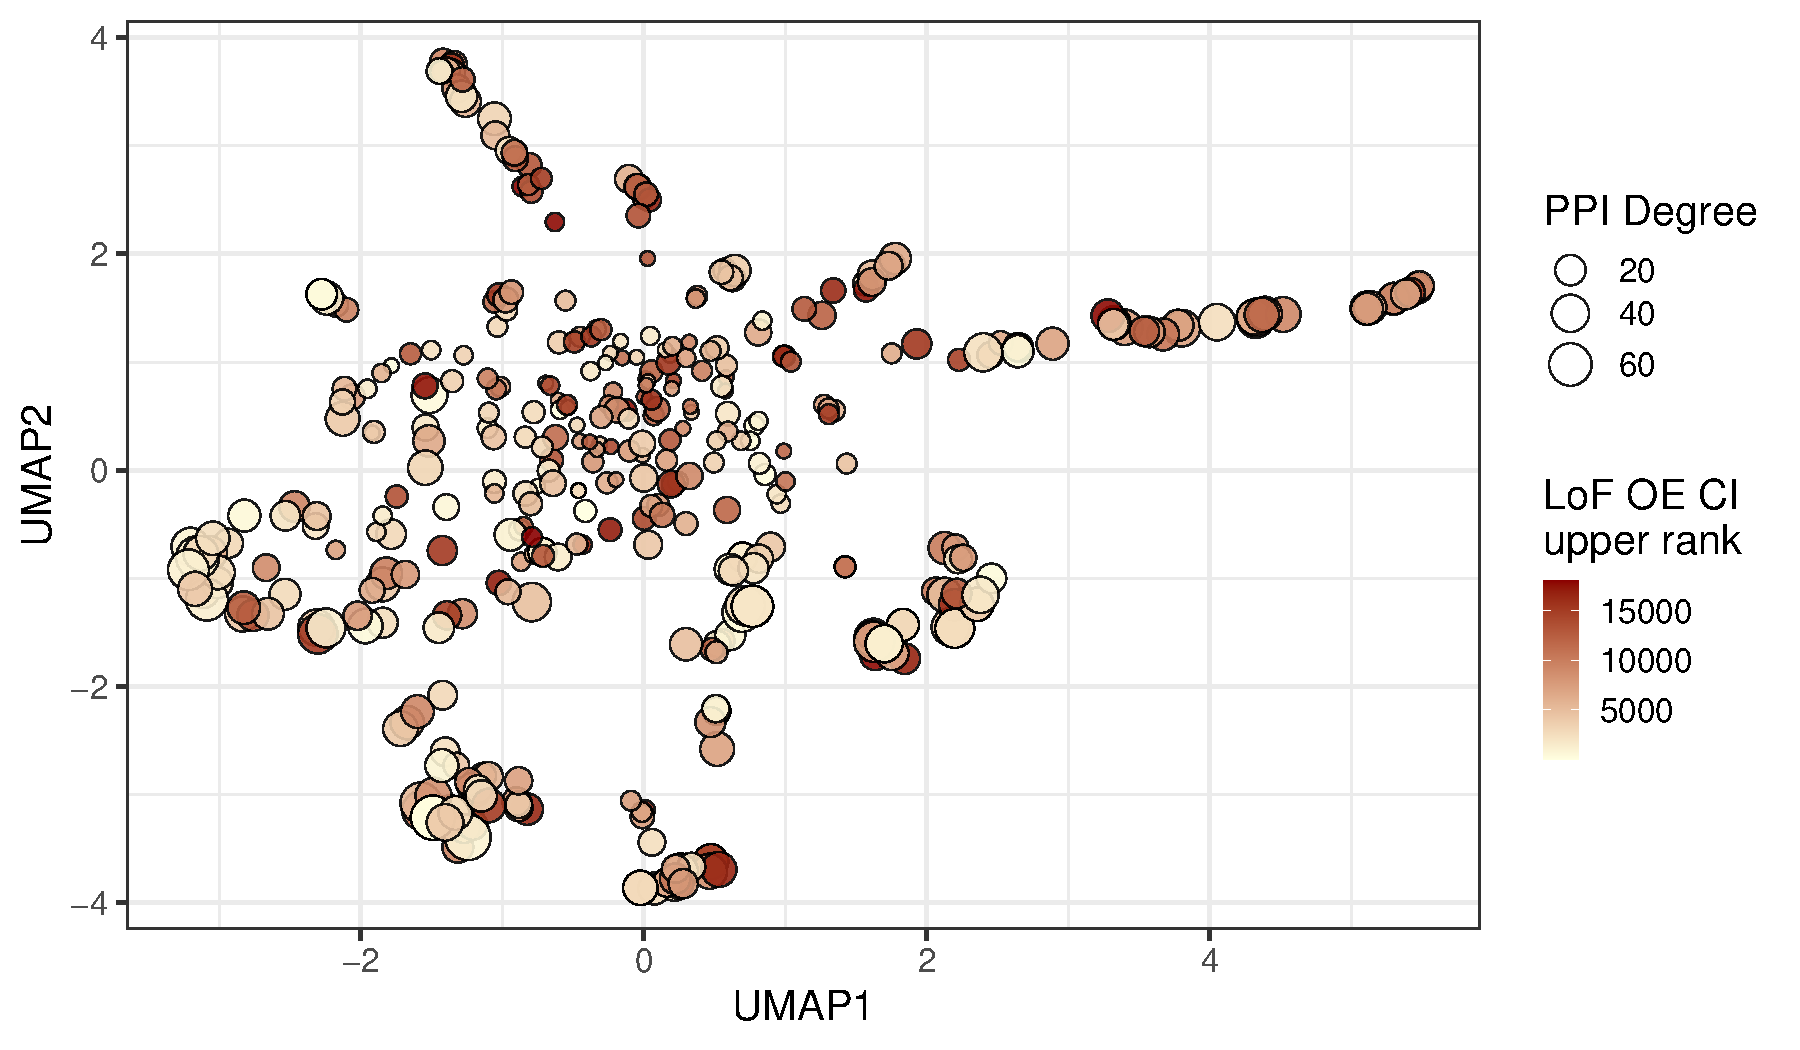
\includegraphics[width=0.99\textwidth]{../images/untangleR_ppi_network_p_umap_const.pdf}
  \caption{
   \textbf{Analysis of \ac{ppi} degree versus \ac{loeuf} upper rank with \ac{umap} embedding of the \ac{ppi} network.}
    The relationship between \ac{ppi} degree (size) and \ac{loeuf} upper rank (color) across gene clusters. No clear patterns are evident.
  }
  \label{fig:p_umap_const}
\end{figure}

\begin{figure}[ht]
\centering
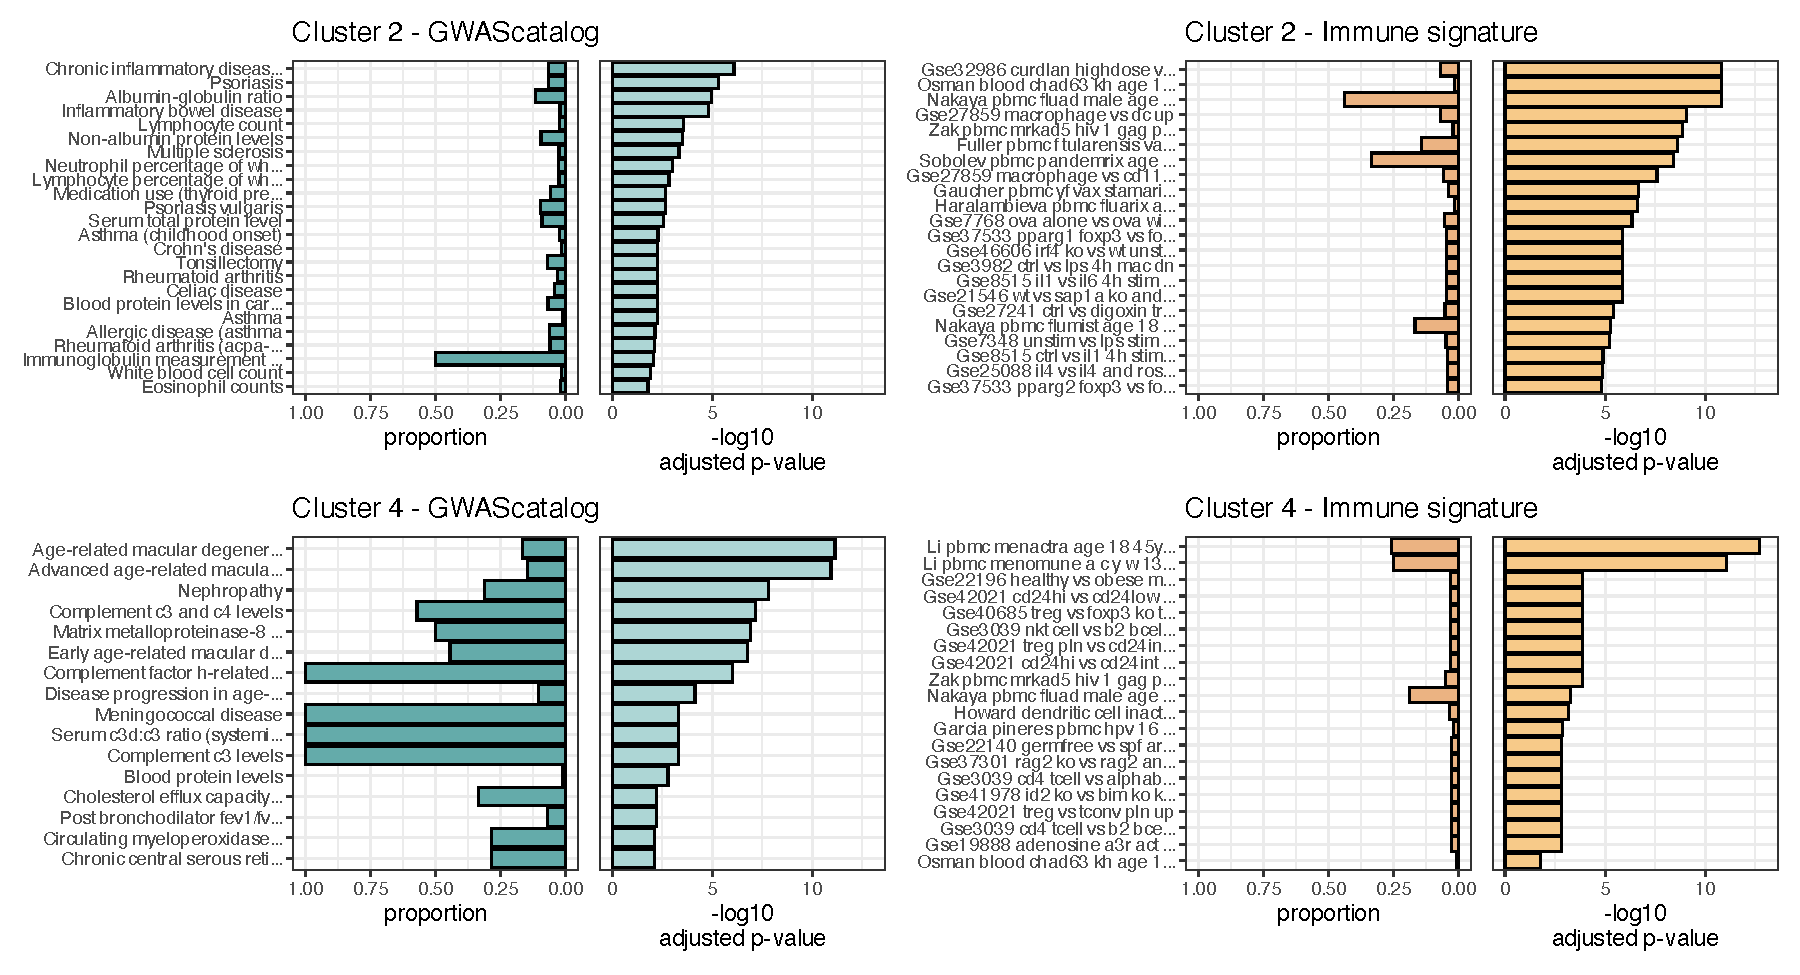
\includegraphics[width=0.99\textwidth]{../images/fuma_merge.pdf}
\caption{\textbf{Composite Enrichment Profiles for \ac{iei} Gene Sets.} 
We selected the top two enriched clusters (as per \textbf{Figure \ref{fig:p_cor_spear_rho_sig_clust_patch3}}) and performed functional enrichment analysis derived from known disease associations. For each gene set, the left panel displays the proportion of input genes overlapping with a curated gene set, and the right panel shows the \(-\log_{10}\) adjusted p-value from hypergeometric testing. These profiles, stratified by cluster (Cluster 2 and Cluster 4) and by gene set category (GWAScatalog and Immunologic Signatures), highlight distinct enrichment patterns that reflect differential pathogenic variant loads in the \ac{iei} gene panels.}
\label{fig:fuma_merge}
\end{figure}

\begin{figure}[ht]
\centering
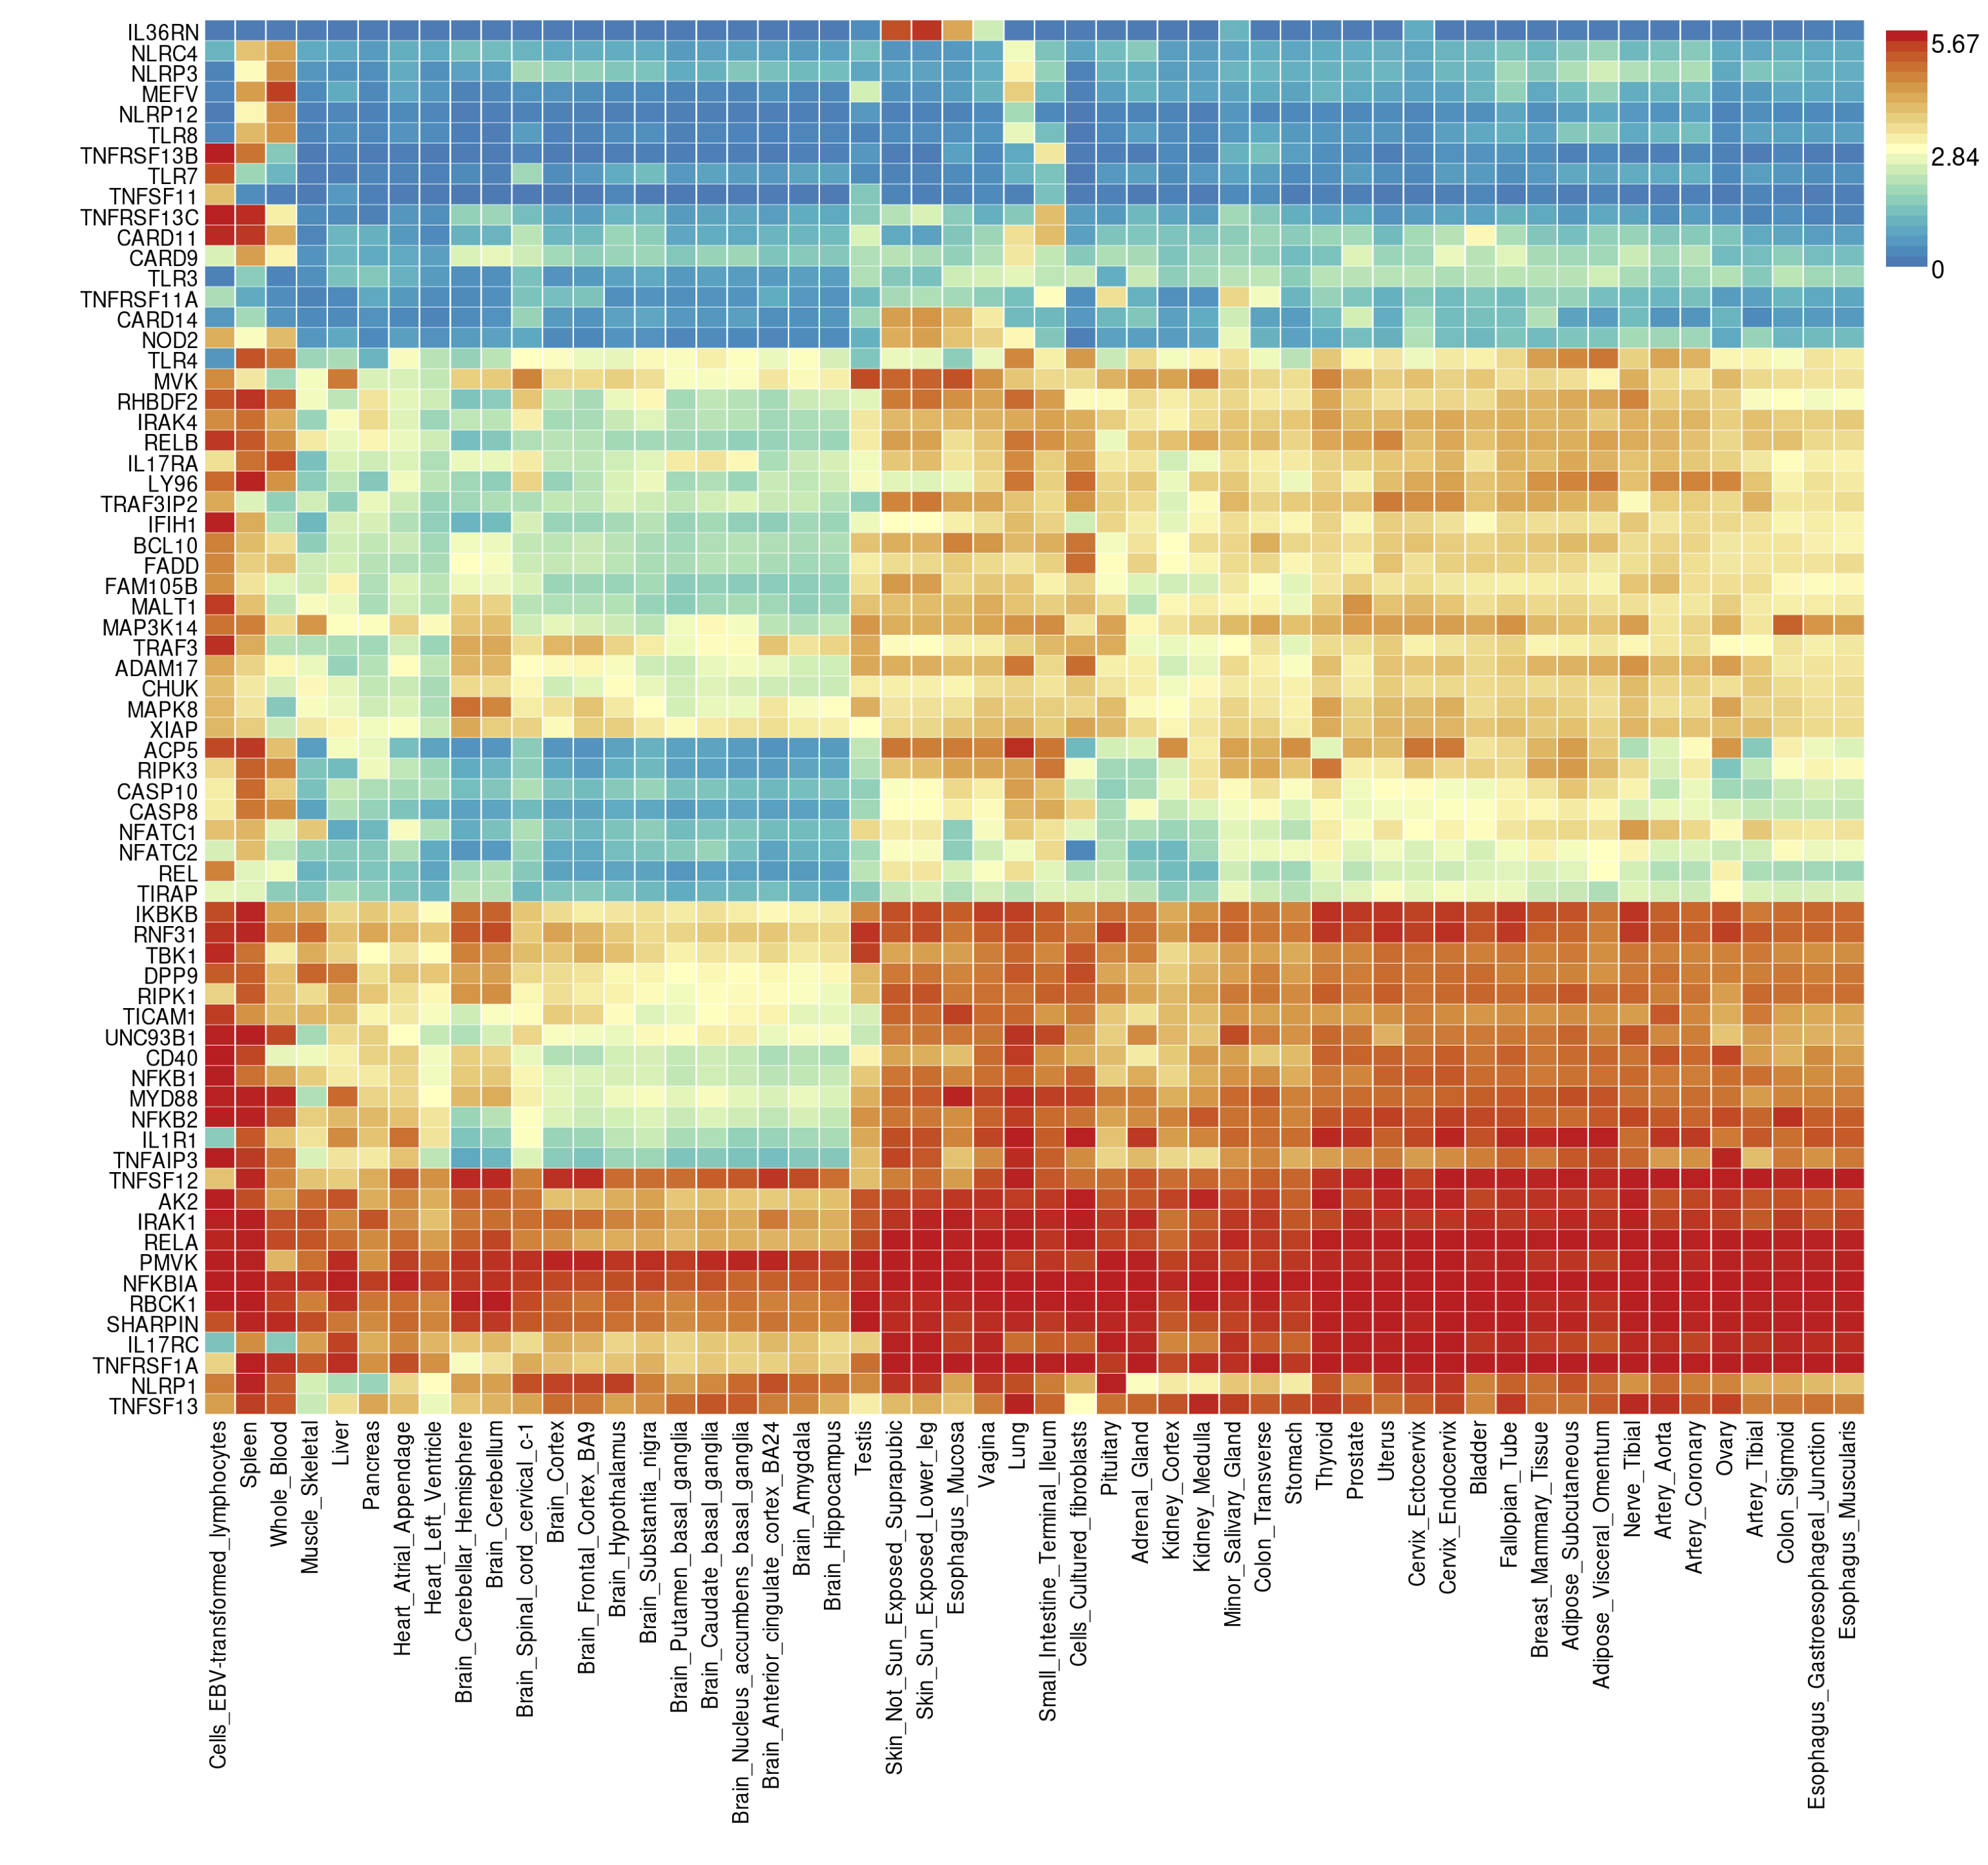
\includegraphics[width=0.75\textwidth]{../images/expHeat_FUMA_jobs604419_var_risk_est_cluster_2.png}
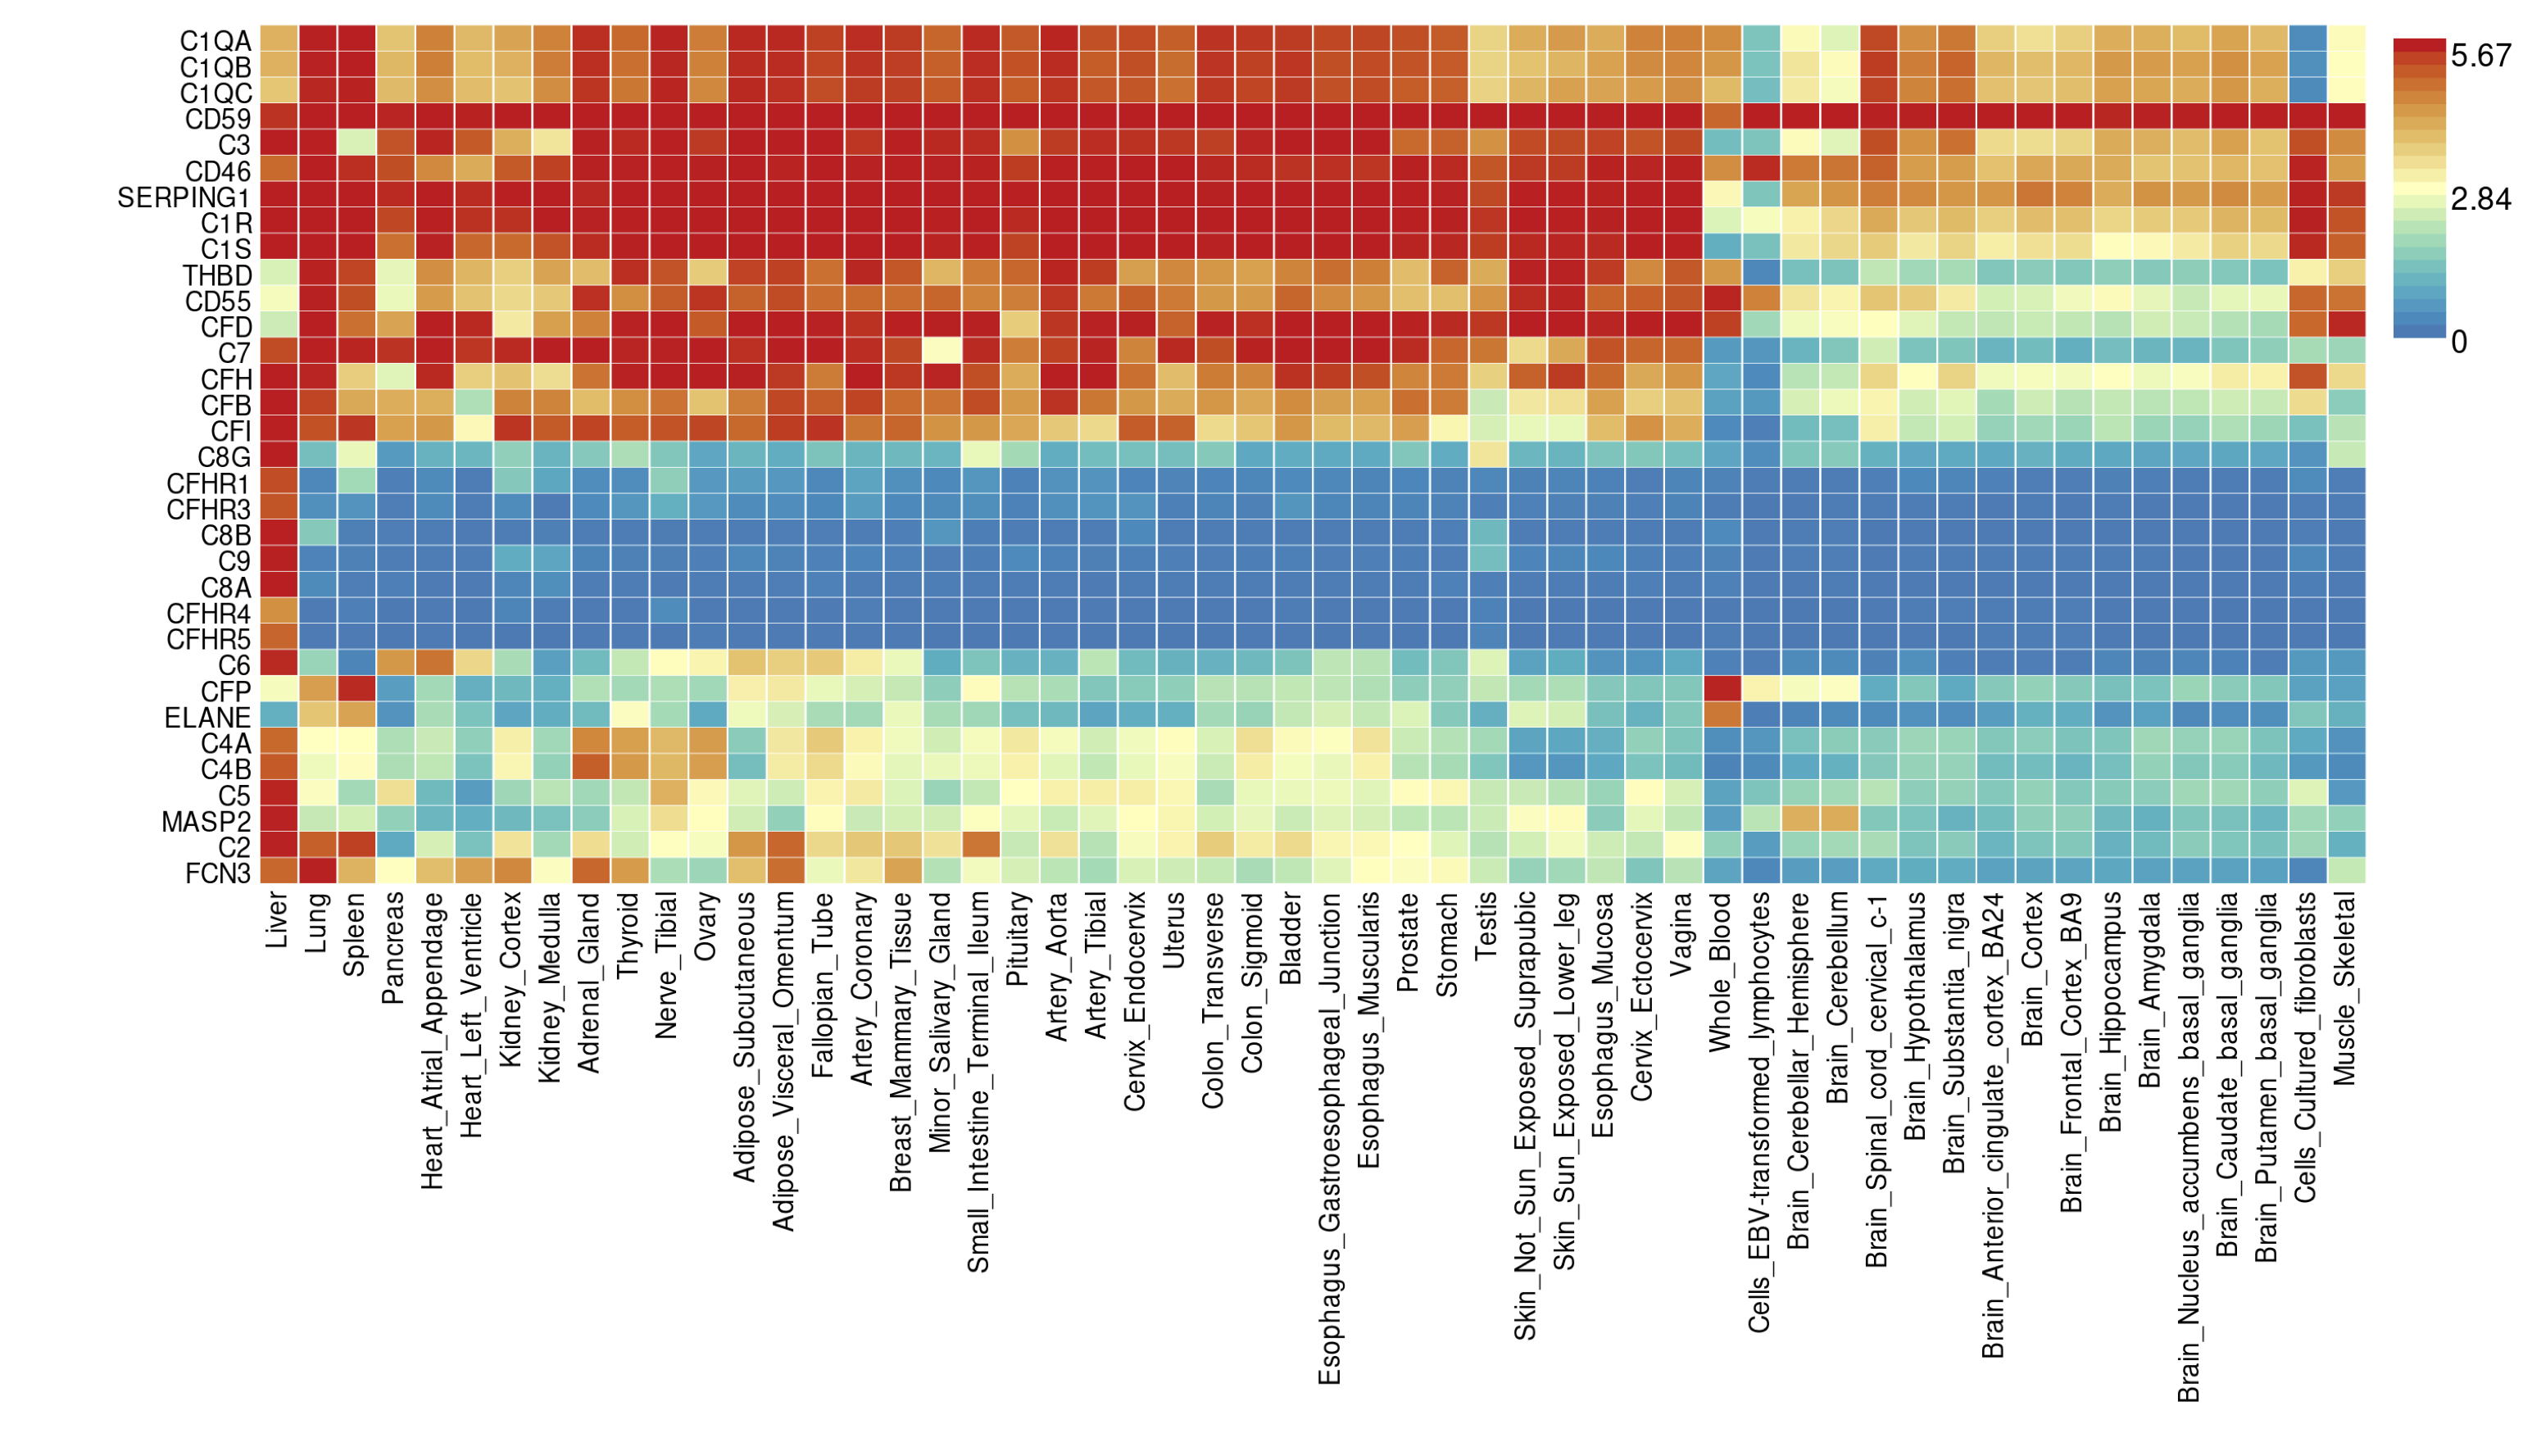
\includegraphics[width=0.75\textwidth]{../images/expHeat_FUMA_jobs604403_var_risk_est_cluster_4.png}
\caption{\textbf{Gene Expression Heatmaps for IEI Genes.} GTEx v8 data from 54 tissue types display the average expression per tissue label (log\(_2\) transformed) for the IEI gene panels. Top: Cluster 2; Bottom: Cluster 4.}
\label{fig:expHeatmaps}
\end{figure}

\FloatBarrier
\subsection{Interpretation of ClinVar Variant Observations}

\begin{figure}[ht]
  \centering
  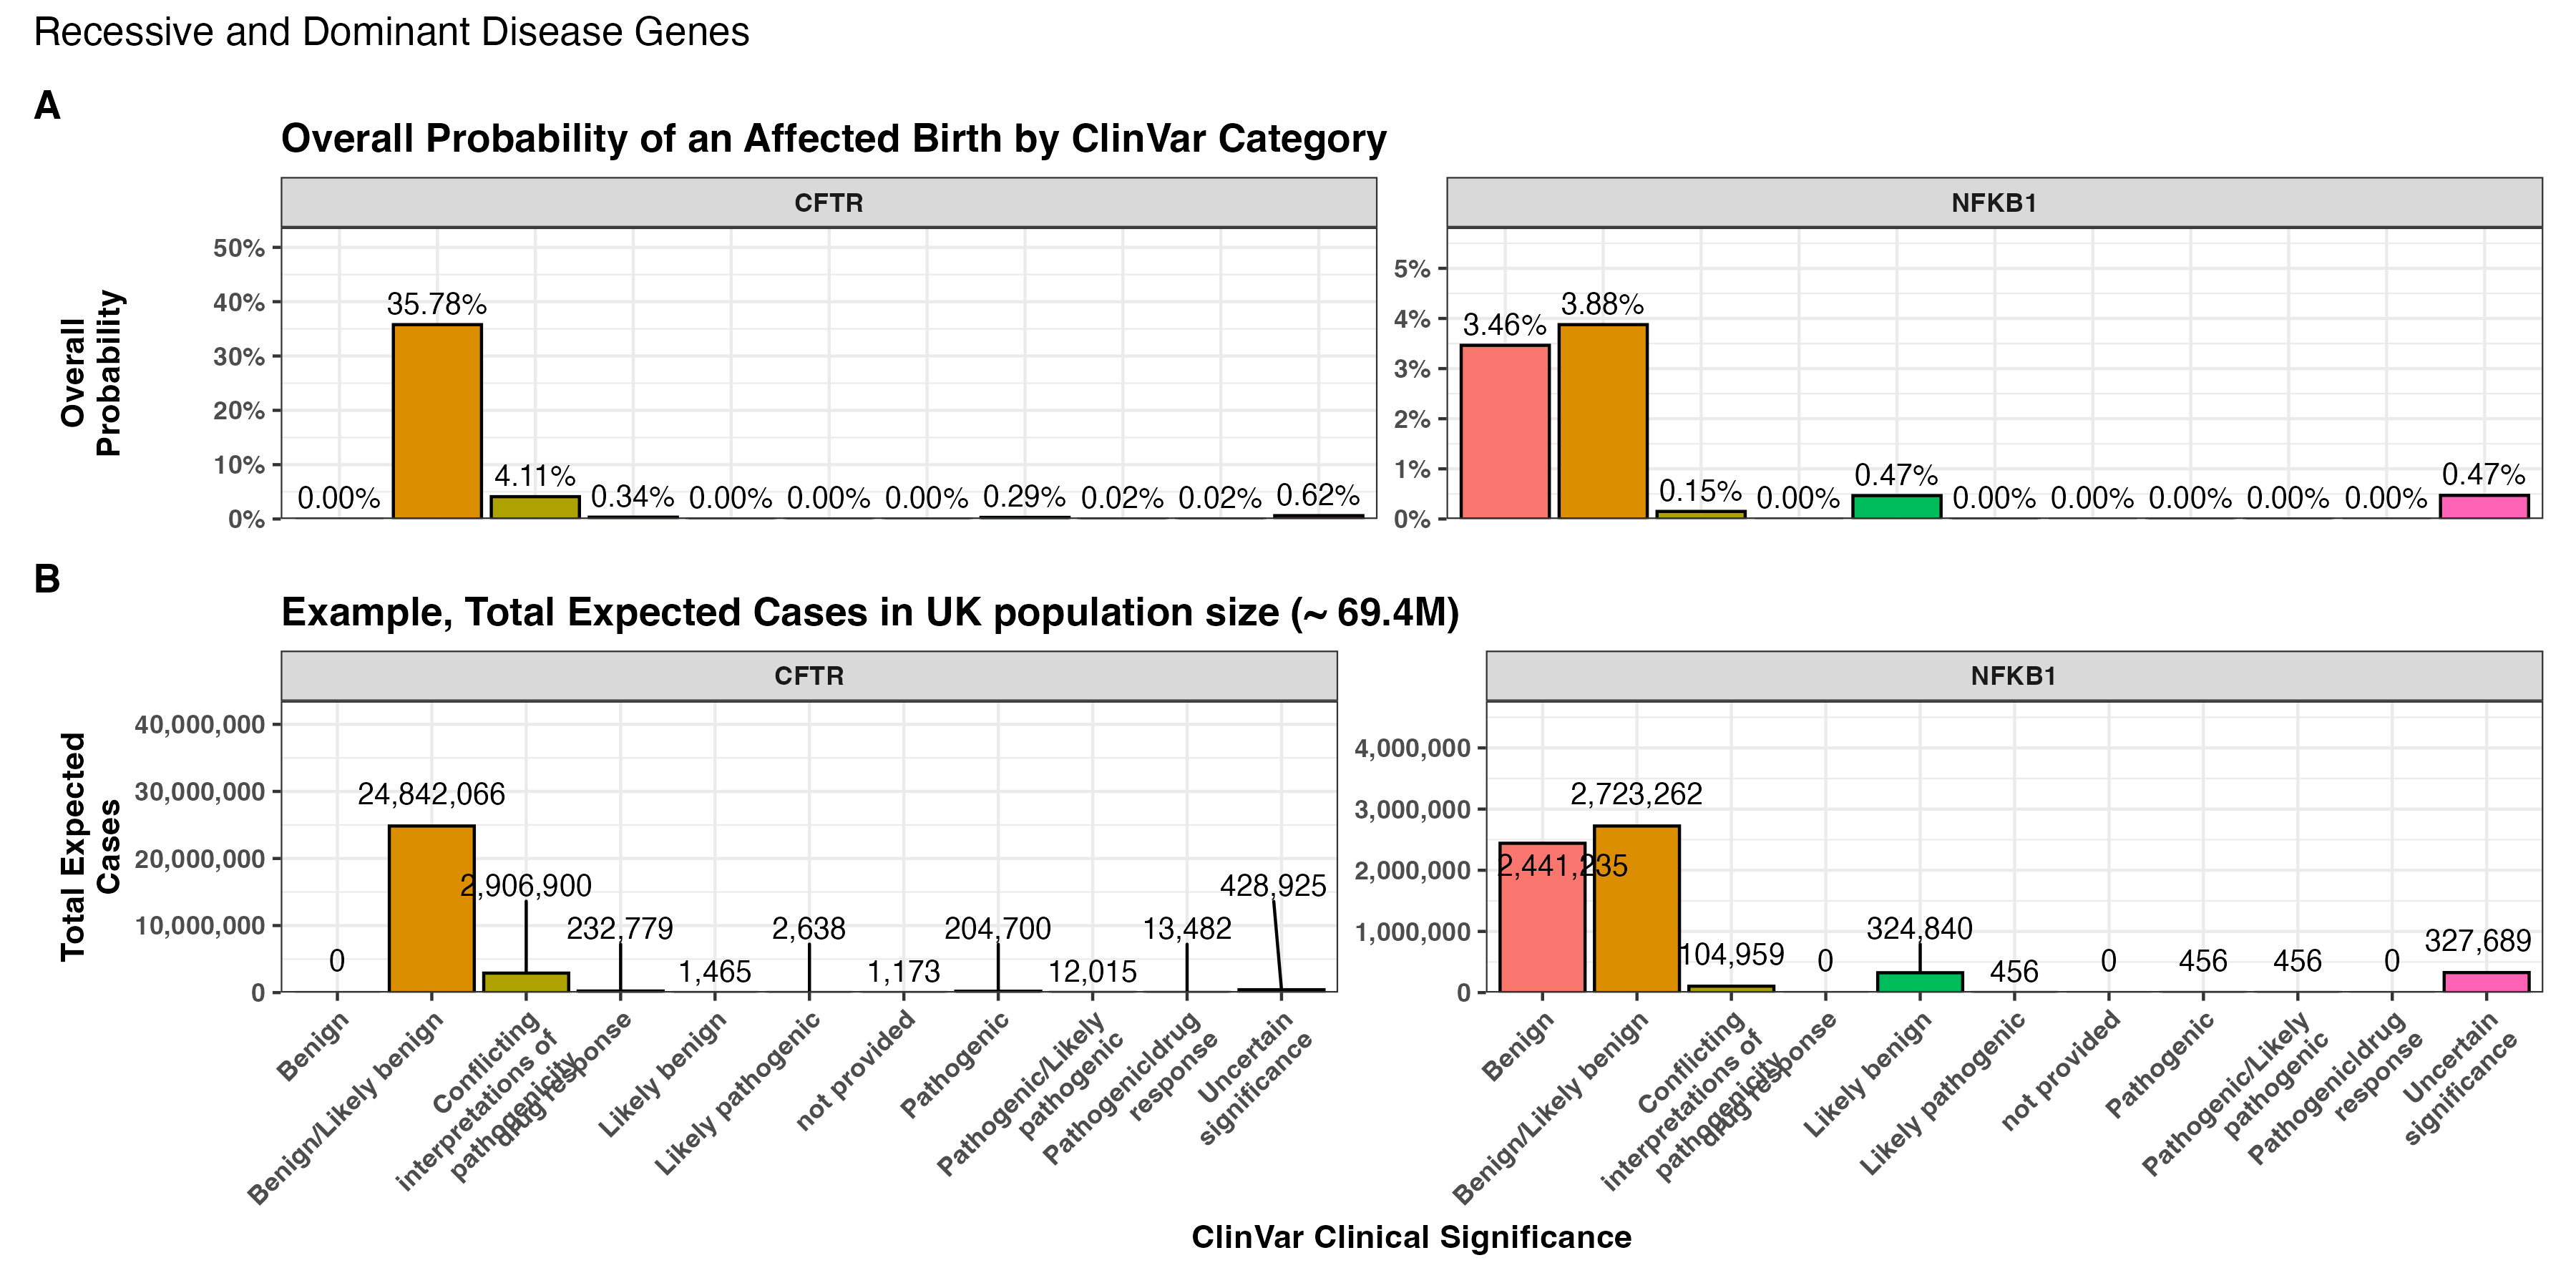
\includegraphics[width=0.99\textwidth]{../images/all_genes_combined_bar_charts_mini.png}
  \caption{\textbf{Combined bar charts summarizing the genome-wide analysis of ClinVar clinical significance for the \ac{pid} gene panel}. Panel (A) shows the overall probability of an affected birth by variant classification, and (B) displays the total expected number of cases per classification, both stratified by gene. These integrated results illustrate the variability in variant observations across genes and underpin our validation of the probability estimation framework.}
  \label{fig:all_genes_combined_bar_charts_mini}
\end{figure}


\FloatBarrier
\subsection{Novel PID classifications}



\begin{figure}[ht]
  \centering
  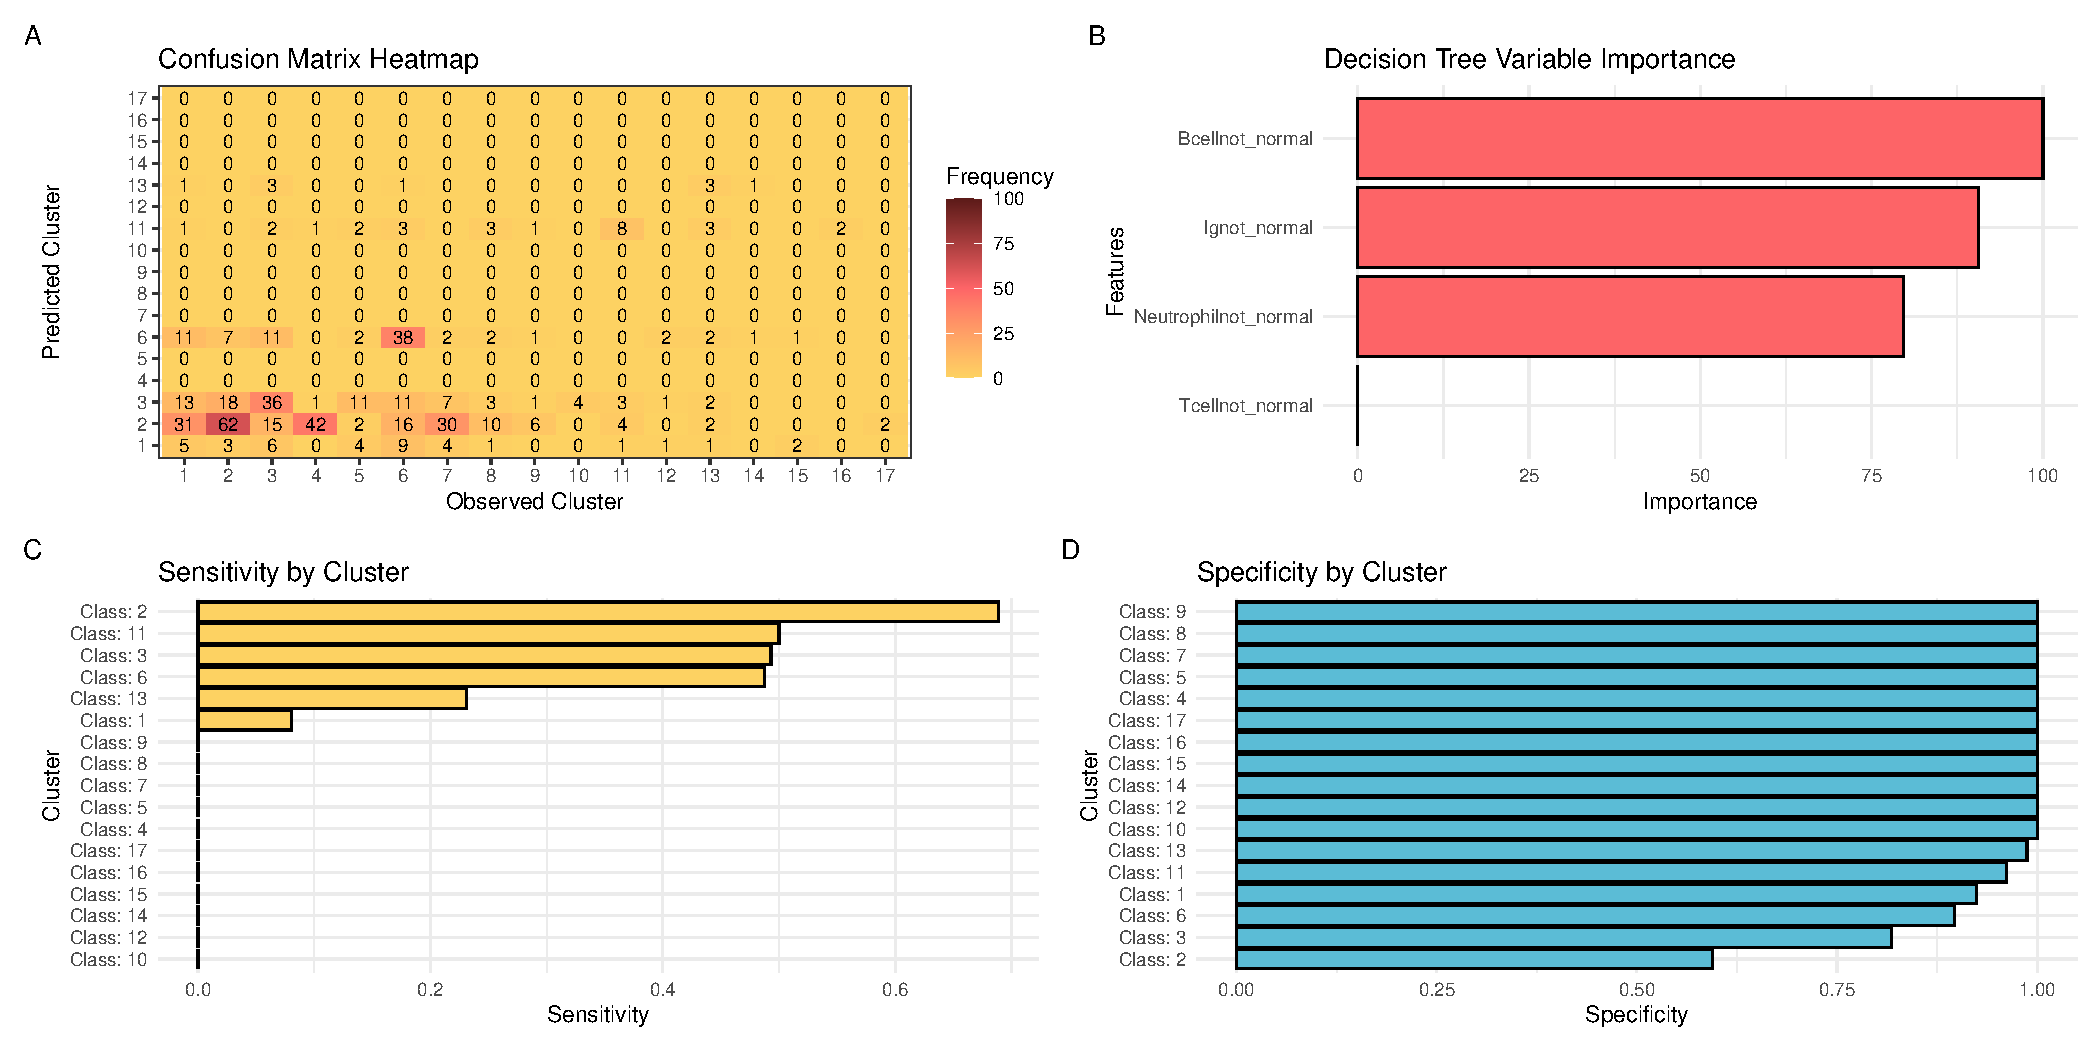
\includegraphics[width=0.99\textwidth]{../images/plot_combined_model_interpret_fine.pdf}
  % \caption{Model performance for fine-tuned PID classification. (A) Confusion matrix heatmap of observed versus predicted clusters. (B) Variable importance plot, and (C) per-class sensitivity and specificity bar plots derived from the decision tree model.}
  \caption{\textbf{Model performance for fine-tuned \ac{pid} classification.} (A) Confusion matrix heatmap comparing observed and predicted \ac{ppi} clusters. (B) Variable importance plot ranking immunophenotypic features contributing to the classifier. (C) Per-class sensitivity and (D) per-class specificity bar plots. These panels collectively demonstrate the performance of the decision tree classifier in stratifying \ac{pid} genes based on immunophenotypic and \ac{ppi} features.}
  
  \label{fig:confusion_matrix}
\end{figure}

\FloatBarrier
\subsection{Probability of observing AlphaMissense pathogenicity}

\begin{figure}[ht]
  \centering
  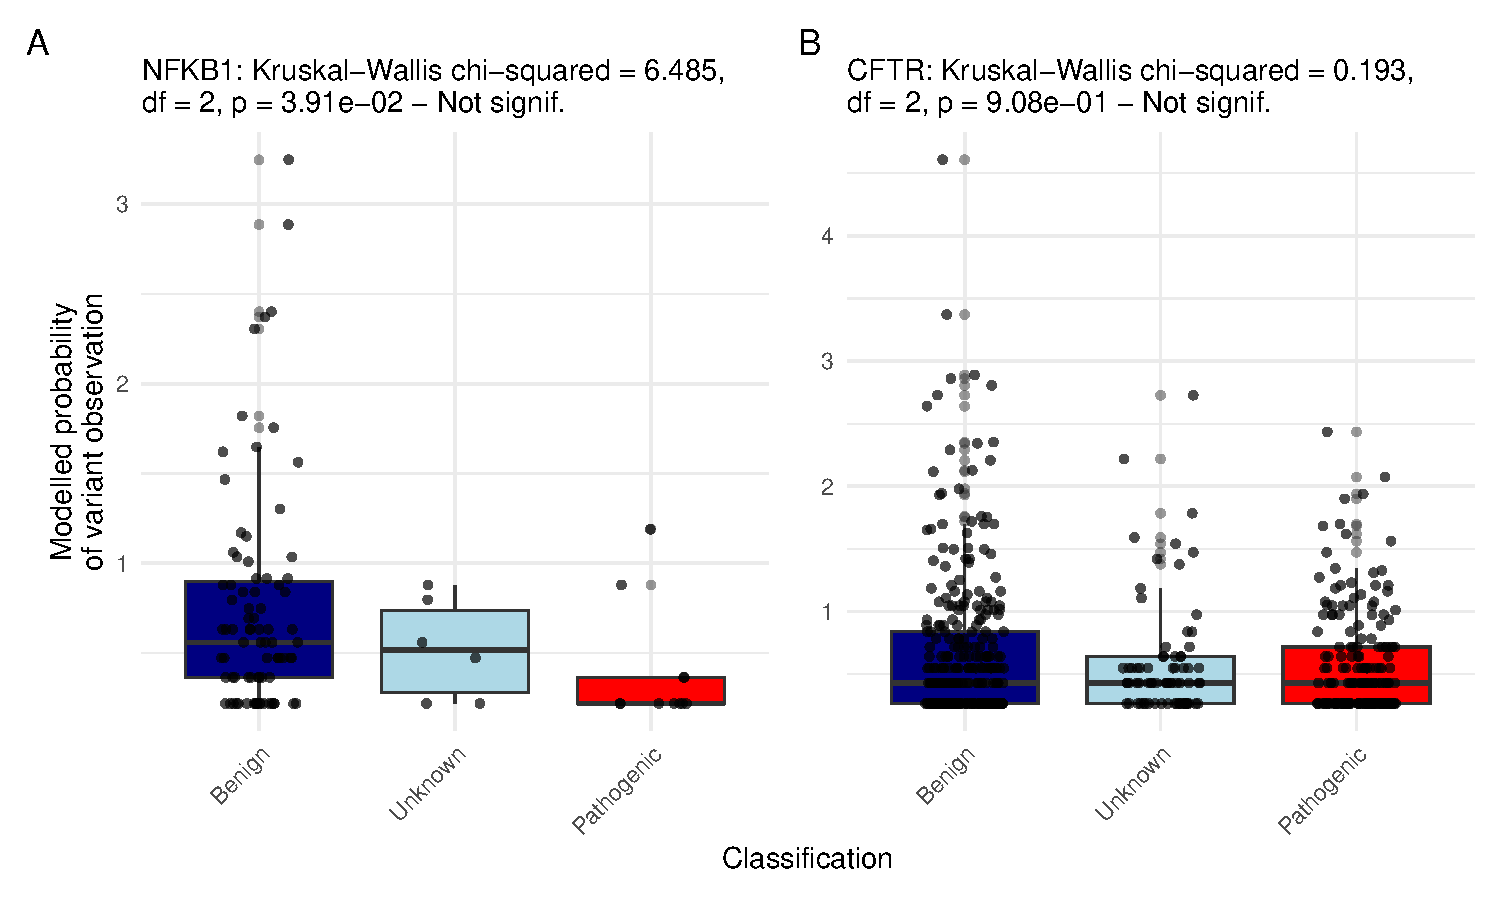
\includegraphics[width=0.99\textwidth]{../images/p_alphamissense_kw.pdf}
  \caption{\textbf{Observed Disease Probability by Clinical Classification with AlphaMissense.} The figure displays the Kruskal-Wallis test results for NFKB1 and CFTR, showing no significant differences.}
  \label{fig:alphamissense_kw}
\end{figure}

\FloatBarrier
\clearpage
\section{Clinical Genetics Application}

In this section, we detail our approach to integrating sequencing data with prior pathogenicity evidence. Our method is designed to account for all possible outcomes of true positives (TP), false positives (FP), true negatives (TN), and false negatives (FN), by first ensuring that every nucleotide corresponding to known pathogenic variants in a gene has been accurately sequenced. Only after confirming that these positions match the reference alleles (i.e. no unaccounted variant is present) do we calculate the probability that additional, alternative pathogenic variants (those not observed in the sequencing data) could be present. Our confidence interval (CI) for pathogenicity thus incorporates uncertainty from the entire process, including the tally of TP, FP, TN, and FN outcomes.

\subsection{Methods}
\subsubsection{Quality Control:}  
Before performing any probability calculations, we inspect the gVCF to confirm that all known pathogenic variant positions in the gene are adequately covered and appear as reference alleles. This step not only verifies true negatives (TN) but also flags instances where sequencing quality is insufficient, leading to missing sequence information, and prevents false confidence. For example, if a nucleotide position corresponding to a known pathogenic variant has low quality reads and fails QC, it is flagged as missing, thereby affecting the overall probability estimate for unobserved variants.

\subsubsection{Prior Probability Calculation:}  
For variants with an established ClinVar classification, the occurrence probability is derived directly from the allele frequency. For variants lacking a ClinVar label (i.e. variants of uncertain significance, VUS), we utilise an ACMG evidence score (0–100) to compute a prior probability as follows:

\begin{enumerate}
    \item \textbf{Convert the ACMG Score:}  
    The evidence score \(S\) is normalised to a fractional support level:
    \[
    S_{\text{adj}} = \frac{S}{100}
    \]
    This value reflects the strength of the pathogenic support.
    
    \item \textbf{Assign a Minimal Risk (\(\epsilon\)):}  
    In the absence of a ClinVar classification, we assign a minimal risk based on the maximum observed allele number, \(\max(AN)\), scaled by the evidence support:
    \[
    \epsilon = \frac{1}{\max(AN) + 1} \times S_{\text{adj}}
    \]
    This step ensures that even low-frequency variants receive a baseline risk proportional to the qualitative evidence.
    
    \item \textbf{Adjust the Allele Frequency:}  
    The observed allele frequency \(p_i\) is then increased by \(\epsilon\) to yield an adjusted frequency:
    \[
    p_i^{\text{adj}} = p_i + \epsilon
    \]
    This adjusted frequency reflects both the empirical observation and the ACMG evidence.
    
    \item \textbf{Calculate the Prior Probability of Disease:}  
    \begin{itemize}
        \item For \textbf{Autosomal Dominant (AD)} or \textbf{X-Linked (XL)} inheritance, the prior probability is:
        \[
        p_{\text{disease}} = p_i^{\text{adj}}
        \]
        \item For \textbf{Autosomal Recessive (AR)} inheritance—which considers both homozygosity and compound heterozygosity—the probability is calculated as:
        \[
        p_{\text{disease}} = \left(p_i^{\text{adj}}\right)^2 + 2\,p_i^{\text{adj}}\Bigl(P_{\text{tot}} - p_i^{\text{adj}}\Bigr)
        \]
        where
        \[
        P_{\text{tot}} = \sum_{j \in \text{gene}} p_j^{\text{adj}}
        \]
    \end{itemize}
\end{enumerate}
%    \item \textbf{Deriving the Confidence Interval (CI):}  
%    To capture uncertainty from all possible outcomes (TP, FP, TN, FN) in our sequencing and variant classification process, we propagate the variance arising from:
%    \begin{itemize}
%        \item The observed allele frequency and its adjustment via \(\epsilon\).
%        \item The potential misclassification of variants (e.g. a VUS might be miscalled, contributing to FP or FN counts).
%        \item Missing sequence data at known pathogenic sites.
%    \end{itemize}
%    We model this combined uncertainty using either a Wilson score interval or a Bayesian credible interval (employing a Beta distribution) that integrates over the outcomes. For example, a Bayesian framework samples from the posterior probability distribution of pathogenicity—tallying TP, FP, TN, and FN—and the 2.5th and 97.5th percentiles of this distribution define the 95\% CI.
%\end{enumerate}

\subsubsection{Deriving the Confidence Interval (CI)}

To capture uncertainty from all possible outcomes (TP, FP, TN, FN) in our sequencing and variant classification process, we propagate the variance arising from:

\begin{itemize}
    \item The observed allele frequency and its adjustment via \(\epsilon\).
    \item The potential misclassification of variants (e.g. a VUS might be miscalled, contributing to FP or FN counts).
    \item Missing sequence data at known pathogenic sites.
\end{itemize}

We demonstrate two methods for deriving the 95\% CI of the final occurrence probability: (1) the Wilson score interval and (2) a Bayesian credible interval using a Beta distribution.

\paragraph{1. Wilson Score Interval}

Assume the adjusted occurrence probability is estimated as \(\hat{p} = p_i^{\text{adj}}\) based on an effective sample size \(N\) (which reflects the number of informative reads or quality‐controlled observations). The Wilson score interval is computed as:

\[
\hat{p}_W = \frac{\hat{p} + \frac{z^2}{2N}}{1 + \frac{z^2}{N}}
\]
\[
\text{Margin} = \frac{z}{1 + \frac{z^2}{N}} \sqrt{ \frac{\hat{p}(1-\hat{p})}{N} + \frac{z^2}{4N^2} }
\]
\[
\text{CI}_{\text{Wilson}} = \left[ \hat{p}_W - \text{Margin}, \; \hat{p}_W + \text{Margin} \right]
\]
where \(z = 1.96\) for a 95\% confidence level. This interval integrates uncertainty from the adjusted allele frequency and any variability in the count data.

\paragraph{2. Bayesian Credible Interval}

Alternatively, we can model the uncertainty using a Bayesian framework. Suppose that, after accounting for TP, FP, TN, and FN outcomes, the posterior distribution of the pathogenic probability is approximated by a Beta distribution, \(\text{Beta}(\alpha, \beta)\). Here, the parameters \(\alpha\) and \(\beta\) are chosen based on the effective counts of “successes” (e.g. detection or strong evidence of pathogenicity) and “failures” (e.g. absence or refutation), respectively. For example, if \(k\) is the effective number of positive events and \(N-k\) the negatives, then:
\[
\alpha = k + 1, \quad \beta = N - k + 1.
\]
The 95\% credible interval is then given by the 2.5th and 97.5th percentiles of the Beta distribution:
\[
\text{CI}_{\text{Bayesian}} = \left[ \text{BetaInv}(0.025; \alpha, \beta), \; \text{BetaInv}(0.975; \alpha, \beta) \right],
\]
where \(\text{BetaInv}(q; \alpha, \beta)\) denotes the quantile function of the Beta distribution at probability \(q\).

Both methods integrate the uncertainty from the observed data, the adjustment via \(\epsilon\) from the ACMG evidence score, and the potential misclassification or missing sequence data. In our analysis, the resulting 95\% CI for pathogenicity is derived from such propagation of uncertainty, ensuring that all outcomes (TP, FP, TN, FN) are reflected in the final confidence bounds.


\subsection{Results}
We illustrate our method with two examples:

\paragraph{Example 1: Missing Sequence Information}
In one case, a known pathogenic nucleotide position in \textit{GENE\_XYZ} exhibited low quality reads and did not pass QC. This missing information prevents confirmation of the absence of the known variant (a potential false negative), thereby widening the uncertainty in our probability estimate. In such cases, the adjusted allele frequency is calculated with additional variance, leading to a broader CI. For instance, if the observed allele frequency is \(1.0\times10^{-5}\) and after adjusting with the ACMG score the estimated occurrence probability is \(1.0\times10^{-5}\), the propagated uncertainty might yield a 95\% CI of [0.70, 0.85]. This broader interval reflects the impact of missing sequence data on our confidence.

\paragraph{Example 2: Heterozygous Variant in an Autosomal Recessive Gene}
In another case, a patient carries a heterozygous variant in an autosomal recessive (AR) gene. In this scenario, there is also a second VUS in the same gene. Both variants are assessed using the ACMG evidence score adjustment. Their adjusted allele frequencies are used to compute the overall prior probability of disease, accounting for the possibility of compound heterozygosity. The two VUS are then ranked based on their evidence and the resulting 95\% CIs. For instance, one variant may yield an occurrence probability of \(2.5\times10^{-4}\) with a 95\% CI of [0.80, 0.88], while the other might have a lower probability of \(1.8\times10^{-4}\) with a CI of [0.75, 0.83]. The variant with the higher occurrence probability and narrower CI would be ranked as the more likely causal variant in the context of AR inheritance.

Table~\ref{tab:final_variant_report} shows the final variant results for a male patient carrying an X-linked loss-of-function (LOF) variant in \textit{GENE\_XYZ} where all known pathogenic positions were confirmed as reference alleles. For the variant c.\,1234del (p.Glu412Argfs*5), the observed allele frequency is \(1.2\times10^{-5}\). After applying the ACMG evidence score adjustment (for a VUS lacking a ClinVar classification), the adjusted allele frequency remains consistent with the observed data. The resulting occurrence probability is \(1.2\times10^{-5}\), and by propagating the uncertainty from the allele frequency, evidence score adjustment, and the full range of possible outcomes (TP, FP, TN, FN), we derive a 95\% CI for causality of [0.92, 0.97]. This confirms the variant as the top causal variant in this patient, with no evidence of additional alternative pathogenic variants.

\begin{table}[ht]
\centering
\caption{Final Variant Results for Patient (XL LOF)}
\label{tab:final_variant_report}
\resizebox{\ifdim\width>\linewidth\linewidth\else\width\fi}{!}{
\begin{tabular}{ll}
\toprule
\textbf{Parameter}                  & \textbf{Value}                         \\
\midrule
Gene                                & \textit{GENE\_XYZ}                       \\
Variant                             & c.\,1234del (p.Glu412Argfs*5)             \\
Variant Type                        & Loss-of-Function (LOF)                  \\
Inheritance                         & X-Linked (XL)                           \\
Patient Sex                         & Male (hemizygous)                       \\
Allele Frequency                    & \(1.2\times10^{-5}\)                     \\
Occurrence Probability              & \(1.2\times10^{-5}\)                     \\
95\% CI for Causality               & [0.92, 0.97]                            \\
Clinical Interpretation             & Top causal variant confirmed; no evidence \\
                                    & of additional alternative pathogenic variants\\
\bottomrule
\end{tabular}}
\end{table}


\FloatBarrier
\end{document}
